\chapter{\texorpdfstring{Potassium (\ce{K+}) channels}{Potassium channels (K+
channels)}}
\label{chap:potassium-channels}

\def\SK{{\text{SK}}}
\def\KACh{{\text{{KACh}}}}
\def\TEA{{\text{TEA}}}
\def\Erev{{\text{E}_{\text{rev}}}}
\def\KtwoP{{\text{K}_{\text{2P}}}}

Julius Bernstein (1839-1917) is a German physiologist who first explained the
origin of ``resting potential'' and ``action potential'' of nerves and muscles
\footnote{\url{http://www.st-andrews.ac.uk/~wjh/neurotut/mempot.html}}.
In 1902, he developed the first quantitatively model of membrane theory. Along
with this model, he also (in 1902, 1912) first pointed out the existence of
transmembrane proteins in excitable cell membranes serving as ion channels that
are selective to $\K$ ions (review: \citep{seyfarth2006}). At that time, the $\K$
channels were found to be \textcolor{red}{outward rectifying potassium
conductance} (Sect.\ref{sec:rectification}), i.e.
Sect.\ref{sec:K_outward-rectifier}.
  
In 1949, Sir Bernard Katz described a novel potassium channel with conductance
that are \textcolor{red}{inward rectification}~\citep{Katz1949}. As it's different with
what every one think $\K$ current should be, this channel was first given the
name {\it anomalous rectifier} (Sect.\ref{sec:Kir_family}).

\begin{figure}[hbt]
  \centerline{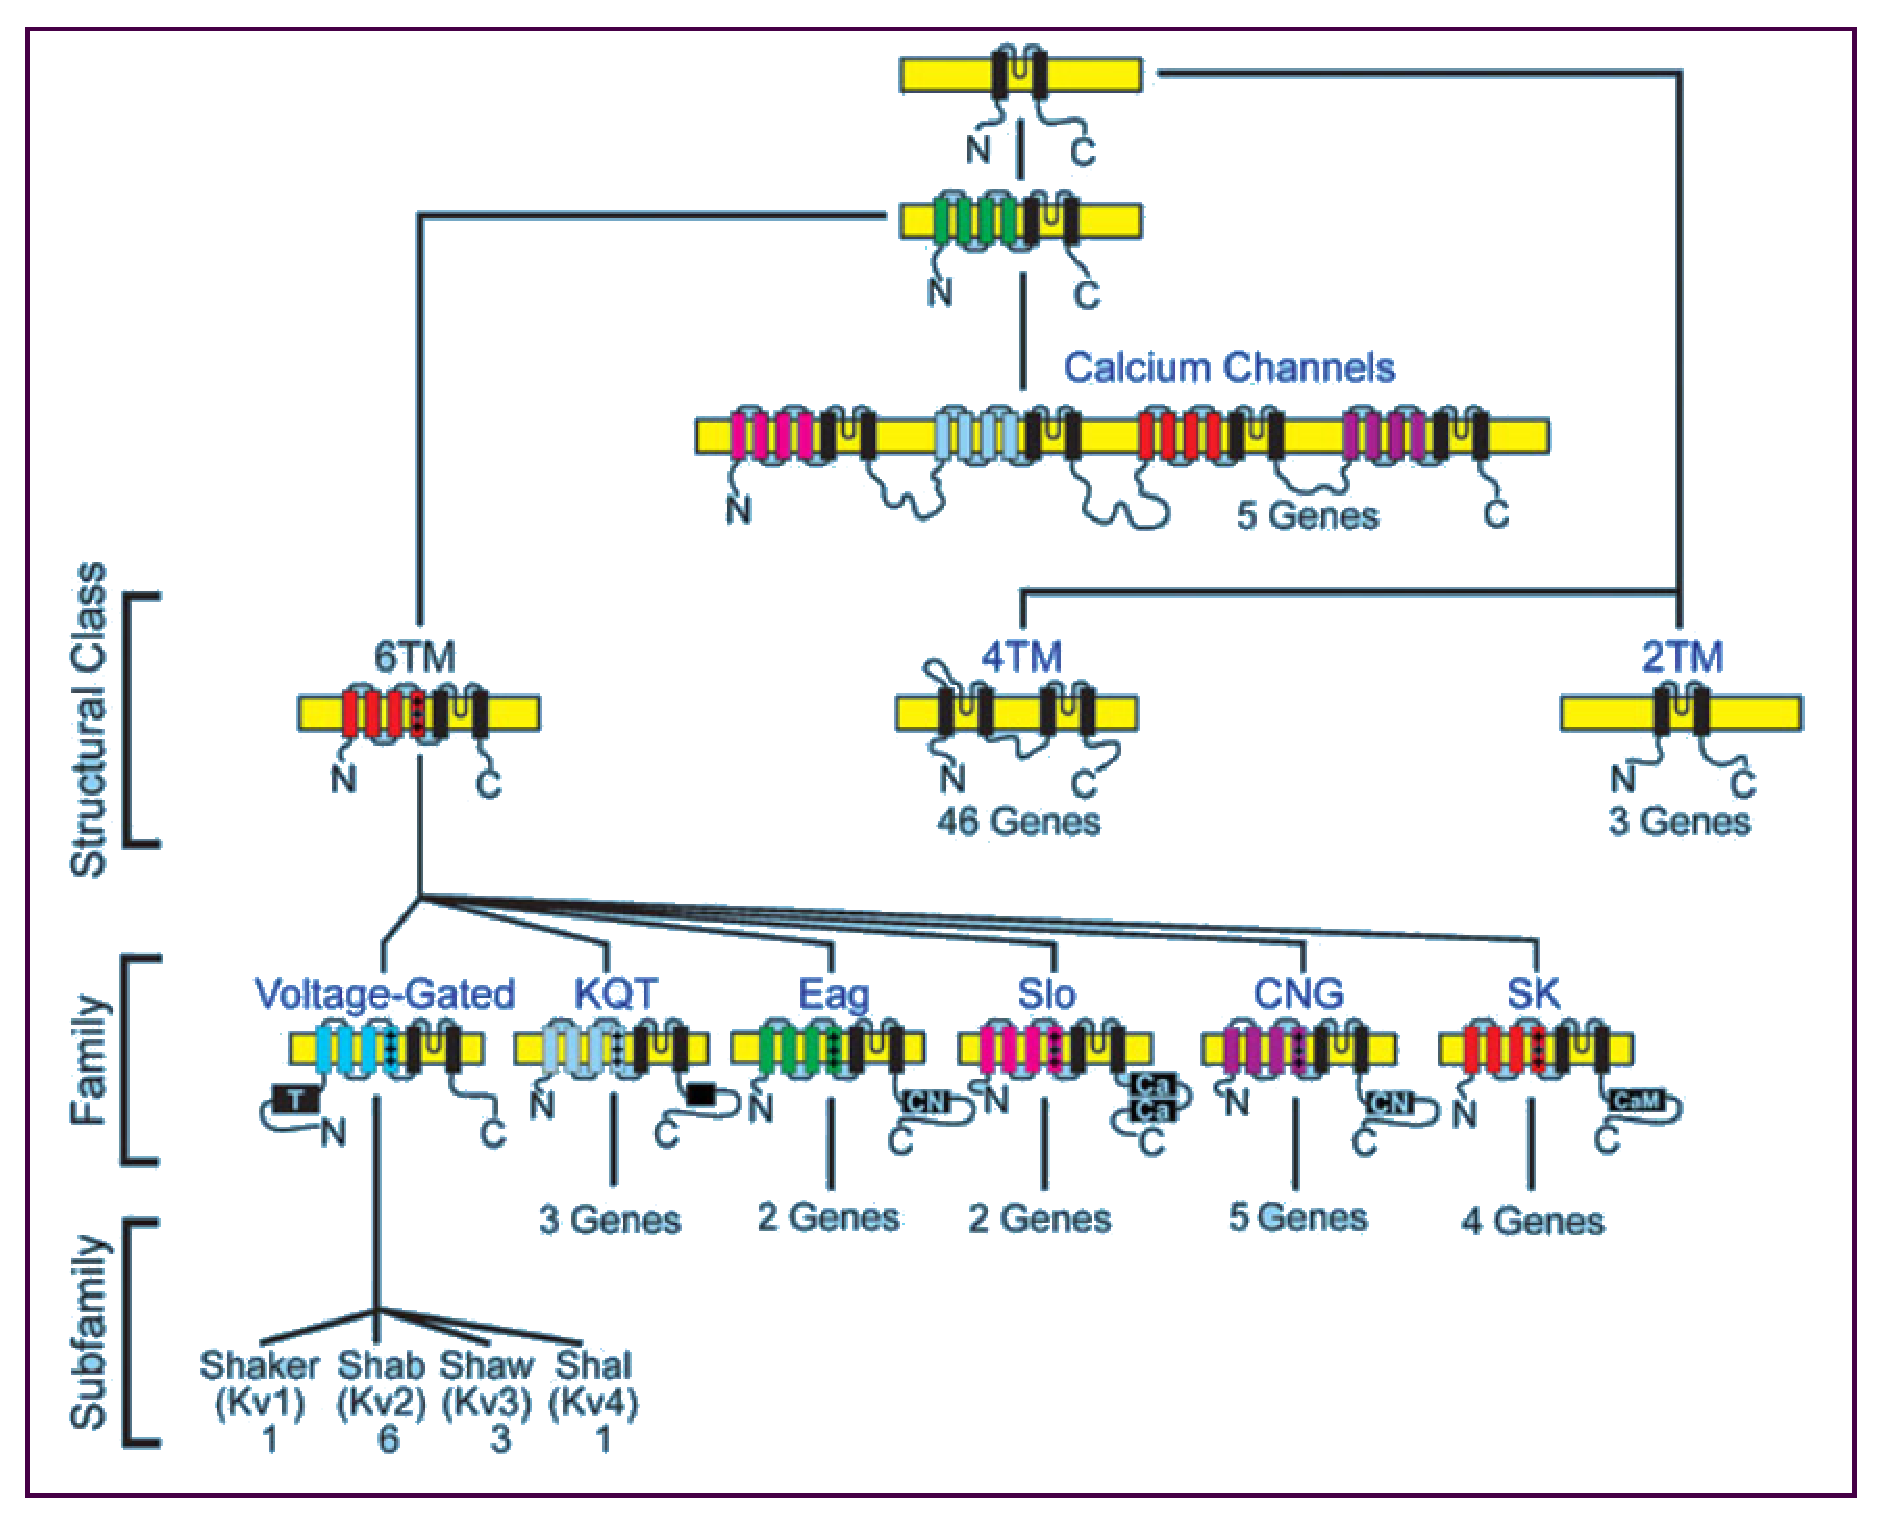
\includegraphics[height=7cm,
    angle=0]{./images/K-channel_classification.eps}}
\caption{3 structural classes (6TM/P, 4TM/P and 2TM/P). In {\it C. elegans},
6TM/P structural class is subdivided into 6 families; and only
voltage-gated family is subdivided into subfamilies \citep{wei1996}}
\label{fig:K-channel_classification}
\end{figure}

Since then, there are many other types of $\K$ current have been discovered.
Some $\K$ channels open rapidly, and some, slowly; some
voltage-dependent, and some calcium-dependent; some have large conductance, some
with small conductance; some transport $\K$ more easily inward, some more easily
outward (upon transmembrane potential depolarization).
As such, K+ channels are the largest and most diverse type of ion channel
found in nature. $\K$ channels are the founding members of the S4-superfamily of ion
channels. We'll discuss $\K$ channels's models in Chap.\ref{chap:K_model}.

\section{Introduction}
\label{sec:introduction-4} 

The completion of the sequencing of the genomes of {\it Drosophila melanogaster}
(fruit fly) and {\it Anopheles gambiae}, which belong to the same order - the
Diptera - allows us to compare and contrast K+-channel genes and gene families
present within the genomes of two Dipterans.

There are about 30-100 $\K$ channel genes in each organism (humans, Drosophila,
Caenorhabditis elegans) ~\citep{Miller2000}.
The size and diversity of potassium channels were not fully understood until the
complete genome sequencing of {\it C. elegans} in 1998 with about 70 genes
encoding potassium channels. Luckily, all types of potassium channels found in
C. elegans are conserved in mammals, which made it easier to infer the
functional role of potassium channels in mammals.
So, {\it C. elegans}, even though a simple species with only 302 neurons, has
been a widely used for studying K+ channels.

\begin{mdframed}
  Ion channels, as special transmembrane proteins, are believed to
  undergo a series of conformational change that allow the opening
  (gating) and closing (inactivation) swiftly. 
  
  Given that the volume of a neuron about $10^{-12}$ ml, the intracellular
  \ce{K+} concentration is 100 mM (about $10^8$ ions), the rate of permeability
  of \ce{K+} is $10^7$ per second (near diffusion-limited rate); then with 10
  channels opening, it could drain all \ce{K+} ions in about 1 seconds. Thus,
  the opening and closing of \ce{K+} need to be brief and fast (in millisecond)
  \citep{choe2002pcs}.
\end{mdframed}


\subsection{Structure of a subunit}
\label{sec:structure-K-channel}

A protypical potassium channel is a tetrameric protein formed by 4 identical
subunits (Review: ~\citep{choe2002pcs}).
A canonical structure of a subunit is 2TM/P: 2 inner helices and a P loop
between them.

There are different types of subunits, and they form different
subfamilies of $\K$ channels (Sect.\ref{sec:K_channel-nomenclature}).
There are two major high-level structure for a subunit:
\begin{itemize}
  \item 2TM/P - Sect.\ref{sec:2TM/P}
  \item 6TM/P - Sect.\ref{sec:6TM/P}
\end{itemize}
However, there are other types of \ce{K+} channels that may differ in some
parts, as shown in Fig.~\ref{fig:K_channel2}. 

\begin{figure}[hbt]
  \centerline{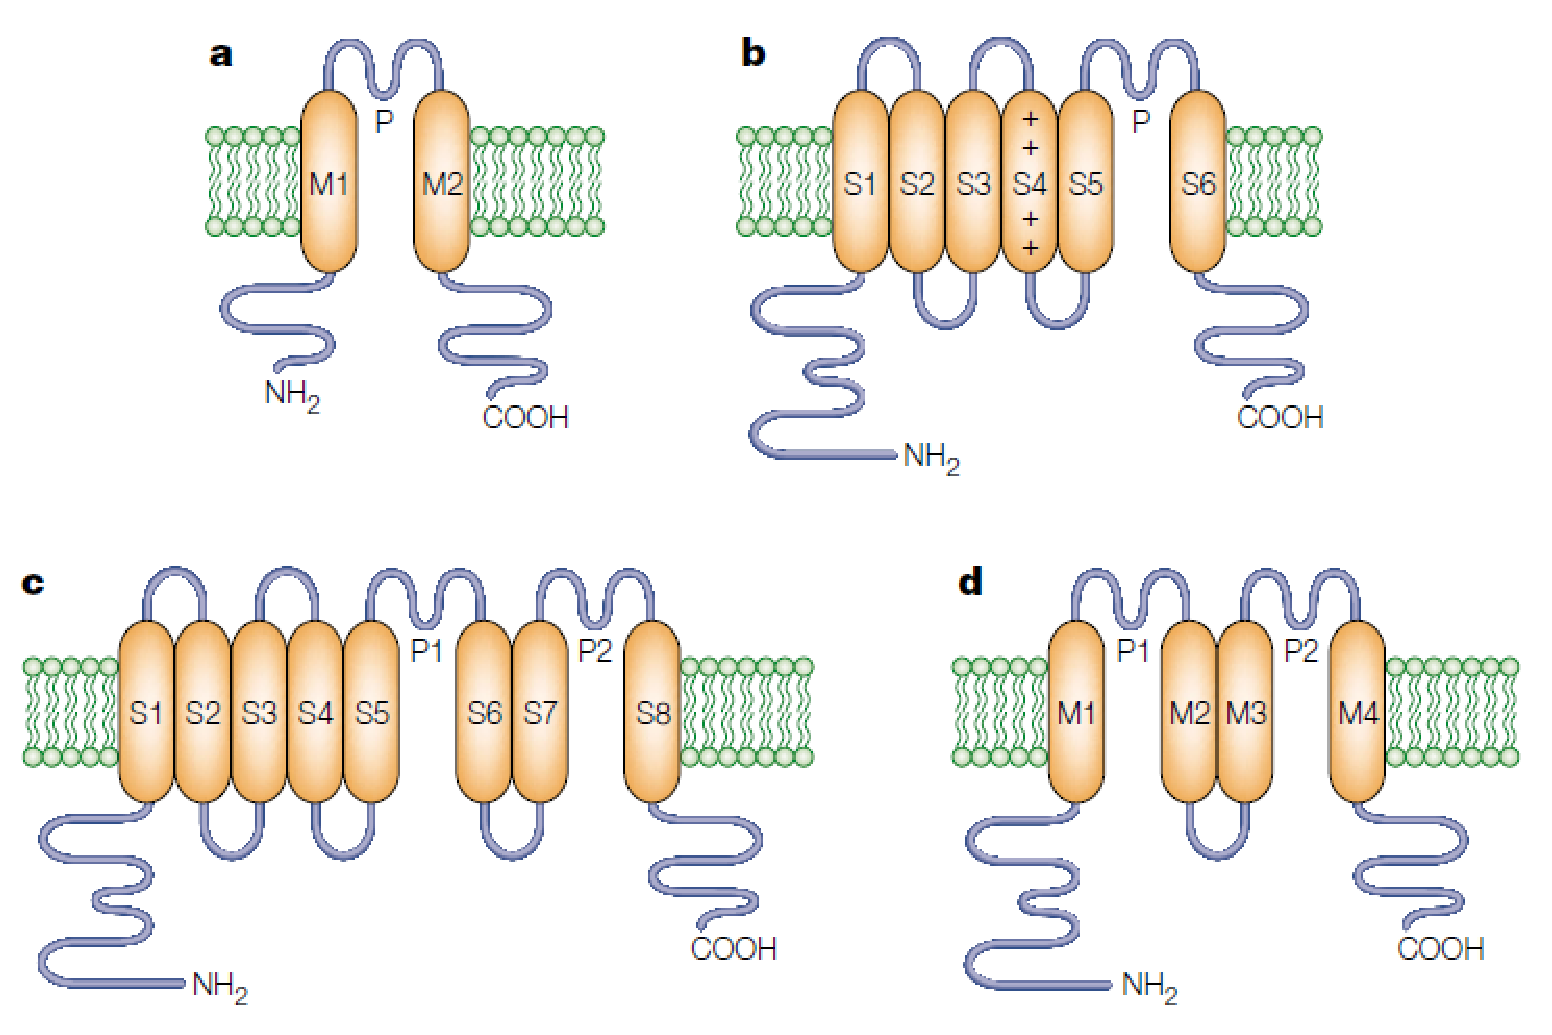
\includegraphics[height=5cm,
    angle=0]{./images/K_channels2.eps}}
\caption{4 main classes of a subunit in \ce{K+} channels: (A) 2TM/P, (B) 6TM/P
(4 transmembrane helices (S1-S4) precede 2TM/P), (C)
 8TM/2P (hybrid of 2TM/P and 6TM/P), (D) 4TM/2P}
\label{fig:K_channel2}
\end{figure}

The S5-S6 (in the case of 6TM/P) or M1-M2 (in the case of 2TM/P) is known as the
ion-permeation module. Between them, the  short stretch of about 20 amino acids
known as the P (i.e. pore forming) region which is highly conserved: it is this
region which gives K+ channels their remarkable ability to discriminate between
K+ and other cations with almost perfect distinction, yet facilitate the
transmembrane passage of more than a million ions per second. The conserved
sequence is {\bf T-X-G-X-G} and is known as the 'K+ channel signature sequence'.

The structure of each subunit is discussed below. The different types of
potassium channel family will be discussed in
Sect.\ref{sec:K_channel-nomenclature}.

\subsection{-- 2TM/P}
\label{sec:2TM/P}

\textcolor{red}{\bf 2TM/P}: The subunits of (evolutionary) oldest potassium
channels consist of  2 transmembrane (TM) helices, and one intervening pore-loop
(P loop).  The 2TM/P subunit of KcsA (Sect.\ref{sec:KcsA}) has only 2
transmembrane segments (outer-$\alpha$ helix M1 and inner-$\alpha$ helix M2
linked by reentrant loop P) with a central pore.  The pore-forming 2TM/P domain
is flanked by cytoplasmic, protein-interacting domains
\begin{enumerate}
  \item  The amino-terminal tetramerization domain that is a conserved among
  voltage-gated $\K$ channels
  
  \item A carboxy-terminal, protein-interacting domain that is characteristic of
  inwardly-rectifying $\K$ channels.
  
  \item A carboxy-terminal, nucleotide-binding domain known as {\bf KTN
  NAD-binding domain} that is highly conserved across all prokaryotic
  $\K$-transport systems, and in plants.
  
  This is related to {\bf RCK domain} (which regulate the conductance of $\K$
  ions) in eukaryotic BK $\K$ channel - Sect.\ref{sec:BK-current}.
\end{enumerate}

$\K$ channels with 2TM/P per subunit:
\begin{enumerate}
  \item KcsA - Sect.\ref{sec:KcsA}

 
  \item Kir - Sect.\ref{sec:Kir_family}, Fig.\ref{fig:K_channel}(B).
  
\end{enumerate}

The $\K$ selectivity is associated with this the motif {\bf TVGYG}
(Thr-Val-Gly-Tyr-Gly) ({\it selectivity filter}) located in a re-entrant loop
P. There are 4 copies of the motif forming the pore, and in the case of KCsA;
(using resolution 3.2$\AA$) the narrowest part of the channel filter is
about 2.7 $\AA$ in diameter, and about 12$\AA$ long.

The crystal structure of KcsA shows the channel filter is $\approx 12\AA$ long
and $\approx2.5\AA$ in diameter. The highly selectivity of $\K$ channels is
achieved by a number of 'stereochemical' checkpoints. Each checkpoint has 4
oxygen atoms, and is repeated 5 times every $\approx 3\AA$ along the filter
(Review: \citep{choe2002pcs}). At 2.0$\AA$ resolution of KcsA, six K+-binding
sites have been accurately visualized along the selectivity filter - four
internal (P1-P4) and two external (P0 and P5).

\begin{figure}[hbt]
  \centerline{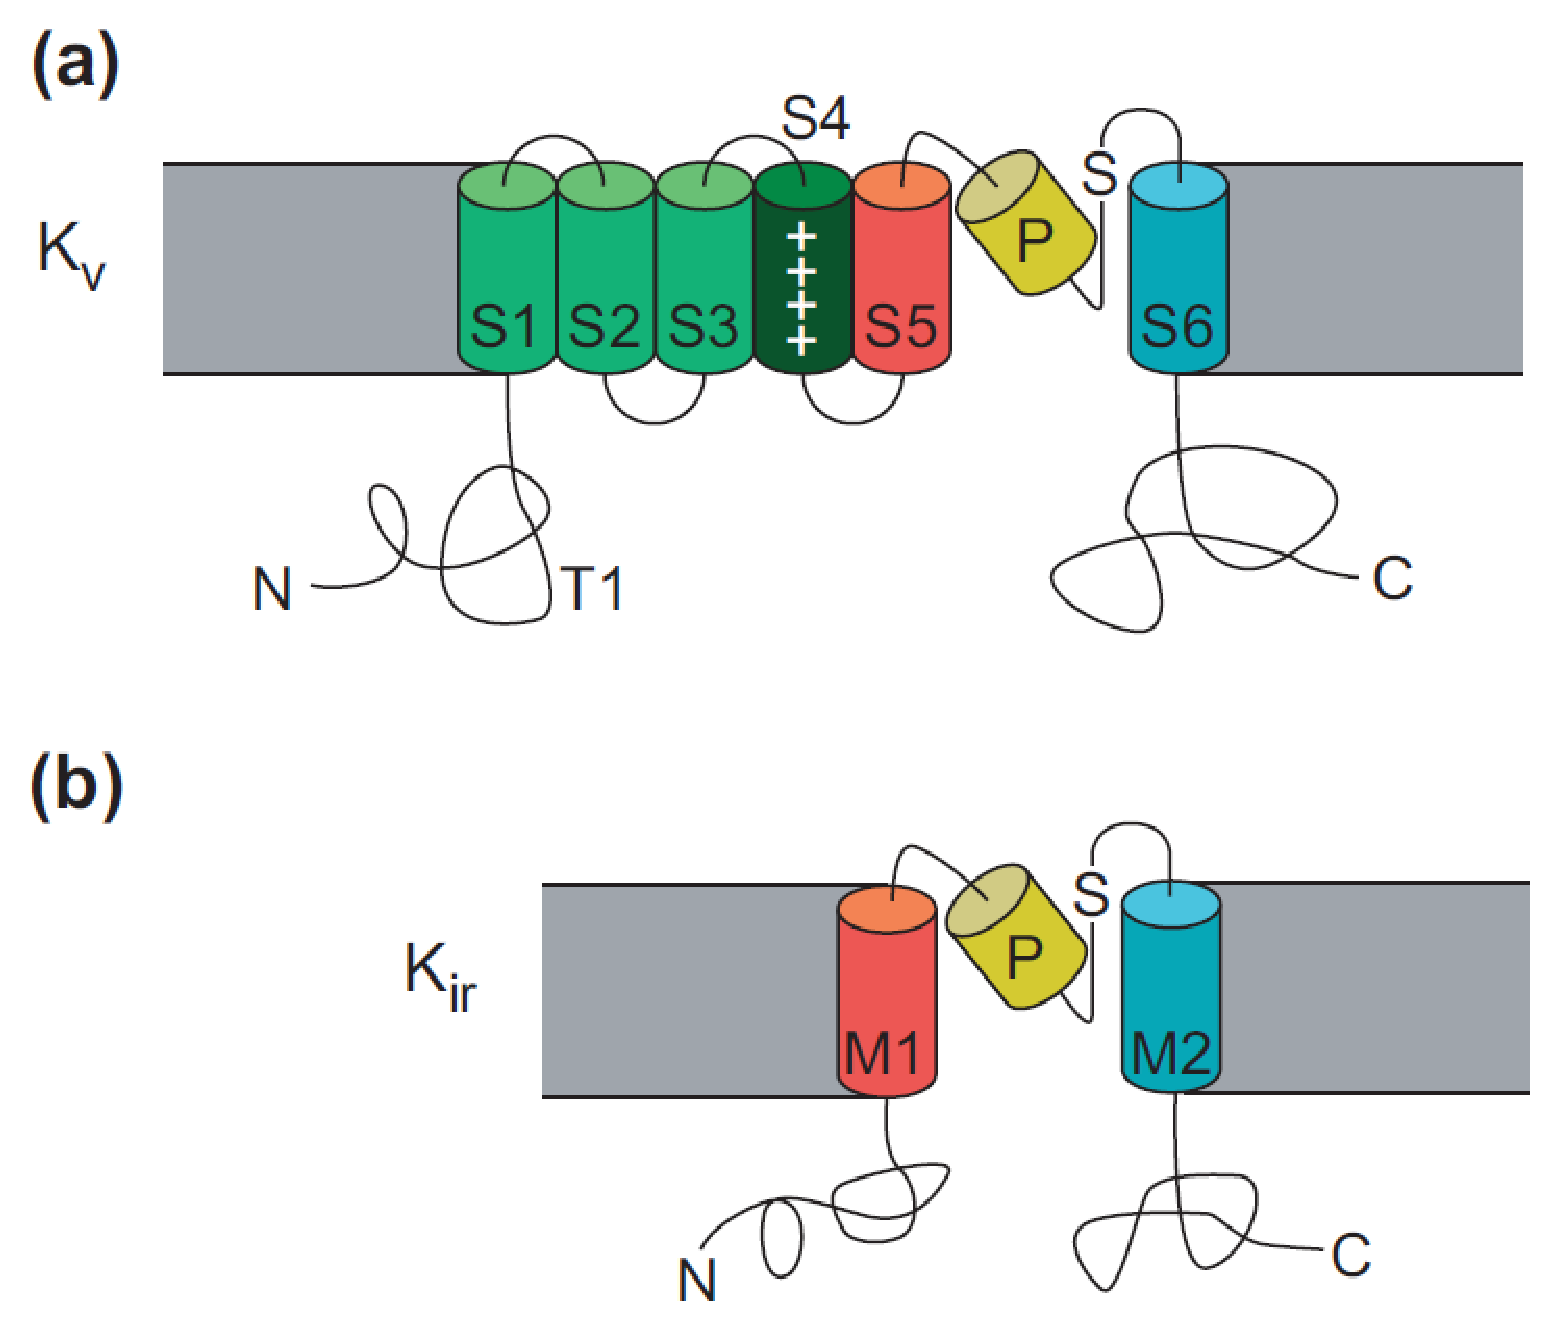
\includegraphics[height=5cm,
    angle=0]{./images/K_channels.eps}}
  \caption{(a) 6TM/P found in Kv-family potassium channels; (b) 2TM/P found in
  Kir potassium channel. {\bf NOTE}:
  Transmembrane helices are numbered S1-S6 in $\Kv$; M1 and M2 in $\Kir$ with S4
  is voltage-sensing domain; P is pore helix; S is signature sequence
  (TMxTVGYG); N is amino terminus; C is carboxyl terminus; T1 is conserved T1
  domain \citep{Miller2000}. The T1 domain is attached to the rest of the
  channel by four tethers that define four lateral openings through which K+
  ions enter the channels' pores.
pore.}
\label{fig:K_channel}
\end{figure}


\subsection{-- 4TM/P}
\label{sec:4TM/P}

\textcolor{red}{\bf 4TM/P}:

In {\it C. elegans}, surprisingly, the most frequently encountered type of
potassium channel belongs to the 4TM/P class of channel with 46 known genes.
The K+ channels has 4 subunits: each is a 4TM/P with 4 transmembrane $\alpha$
domain and Pore-loop. The $\alpha$ is the non-inactivating Kv component.

In Drosophila there are approximately 11 genes encoding channels of this
type (Adams et al., 2000; Littleton and Ganetzky, 2000; and Rubin et al., 2000),
while in humans there are approximately 15 genes.


\subsection{-- 4TM/2P}
\label{sec:4TM/2P}

Similar to 8TM/2P (Sect.\ref{sec:8TM/2P}), {\bf 4TM/2P} subunit has two 2TM/P
motifs (Sect.\ref{sec:2TM/P}).

Example:
\begin{itemize}
  \item leak $\K$ current - Sect.\ref{sec:leak-K+-current}
\end{itemize}


\subsection{-- 6TM/P}
\label{sec:6TM/P}

\textcolor{red}{\bf 6TM/P}: $\K$ channels in vertebrate have 6 TM segments per
subunit plus N-terminal domain and ancillary subunits. The four transmembrane
(4TM) helices (S1-S4) precede the 2TM/P in voltage-gated K+ channels to endow
the channel with the capability to sense and respond to the change in membrane
potential. As you see later, the presence of S4 motif is critical for
voltage-sensitive.

The 6TM/P are the predominant class of among ligand-gated voltage-gated \ce{K+}
channels.
\begin{itemize}
  \item The core-forming domain S5-P-S6 is homologous to M1-P-M2 in KcsA
  (yet with 30\% sequence similarity).

The S5-P-S6 section resembles the 2TM-1P subunit; yet it is the S4 segment that 
provides voltage-dependent behavior.

  \item  6 \ce{K+}-binding sites: 4 internal (P1-P4) and 2 external (P0, P5).  

  \item S4 is voltage-sensing domain: The gating (opening) is triggered by the
voltage depolarization, along with the conformational change in S4 membrane
helix. \textcolor{red}{S4 is thus suggested as a voltage sensor}. 

The four transmembrane helices S1-S4 form the voltage-sensing module and
response of voltage change in transmembrane potential. 

  \item $\K$ channels with two P-domains are usually highly regulated $\K$
  selective leak channels (Sect.\ref{sec:leak-K+-current}).

  \item Different ancillary subunits - Sect.\ref{sec:Kv-ancillary-subunits}
  
%  \item 
\end{itemize}

\subsection{-- 8TM/2P}
\label{sec:8TM/2P}

Similar to 4TM/2P (Sect.\ref{sec:4TM/2P}), {\bf 8TM/2P} subunit has two 2TM/P
motifs (Sect.\ref{sec:2TM/P}). 8TM/2P so far has only been found in yeast.

Example:
\begin{itemize}
  \item TOK-1 - Sect.\ref{sec:TOK-1_current}
\end{itemize}


\subsection{Regulatory factors}
\label{sec:K_regulatory-factors}

As mentioned above, a prototypical \ce{K+} channel has some $\alpha$-helix
subunits with one or two short {\bf P loop}, Fig.\ref{fig:K_channel2}\footnote{P
loop - a short amino acid sequence that dips into the membrane without fully
crossing it.
Primary P loop in K channel has the sequence Thr-Val-Gly-Tyr-Gly}. P-loop
contains the sequence T/SxxTxGxG, which is the $\K$ selectivity sequence.
The carboxyl-terminal, protein-interaction domain is the characteristics for the
{\it inwardly rectifying $\K$ channels}. Another part, the carboxyl-terminal,
nucleotide-binding domain (known as {\it KTN NAD-binding domain} - PFAM number
PF02254) is highly conserved across all prokaryotic \ce{K+}-transport system and
serves as the universal regulator in determining the $\K$ conductance.

\begin{enumerate}
\item $\Kv$ are activated by $V_m$ depolarization

\item $\Ca$-activated $\K$ channels responds to $[\Ca]_i$. Some are sensitive to
both $V_m$ and cytosolic $[\Ca]_i$.

\item $\Kir$ are gated by different intracellular signals,
  e.g. G-protein, nucleotides, or polyamines (spermine, spermidine and
  putrescine).
\end{enumerate}

In addition to the intrinsic mechanism that regulates the gating,
protein-protein interaction can also affect the channel function. The best known
case is the inwardly rectifying \ce{K+} channel Kir3 (Sect.\ref{sec:Kir3.x}) by
{\bf G-protein-coupled receptors} (G$\beta\gamma$ complex).
The most striking example is the interaction between the amino-terminal domain
of Kv4 channels and the protein KchiP ($\Kv$ channel in the human encoded by
KCNIP1 gene) which enhances inactivation and recovery rates~\citep{choe2002pcs}.
In addition to the above factors, protein phosphorylation is often found to
modulate the sensitivity of $\K$ channels.

\subsection{Potassium concentration}
\label{sec:concentration-K+-ion}

[K]i = 140 mM, and [K]o = 3 mM.

\subsection{K+ channel inactivation}
\label{sec:K+-channel-inactivation-mechanism}


SUMMARY: The inactivation can occur either at the cytoplasmic side (N-type
inactivation) or extracellular side (C-type inactivation),
Fig.\ref{fig:Kchannel_inactivation}.

In the late 70s, Armstrong and Bezanilla in an effort to explain the mechanism
of A-type inactivation, proposed the 'ball-and-chain' model
(Sect.\ref{sec:ball-and-chain-model-of-inactivation}).
The self-inactivating property of the $\Kv$ channels (Sect.\ref{sec:Kv_channel})
was hypothesized as an inactivating ball connecting to the T1 domain
\citep{hoshi1990}.

\begin{figure}[hbt]
  \centerline{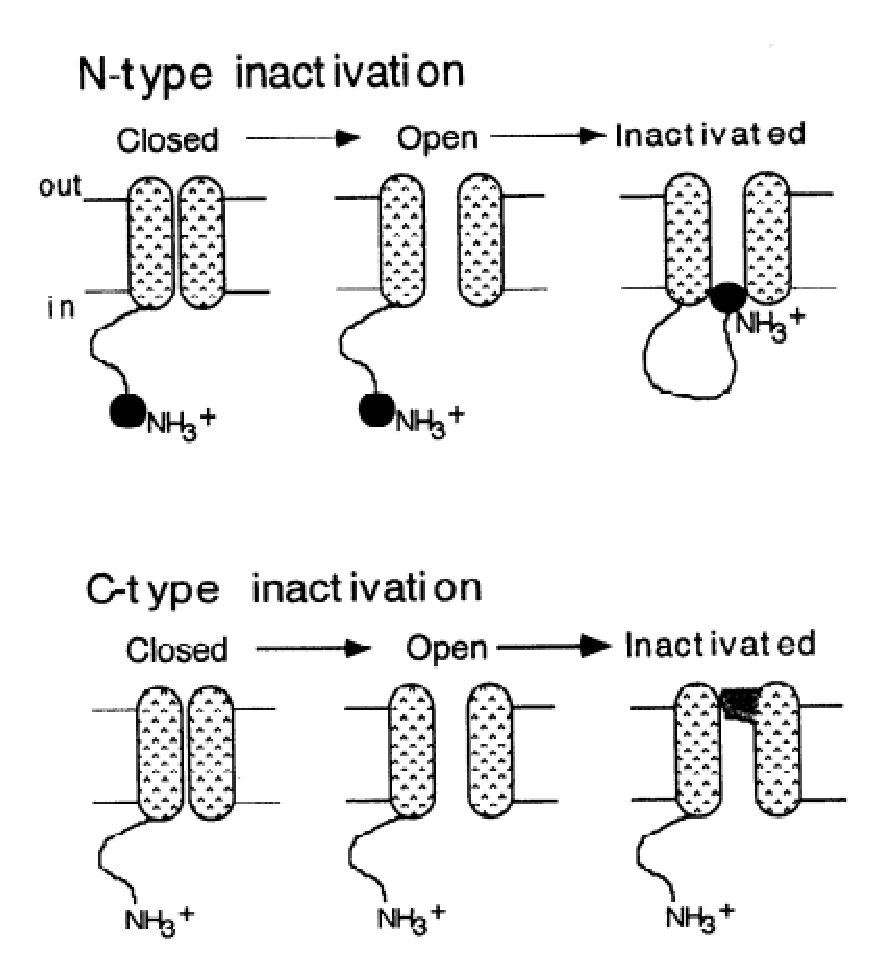
\includegraphics[height=5cm,
    angle=0]{./images/inactivation_mechanism.eps}}
  \caption{Mechanism of channel inactivations \citep{sanguinetti1997}}
  \label{fig:Kchannel_inactivation}
\end{figure}

Many $\K$ channels inactivate {\bf rapidly by N-type inactivation} and slowly by
C-type inactivation. However, $I_\Kr$ is different; it has C-type inactivation
much faster than transition from closed to open state.

\section{Ancillary subunits of K+ channels}
\label{sec:Kv-ancillary-subunits}

For review: \citep{sansom2002}

\begin{itemize}
  
  \item inactivation domain (ball) at N-terminus: block intracellular ion
  conduction pathway
  
  \item T1 domain (NTD) at N-terminus: to stabilize the functional
  tetrameric channel.

Subunits from the same families can assemble to form a heterotetrameric
channels. This does not happen with subunit from different families. The
polypeptide chain - known as T1 tetramerization domain - with 131 amino acids
that immediately precede S1 is to stabilize the functional tetrameric channel.
  
  \item Kv $\beta$ at separate chain: Sect.\ref{sec:beta-subunit-K+-channels}
  
  \item Calmodulin-binding domain (CaMBD) at (intracellular) C-terminus:
  $\Ca$-sensing domain, i.e. channel open when $\Ca$ bind to the EF-hand in
  N-lobe of CaM.
  
  \item RCK domain at (intracellular) C-terminus: $\Ca$-sensing domain, which 
   is found not only in eukaryotic BK channels, but also in
  many prokaryotic K channels and in prokaryotic transport
  system subunits such as TrkA
  
  \item \label{sec:minK-subunit} minK protein act as a $\beta$-subunit that
  coassembles with an $\alpha$-subunit, KvLQT1, to form $I_\Ks$ channel
  (Sect.\ref{sec:IKs_current}). minK ($K_\min$) is the smallest $\K$ channel
  protein known (with 130amino acids and a single transmembrane domain), and
  regulate the slow component of delayed rectifier current $K_s$.
 
 \item  KChIP subunit - Sect.\ref{sec:KChIP}
\end{itemize}

\subsection{Kv-beta subunit}
\label{sec:beta-subunit-K+-channels}

A-type channels contain $\beta$-subunits as regulatory proteins.
Post-translational modifications, e.g. protein phosphorylation, are also pivotal
in A-type K+ channel modulation as a temporary change to the function of K+
channels. These two fundamental modes of modulation can co-exist in the same
channel protein.

Kv$\beta$ subunits were first found in bovine rat extracts (Parcej et al.,
1992). They are soluble proteins lacking transmembrane domains, or
N-glycosylation consensus sites. The N-terminal of Kv$\beta$ subunits are
variable, i.e. in some isoforms the first 20 residues constitute the
inactivating ball ($\beta$-ball) that confer the A-type characteristics to
non-inactivating $\alpha$-subunits. 
% Parcej DN, Scott VE, Dolly JO. Oligomeric properties of alphadendrotoxin-
% sensitive potassium ion channels purified from bovine
% brain. Biochemistry 1992; 31: 11084-8.
Since then there are 3 highly related distinct $\beta$-subunits 
\begin{itemize}
  \item from rat brain: Kv$\beta$1, Kv$\beta$2
  
  \item from ferret: Kv$\beta$3
  
  \item from human heart: hKv$\beta$3
\end{itemize}

Four major classes of ancillary subunits of A-type channels have been described
which differ in their sequences, structures, effects and $\alpha$-subunit
specificity:

\begin{enumerate}
  \item Kv$\beta$2 subunit: a soluble protein with aldo-keto-reductase (AKR)
  activity. AKR is an enzyme that catalyzes a redox reaction using an NADPH
  cofactor. 
  
  Kv$\beta$2 has no inactivation ball therefore it does not convert their partners
  into A-type channels although it can accelerate inactivation kinetics..
  
  The structures of rat Kv$\beta$2 [34] alone and in complexes formed with the T1
  domain of rat Kv1.1; and entire rat Kv1.2 

  It was shown that mutations in the cofactor NADP(+) binding domain,
abolished the ability of several Kv$\beta$ isoforms to alter the trafficking of
Kv1.2.
However, mutations in a key catalytic tyrosine residue found in the active site
of all AKRs did not affect trafficking characteristics. In constrast,  when
residues within the NADP(+) binding pocket were mutated, they suppressed Kv$\beta$-
mediated effects on Kv1.2 trafficking suggesting that the integrity
of the NADP(+) binding pocket, rather than catalytic activity, is
required for intracellular trafficking of Kv$\beta$-Kv1 channel complexes

  \item Kv$\beta$1 and Kv$\beta$3 subunits interact with the Kv1 family of $\alpha$-
subunits and induce rapid inactivation in all Kv1 channels, except Kv1.6 that
has a NIP - an N-type inactivation prevention domain
  
  \item 
\end{enumerate}

Generally, the $\alpha$-ball and the $\beta$-
ball do not have direct interactions [31] although they may share
sequence homology as, for instance, the $\beta$-balls of Kv$\beta$1 and Kv$\beta$3
with the $\alpha$-balls of Kv1.4 and Kv3.4. In contrast, the Kv$\beta$ C-terminus,
which is responsible for the binding to the  $\alpha$-subunit, is
more conserved.

\subsection{KChIP}
\label{sec:KChIP}

The K+ channel interacting proteins, KChIPs, constitute an important family of
soluble auxiliary subunits of Kv4.x channels. KChIP proteins belong to neuronal
calcium-sensors family (Sect.\ref{sec:neuronal-calcium-sensor}).
It is believed that KChIPs are integral regulatory components of Kv4 channels
and that expression of these KChIPs with Kv4 $\alpha$-subunits yields A-type
currents with properties that more closely resemble those recorded from
mammalian central neurons (Sect.\ref{sec:A-type-K+current}).

There are four KChIP (Frank An, Rhodes (2000)) that binds to cytoplasmic
N-terminal of Kv4 $\alpha$-subunits. 
\begin{enumerate}
  \item all four KChIP genes are highly expressed in brain

All four KChIPs co-localize and co-immunoprecipitate with brain Kv4.x
alpha-subunits, and are thus integral components of native Kv4.x channel
complexes.

  \item only KChIP2 mRNA is abundant in the heart.
\end{enumerate}

KChip1, KChIP2, KChIP3  can modulate Kv4 channel by variety of mechanisms
\begin{enumerate}
  \item  increased surface channel density, 
  
  \item shifting the activation V1/2 to more negative potentials, 
  
  \item slower inactivation and faster recovery from inactivation
  
NOTE: Unidentied factors encoded in low molecular weight (LMW) brain mRNA make
Kv4 inactivation faster; while the KChIPs slowed inactivation.
\end{enumerate}

\textcolor{red}{Both KChIP1 and KChIP2, but not KChIP3/4, robustly associated
with Kv4.2 subunits}. In striata from HD mice, the association of KChIP1 (but
not KChIP2) with Kv4.2 channels was elevated.

It has been proposed that neuronal Kv4.x channels (Sect.\ref{sec:Kv4-channels})
are ternary complexes including pore-forming Kv4 subunits, K(+)
channel-interacting proteins (KChIPs), and dipeptidyl peptidase-like proteins
(DPPLs). However, colocalization evidence was still lacking. 
Absent from glia, DPP10 proteins appear mainly in the cell bodies of DPP10(+)
neurons, not only at the plasma membrane but also in the cytoplasm.


KChIPs have four EF-hand-like domains and bind calcium ions. The first found
member is KChIP3 - Sect.\ref{sec:KChIP-3} (Frank An, Rhodes, 2000).
\begin{enumerate}
  \item  KChIP1 is predominantly expressed in brain, 
  
  \item KChIP2 is expressed in heart, brain and lung, and 
  
  \item KChIP3 is highly expressed in brain with lower expression in testes
  
\end{enumerate}
All three KChIPs bound $\Ca$.

The newly discovered: KChIP4


\subsection{-- KChIP-4}
\label{sec:KChIP-4}


Unlike KChIPs1-3, KChIP4a could not rescue the aberrant phenotype of Kv4.2 in
heterologous cell.

A recent report provides a striking alternative view of the role of the KChIP4a
Nterminus in regulating Kv4 channels.

The authors provide compelling evidence that the Nterminus of KChIP4a is not
cytoplasmic but instead forms a transmembrane segment (53), bringing into
question the results of structural studies suggesting an intramolecular binding
of a cytoplasmic KChIP4a N-terminus to other cytoplasmic KChIP4a domains. 



\subsection{-- KChIP-1}
\label{sec:KChIP-1}

N-terminal EF-hand of KChIP1 interact with target-helix derived from T1 domain
of Kv4.2 channels (Zhou et al., 2004) and Kv4.2 channels (Pioletti et al.,
2006).

Binding interaction between KChIP1 and Kv4.2 is independent of calcium or
tolerates EF-hand mutations, whereas modulation of Kv4.2 kinetics is dependent
on calcium or is highly sensitive to point mutations within the EF-hand domains.

\begin{itemize}
  \item  At least 6.4\% of inhibitory interneurons in the hippocampus
  coexpressed Kv4.3, KChIP1 and DPP10, with the highest density in the CA1
  strata alveus/oriens/pyramidale and the dentate hilus 
  
  \item Colocalization of Kv4.3/KChIP1/DPP10 was also detected in at least 6.9\%
   of inhibitory interneurons scattering throughout the neocortex. 
\end{itemize}
Both hippocampal and neocortical Kv4.3/KChIP1/DPP10(+) inhibitory interneurons
expressed parvalbumin or somatostain, but not calbindin or calretinin. 
\url{https://www.jove.com/visualize/abstract/25355692/immunohistochemical-localization-dpp10-rat-brain-supports-existence}


\subsection{-- KChIP-2}
\label{sec:KChIP-2}

\subsection{-- KChIP-3}
\label{sec:KChIP-3}

KChIP-3, also known as Downstream Regulatory Element Antagonistic Modulator
(DREAM) and calsenilin, interacts with other intracellular partners (presenilin,
calmodulin, and DNA) and was implied in Alzheimer's disease and pain sensing,
although a molecular mechanism of KChIP-3 interactions with distinct
intracellular partners remains unknown.

To study binding affinity, full length KChIP-3 (residue 1-256) and $\Delta$N
KChIP-3 (residue 65-256) were used. RESULT: Calmodulin interaction with KChIP-3
shows a Kd $\approx$ 3.3 mM whereas the peptide analogous to KChIP-3(29-44)
binds with Kd $\approx$ 150 nM, deletion of 64 residues from the KChIP-3
N-terminus abolishes the complex formation. 
The interactions between KChIP-3 and calmodulin are regulated by the presence of
Ca2+. \url{http://www.cell.com/biophysj/pdf/S0006-3495(14)02735-0.pdf}

\begin{enumerate}
  \item  colocalization of Kv4.2/Kv4.3/KChIP3/DPP10 in neocortical layer 5 pyramidal
neurons and olfactory bulb mitral cells.
  \item 
\end{enumerate}

\section{Classification and Nomenclature}
\label{sec:K_channel-nomenclature}
\label{sec:nomenclature-K_channel}

Due to the diversity of Kv channel subunit $\alpha$ genes compared to $\Ca$ and
$\Na$ channels, there are different ways to name Kv channels that have been used
\begin{enumerate}
  \item based on number of TM - Sect.\ref{sec:nomenclature-K_channel-based-number-TM}
  \item based on homology of hydrophobic TM core - Sect.\ref{sec:nomenclature-K_channel-based-homology-TM-core}
  \item based on Kv Drosophila genes -
  Sect.\ref{sec:nomenclature-K_channel-based-Drosophila-genes}: It is important
  to understand this section.

  \item based on Kv human genes - Sect.\ref{sec:nomenclature-K_channel-based-Human-genes}
  \item based on kinetics - Sect.\ref{sec:nomenclature-K_channel-based-kinetics}
\end{enumerate}
We will focus on the use the parallel nomenclature for ion channel called
UCL/HGNC/HUGO Human Gene Nomenclature symbols
(Sect.\ref{sec:K+-channel-classification-human-genes}) which is developped in
conjunction with the human genome project (reference:
Sect.\ref{sec:nomenclature-Cav-channels},
Sect.\ref{sec:nomenclature-Na-channel}) - review: Trimmer, Rhodes (2004).

Fig.\ref{fig:K+-channel-families} shows different families of $\K$ channels.
$\K$ channels are the founding members of the S4-superfamily of ion channels.

Some $\K$ channels open rapidly, and some, slowly; some voltage-dependent, and
some calcium-dependent; some have large conductance, some with small
conductance; some transport $\K$ more easily inward, some more easily outward
(upon transmembrane potential depolarization).
A single $\K$ channels can have more than one of this features; and thus there
is always overlapping when classifying them.

K currents are mostly studied in nerve cells (particularly nerve cells of
Drosophila - Sect.\ref{sec:Kv-Drosophila}), so its nomenclature is mainly
defined by neuro scientists.


\begin{figure}[htb]
  \centerline{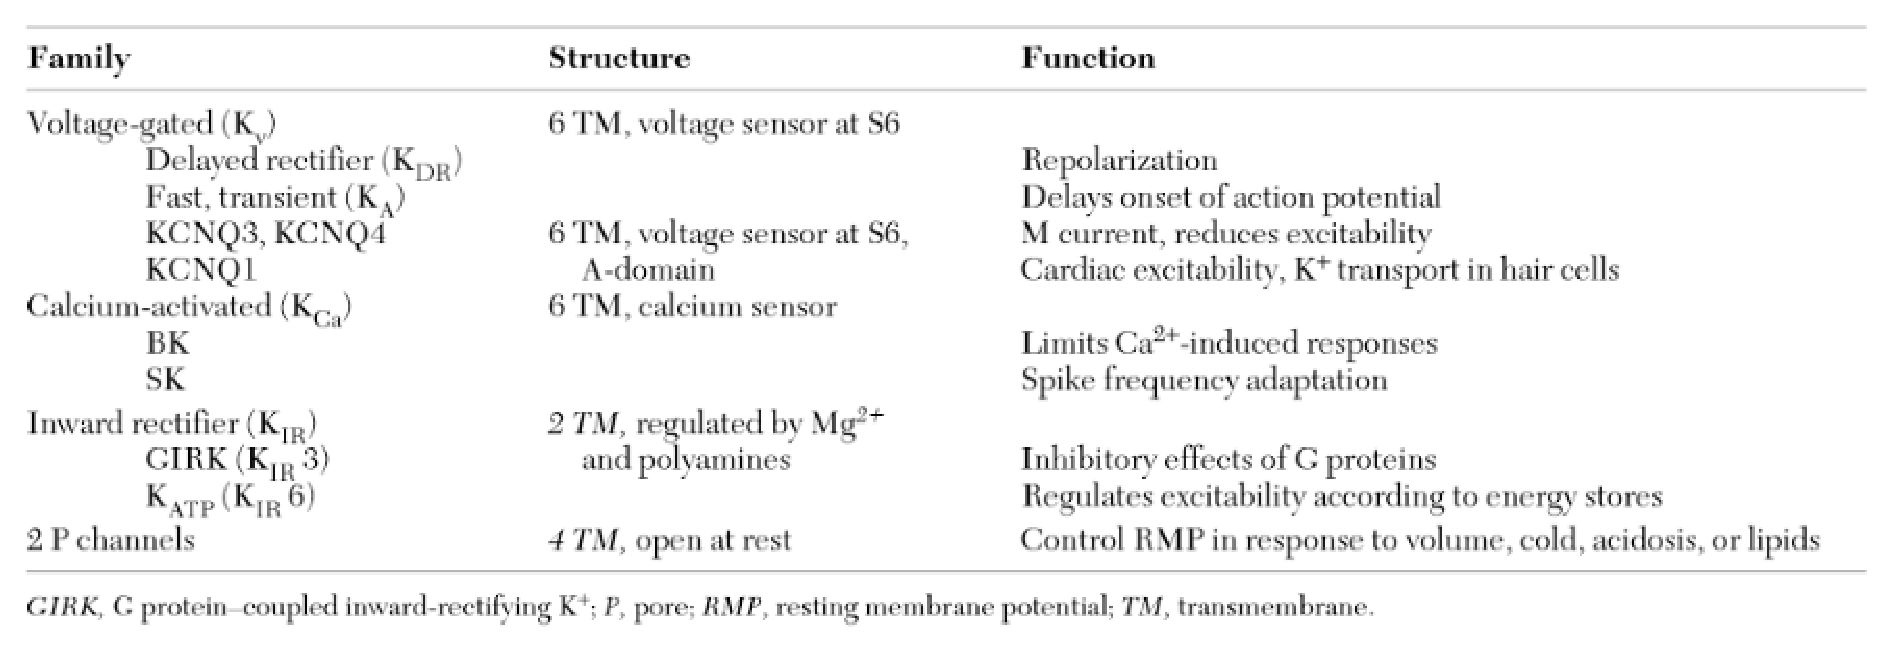
\includegraphics[height=6cm]{./images/K+-channels.eps}}
  \caption{Families of $\K$ channels}
  \label{fig:K+-channel-families}
\end{figure}


% Across the cell membrane, \ce{K+} concentration gradient determines the resting
% potential of the cell. However, this bioelectricity, or electrophysiology, of
% single cells had not been consider adequately until 1950s when the work of
% Hodgkin, Huxley and Katz's and subsequent works showed the permeable of the
% biomembrane to some other ions, \ce{Na+}, \ce{Ca^2+} and \ce{Cl-}... also.

\subsection{based on the number of transmembrane domains}
\label{sec:nomenclature-K_channel-based-number-TM}

A functional K+ channel protein is a tetramer, typically of four identical
subunits.  The genes encoding for a single subunit for potassium channels can be
divided into 8 conserved families, Fig.\ref{fig:K-channel_classification}.
 
\begin{itemize}
  
  \item {\bf 4TM/P}: a novel class of potassium channel, as it only requires 2
  subunits to form a single channel of that class, while the other two requires
  4 subunits.

It should be noted that the more subunits an ion channel is made out of, the
less selective it tends to be to the passage of its respective ion. So, 
potassium channels with two 4TM/P subunits are more selective to $\K$ ions than
the other two structural of potassium channels.

  \item {\bf 2TM/P}: inward-rectifier $\Kir$ family (Sect.\ref{sec:Kir_family}) 

  ($\Ca$-independent) inward-rectifier (anomalous rectifier, KIR or
  $\Kir$) which is gated by different intracellular signals: many subfamilies
  classified into ``weak inward rectifiers'' and ``strong inward rectifiers''.
  
  \item {\bf 6TM/2P}: A subunit is comprised of 4TM/P and 2TM/P. Based on the
  ancillary subunits, the 6TM/P domain superfamily can be dividied into
  conserved gene families
%  $V_m$-gated ($\Kv$) family (Sect.\ref{sec:Kchannel_Vm-dependent}), KQT, Eag
% (Sect.\ref{sec:Eag-like_Kchannel}), Slo ($\Ca$-dependent $\K$ channels family
% - Sect.\ref{sec:Kchannel_Ca-activated}), and SK
  
\begin{enumerate}
  \item Kv channels ($V_m$-gated $\K$ channels) -
  Sect.\ref{sec:Kchannel_Vm-dependent} or Sect.\ref{sec:Kv_channel}
  
  
  \item CNG (HCN channels -  Sect.\ref{sec:HCN-channels}) 

  \item leak $\K$ channels (Sect.\ref{sec:K_leak-current}) 

  \item KCNQ channels (originially known as KvLQT channels)
  
  \item EAG-like $\K$ channels (Sect.\ref{sec:Eag-like_Kchannel})

  \item K(Ca) ($\Ca$-dependent $\K$ channels family
  - Sect.\ref{sec:Kchannel_Ca-activated}):
	\begin{itemize}
	  \item Slo-like channel: BK channel ($I_C$)
	  \item IK channel
	  \item SK channel ($I_\AHP$) - Sect.\ref{sec:SK_current}
	\end{itemize}
\end{enumerate} 
K(Ca) channels are architecturally similar to Kv channels,
with an extra transmembrane segment near the amino terminus
(Sect.\ref{sec:K_regulatory-factors}).

%Each family (Kv, K(Ca), and Kir) are classified into subfamilies. 

  \item {\bf 7TM/2P}: Sect.\ref{sec:MaxiK-current}
  
  \item {\bf 8TM/2P}: hybrids of 6TM/P and 2TM/P, and were first found in yeast
\end{itemize}
%as discussed in Sect.\ref{sec:structure-K-channel}\citep{Miller2000}. 

% Other
% variations in structures will be discussed in
% Sect.\ref{sec:K_channel-nomenclature}.


% \textcolor{red}{The first 2 families of channels allows outward K
%   currents. $\Kir$ are the inward rectifiers}.

% In terms of transmembrane topology, there are 2 broad types,
% Fig.~\ref{fig:K_channel}: 

\subsection{based on homology of hydrophobic TM core}
\label{sec:K+-channel-classification-TM-core}
\label{sec:nomenclature-K_channel-based-homology-TM-core}

Based on the {\it homology of the hydrophobic transmembrane core}, the $\alpha$
subunits are classified into 12 classes ($\Kv$1-12 or $\Kv\alpha$1-12)
\citep{choe2002pcs}.  The $\alpha$-subunits form non-activating Kv channels.

To have fast or slow inactivating properties, ancillary subunits need to be
added to the channel. There's an $\beta$-subunit associated with each
$\alpha$-subunit in some classes (Sect.\ref{sec:Kv-ancillary-subunits}) that
aims to modulate the activity of $\Kv$ channels, rather than conducting current,
e.g. Fig.\ref{fig:MaxiK_channel}.

\textcolor{red}{\bf CLASSIFICATION 1}: based on Kv1-Kv12
\begin{enumerate}

  \item Kv1 \ldots Kv4: Sect.\ref{sec:Kv-Drosophila}


 \item Kv5 \ldots Kv10: Sect.\ref{sec:Kv-non-Drosophila}
\end{enumerate}

% Other than using the homology-based classification described above, we'll
% choose the following classification to describe the $\K$ channels:


\subsection{based on Drosophila genes}
\label{sec:K+-channel-classification-Drosophila-genes}
\label{sec:nomenclature-K_channel-based-Drosophila-genes}


Efforts to isolate cDNA encoding Kv channels $\alpha$ subunits from {\it
Drosophila melanogaster} has lead to the naming based on the gene locus.
There are total four different genes that encode potassium channels in {\it
Drosophila melanogaster}
\begin{enumerate}
  \item Shaker - Sect.\ref{sec:Shaker-gene}
  \item Shab - Sect.\ref{sec:Shab-gene}
  \item Shaw - Sect.\ref{sec:Shaw-gene}
  \item Shal - Sect.\ref{sec:Shal-gene}
\end{enumerate}

\subsection{based on human genes (KCN* genes)}
\label{sec:K+-channel-classification-human-genes}
\label{sec:nomenclature-K_channel-based-Human-genes}

Kv channel $\alpha$ subunit genes start with KCN; then a letter indicating the
gene index; and finally a number indicating the isoform
\begin{enumerate}
  \item KCNA = Kv1: Kv1.1 = KCNA1
  \item KCNB = Kv2
  \item KCNC = Kv3
  \item KCND = Kv4: Kv4.2 = KCND2
\end{enumerate}

\textcolor{red}{CLASSIFICATION 2}: In human, we can classify based on the genes
family of potassium channels, which is known as
KCN\footnote{\url{http://ghr.nlm.nih.gov/geneFamily/kcn}}
\begin{itemize}
  
  \item KCNA: 
\begin{itemize}
  \item KCNA1 = Voltage-gated, Shaker-related family, member 1
  \item KCNA3 = $\Kv$1.3: channels encoded by KCNA3 gene in human (found in T
 and B lymphocytes). Each human T-cell expresses about 300 Kv1.3 and about 10-20
$\Ca$-activated Kca1.3 channels
\end{itemize}

Kv1.1, Kv1.5 and Kv1.6 are encoded by genes on chromosome loci 12p13.

  \item KCNJ

\begin{itemize}
  \item KCNJ2 = Kir of subfamily J, member 2
\end{itemize}

  \item \ldots

%\item KCNJ

  \item KCNQ

\item \ldots
\end{itemize}

\subsection{based on kinetics (i.e. time dependence)}
\label{sec:K+-channel-classification-kinetics}
\label{sec:nomenclature-K_channel-based-kinetics}

By using time dependence as a basis for classification, Kv currents may be
divided into two archetypical categories: slow 'delayed rectifier' currents and
rapid 'A-type' currents.

\textcolor{red}{CLASSIFICATION 3}: The other property of Kv channels 

\begin{enumerate}

  \item A-type currents (I$_A$) - Sect.\ref{sec:A-type-K+current}): rapidly
  inactivating.
  
  Kv1.4, Kv3.x (Kv3.3, Kv3.4), Kv4.x

$I_A$ is encoded by {\it Shal} gene (in neurons), and {\it Shaker} gene (in
muscle) \citep{tsunoda1995}.

  \item delayed rectifier (Sect.\ref{sec:delayed-rectifier})
    (also called non-A-type voltage-dependent K channels) 
    includes Kv1.x, Kv2.x, Kv3.x (Kv3.1, Kv3.2), Kv7.x 
    (Sect.\ref{sec:Kv7.x}) and Kv10.x (Kv10.1, Kv10.2) : delayed onset of
    activation followed by little or slow inactivation (slowly  inactivating or non-inactivating).

The term delayed rectifier was first used by Hodgkin-Huxley to describe the
voltage-dependent K+ current that developed after the Na+ current in response to
depolarization of {\it Loligo } giant axons
(Sect.\ref{sec:Hodgkin-Huxley-1952-model}).

 $\Kdr$ (obsolete symbol $I_\k$, current symbol  $I_\text{K2}$,
 $I_\text{K-DR}$, $I_\text{k,DR}$)

  \item Slowly activating: Kv12.x (Kv12.1, .2, and .3)
  
  \item Outward-rectifying: 
  Kv$\alpha$10.x: Kv10.2 (KCNH5)

  \item Inward-rectifying (Sect.\ref{sec:rectification} - pass current more
  easily into the cell at depolarized potential): Kv11.x (Sect.\ref{sec:Kir_family}).
  
  Kv$\alpha$11.x - ether-a-go-go potassium channels: Kv11.1 (KCNH2) - hERG,
  Kv11.2 (KCNH6), Kv11.3 (KCNH7)
  
  
   \textcolor{blue}{The total $V_m$-dependent outward $\K$ current in most neurons
and muscles can loosely be accounted by the two components}: rapidly
inactivating A-current $I_A$ (time constant $\tau_h\approx 10$ms), and the
slowly inactivating ``delayed rectifier'' component $I_{K2}$ (or $I_\Kdr$)
($\tau_h=200-2000$ms). Each can also be subdivided into subtypes, e.g. $I_{A1},
I_{A2}, I_{K2a}, I_{K2b}$, to fit to activation and inactivation curves with
different time constant \citep{huguenard1992}. 

  \item K(Ca) class (Sect.\ref{sec:Kchannel_Ca-activated}):
  Maxi-$K_\ca$ channels (Sect.\ref{sec:MaxiK-current}) 
  
\end{enumerate}
%\url{http://en.wikipedia.org/wiki/Voltage-gated_potassium_channel#A-type_potassium_channel}

\section{Two-pore-domains channel (K2P): 4TM/2P}
\label{sec:K2P}
\label{sec:tandem-pore-domain-K+-channel}

Before 1995, K+ channel subunits were identifiable by the presence of a single
pore-forming P domain. The identification of $\K$ channels with two-pore domains
in tandem was predicted in 1995 for the TOK1 (YORK). However, this yeast channel
possessed 8TM; and it was strongly outward rectifying (Sect.\ref{sec:TOK}).

The $\KtwoP$ channels are mainly dimers (homodimers), with a pseudo-tetrameric
pore (Brohawn et al., 2012, 2013; Dong et al., 2015; Miller and Long, 2012); 
only a few examples of heteromerization have been previously reported.
\begin{enumerate}
  \item heterologous coexpression of TREK-1 and TREK-2 subunits results in the
  formation of functional heterodimers (Lengyel et al., 2016)
  
The heteromer was inhibited by extracellular acidification and by spadin
similarly to TREK-1. Its ruthenium red sensitivity was intermediate
between TREK-1 and TREK-2 homodimers.

 Formation of TREK-1/TREK-2 channels was also demonstrated in native dorsal root
ganglion neurons indicating that heterodimerization may provide greater
diversity of leak K+ conductances also in native tissues.  
\item 
  \item 
\end{enumerate}

There are at least 42 potential genes for 4TM/2P subunits in the complete
genomic sequence of the nematode {\it Caenorhabditis elegans}, with at least 14
of them have been cloned, studied and formally designated.

Two-pore domain (K2P, tandem-pore, K$_\text{2P}$) family gives rise to leak
(i.e. background) $\K$ current. The current is important in stabilizing the
negative resting membrane potential and counterbalance depolarization.
In 1996, the identification of TWIK (now called TWIK-1) gave birth to this last,
but rapidly emerging family of mammalian background $\K$ channel
(Sect.\ref{sec:TWIK-1-channel}). Now the members are classified into different
subfamilies (Sect.\ref{sec:K2P-classification}).


\begin{mdframed}

REMINDER: There are three major families of K+ channel (review: O'Connell et
al., 2002).:
\begin{enumerate}
  
  \item voltage-gated family (Kv - Sect.\ref{sec:Kv_channel}), including K(Ca) -
  Sect.\ref{sec:Kchannel_Ca-activated}),

  \item inward rectifier family (Kir - Sect.\ref{sec:Kir_family}) and 
  
  \item two-pore domain (this section).
% As all functional K+ channels are thought to have four P-domains; thus K2P
% channels would comprise two subunits.
\end{enumerate}

\end{mdframed}

We will split into two parts
\begin{enumerate}
    \item KCNK - in animal (mammalian, and yeast) - Sect.\ref{sec:KCNK}
    \item KCO1 - in higher plant - Sect.\ref{sec:KCO1}
\end{enumerate}

\subsection{K2P classification}
\label{sec:K2P-classification}

\begin{figure}[hbt]
  \centerline{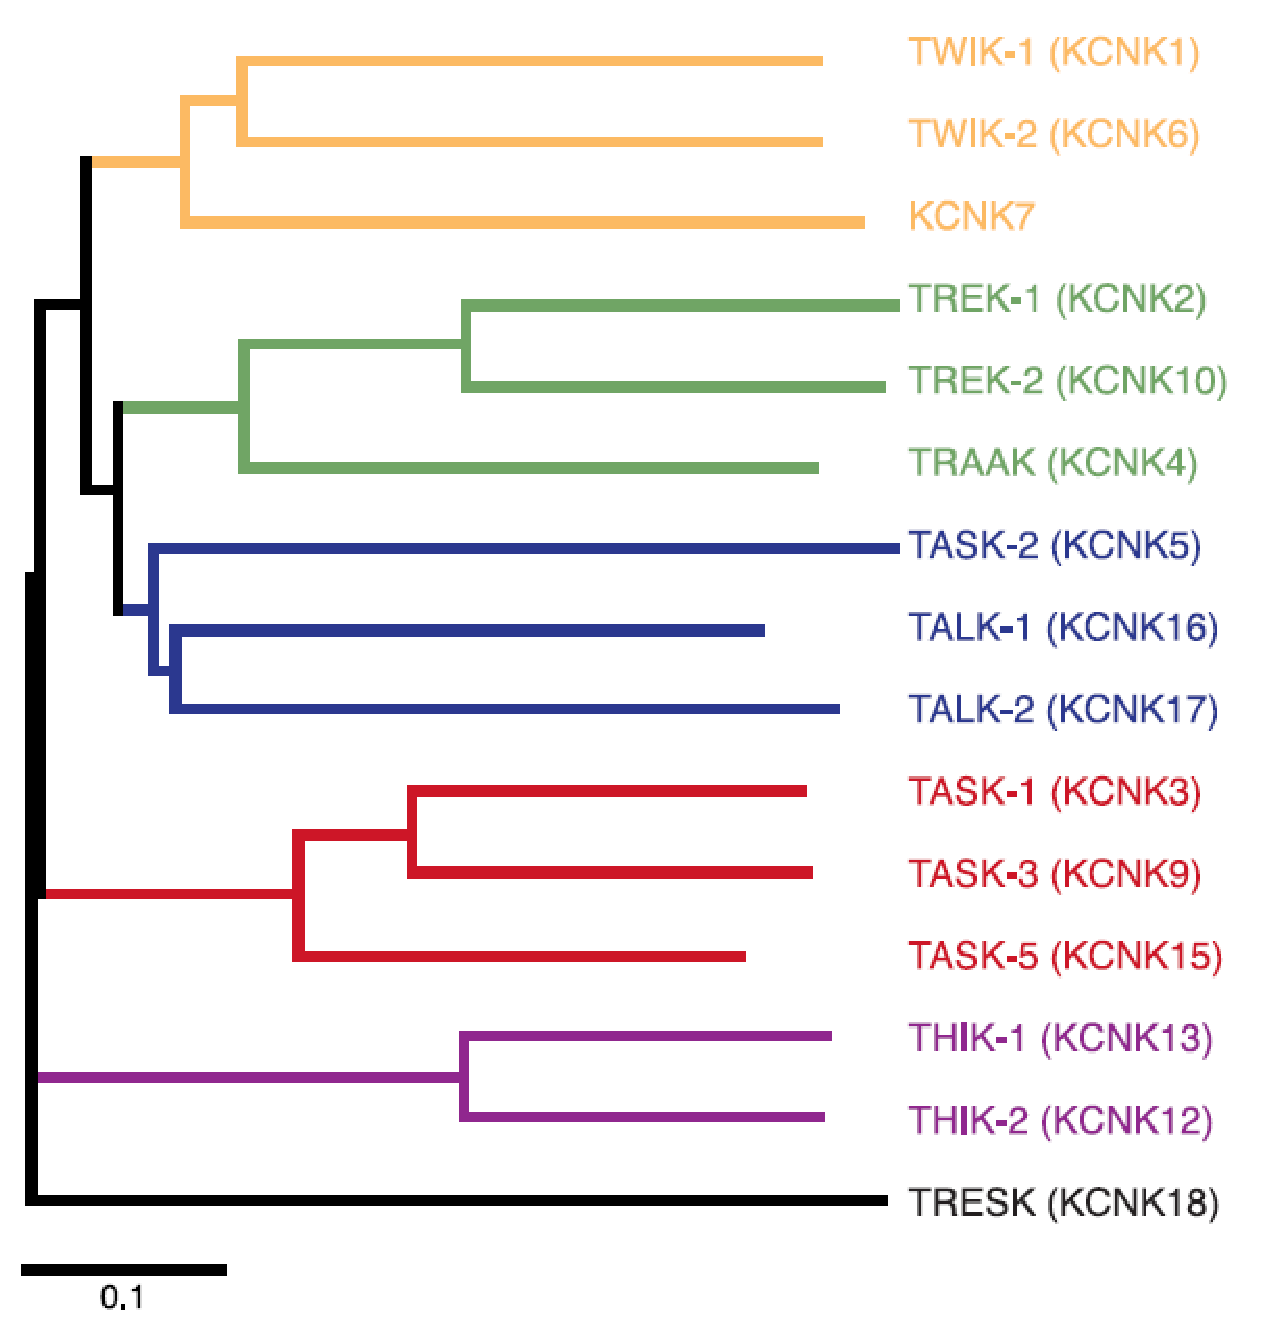
\includegraphics[height=5cm,
    angle=0]{./images/K2P_classification.eps}}
  \caption{NOTE: KCNK8, KCNK11, and KCNK14 do not exist.}
\label{fig:K2P_classification}
\end{figure}

The 15 members of human $\KtwoP$ can be divided into 6 subfamilies based on
sequence similarities and functional resemblance, Fig.\ref{fig:K2P_classification}
\begin{enumerate}
  \item TWIK - Sect.\ref{sec:TWIK-channel}
  
  \item TREK - Sect.\ref{sec:TREK-channel}: TREK-1 and TREK-2
  
  \item TASK - Sect.\ref{sec:TASK-channel}
  
  \item TALK - Sect.\ref{sec:TALK-subfamily}
  
  \item THIK
  
  \item TRESK
\end{enumerate}

\subsection{1. Leak potassium currents (KCNK, dORK)}
\label{sec:leak-K+-current}
% \subsection{Leak $\K$ current (KCNK or K2P)}
\label{sec:K_leak-current}
\label{sec:dORK}
\label{sec:KCNK}

Leak currents have been described since 1950s.
We now understand that leak is not just seepage, but flux through dedicated
pathways.

In this section, we describe $\KtwoP$ channels in mammalian and yeast. For
higher plant, check Sect.\ref{sec:KCO1}.
The name K2P (or $\KtwoP$) is derived from the fact that the alpha subunits has
two pore regions - {\bf two-pore-domain} (tandem-pore or two-P-domain).

Two-pore-domain $\K$ channels are substrate for resting $\K$ currents in
neurons. The name KCNK is the animal homologue of K2P with four $\alpha$
subunits, each  of 4 TM and two pore-loop (2P) - Sect.\ref{sec:4TM/P}.

KCNK was first called {\bf dORK} channel as the first type - KCNK0
(Sect.\ref{sec:KCNK0}) - was first found in {\it D. melanogaster} neuromuscular
gene library (as {\it kcnk}$\Theta$ gene for KCNK$\Theta$ channel) and operate
as openly rectifying with $\K$ selective leak pore. Although KCNK channels were
discovered recently, since 1996, they outnumbered other channel types (Goldstein
et al., 1996; Ilan and Goldstein, 2001) - Sect.\ref{sec:KCNK-classification}).

K2P channels, along with some other channels that operate at resting membrane
potential (Sect.\ref{sec:resting-membrane-potential}), are responsible for
baseline or leak currents (Sect.\ref{sec:leak-current}).

Example:
\begin{enumerate}
  \item marine snails Aplysia : the serotonin-sensitive S-type background K+
  channels
  
  synaptic sensitization down-modulate this serotonin-sensitive S-type K+
  current.
  
  \item marine snails Lymnaea: the anaesthetic-sensitive background K(An)
  channels - Sect.\ref{sec:TASK1}
  
 stimulation of K(An) channels can hyperpolarize and reversibly suppresses
 electrical activity in anaesthetic-sensitive pacemaker neurons.

\end{enumerate}

\subsection{-- functions}

The well know function of background $\K$ current is to stabilize the negative
resting membrane potential and counterbalance depolarization.

\begin{itemize}
  
  \item  In neurons, they are a major determinant not only of membrane potential
  but also membrane input resistance, which is a primary factor in the magnitude
  and kinetics of responses to synaptic inputs.

  \item  Current flow through K2P channels is determined predominantly by the
  prevailing electrochemical gradient for K+, and

  \item The I/V curves (Sect.\ref{sec:I-V-curve}) can be described by the GHK
  equation (GHK rectification or open rectification -
  eq.\ref{eq:GHK-current}), i.e. possess Goldman-Hodgkin-Katz (open)
  rectification (Sect.\ref{sec:rectification}), i.e. non-linear potassium leak.
  
  \item  Given the normal concentration gradients, with high K+ inside and low
  K+ outside the cell, outward currents are larger than inward currents because
  of the availability of ions. This appears as an outward rectification of the
  currents that disappears if the external K+ concentration is raised to
  cytosolic levels (Sect.\ref{sec:rectification}).
\end{itemize}

\subsection{-- kinetics}

As the open probability is independent of voltage, thus, these channels are
thought to contribute to the resting membrane potential and are classified as
background K+ channels. Previously, it is assumed that the current via the
background $\K$ channel is passive, i.e. I=g*(V-E).

However, it is now known that this primary hyperpolarizing action is not
performed passively. These channels are regulated by several voltage-independent
mechanisms including oxygen tension, pH, mechanical stretch, and G-proteins
(Sect.\ref{sec:G-protein}). 

For models, read Sect.\ref{sec:leak-K+-current-models}.

% ``Leak'' $\K$ current, aka {\bf tandem pore domain $\K$ channels} (or two pore
% domain potassium - K2P) is a family of 15 members. 

\subsection{-- agonists: 2-APB}
\label{sec:2-APB}

K2P channels are generally sensitive to anaesthetics, and usually show
differential sensitivity to inhalation (e.g., halothane, isoflurane) and local
(e.g., lidocaine, bupivicaine) agent (review: O'Connell, Hunter, 2002).

2-Aminoethoxydiphenyl borate (2-APB) has been recently identified as a common
agonist of TWIK-related K(+) channel (TREK)/TRAAK channels, a subfamily of
two-pore domain K(+) (K2P) channel.

However, TREK-2 displays much higher sensitivity to 2-APB compared with TREK-1,
despite that these two channels share the highest homology among K2P members
(Zhuo et al., 2015).

% Insights into the stimulatory mechanism of 2-aminoethoxydiphenyl borate on
% TREK-2 potassium channel.
% R-G Zhuo, X-Y Liu, +4 authors X-Y MaNeuroscience2015


\subsection{KCNK classification}
\label{sec:KCNK-classification}

K2P is a family of 15 members (K$_\text{2p}$x.y) form what is
known as "leak channels". 
\begin{itemize}
  \item {\it D. melanogaster} has 11 {\it kcnk} genes
  
  \item {\it C. elegans}: over 50 putative K2P channels in {\it C.
  elegans}, which is about half of the total K2P channels in animal's genes
  (review: \citep{OConnell2002}).

  \item   There are 7 two-pore-domain $\K$ channels in rat and mouse

The nomenclature is quite confusing. NOTE: There are genes of multiple names,
e.g. Kcnk6 is officially Kcnk8. However, Kcnk8 should have been Kcnk7, as {\it
Kcnk8 is the mouse variant of the human gene KCNK7}. There are also subunits
named for functional attributes that later proved to be minor or inaccurately
assessed.
 
\end{itemize}


Because of the confusing in naming, a simplified terminology that is gene-based
is recommended to use and in accord with HUGO (Human Genome Organization)
assignations; for example, 
\begin{itemize}
  \item  {\it KCNK0} gene (in italic) and KCNK0 channel
  \item {\bf $\KtwoP1-18$} for protein products.
\end{itemize}
On mammals, we focus on 7 of them from KCNK1 to KCNK5, KCNK9, and KCNK10
\citep{talley2001}, Fig.\ref{fig:K2P_classification}.

\begin{itemize}
  \item KCNK0 = dORK1
  
  \item KCNK1 = K$_{2p}$1.1 = TWIK-1 - Sect.\ref{sec:TWIK-1-channel} 
  
  
  \item KCNK2 = TREK-1 (Sect.\ref{sec:TREK-1-channel})
  
  \item TASK family: Sect.\ref{sec:TASK-channel}
  \begin{enumerate}
    \item KCNK3 =   K$_{2p}$3.1 = TASK-1, 

    \item KCNK5 = K$_{2p}$5.1 = TASK-2, 
    
    \item KCNK9 = K$_{2p}$9.1 = TASK-3, 

    
    \item K$_{2p}$17.1 = TASK-4,
     
    \item K$_{2p}$15.1 = TASK-5
  \end{enumerate}
   
  \item KCNK4 = K$_{2p}$4.1 = TRAAK (Sect.\ref{sec:TRAAK-channel})
  
%  mRNA for TRAAK also was highest in the cortex
  
  
  \item K$_{2p}$7.1
  
  NOTE: There is no channel name K$_{2p}$8.1, K$_{2p}$11.1 and K$_{2p}$14.1.
  
  \item K$_{2p}$9.1 
  
  \item KCNK10 = K$_{2p}$10.1 = TREK-2  (Sect.\ref{sec:TREK-2-channel})
  
%  expression of TREK-2 was primarily restricted to   the cerebellar granule
  % cell layer.
  
  \item \ldots
  \item K$_{2p}$15.1 =
  \item \ldots 
  \item K$_{2p}$18.1 
\end{itemize}
 
The differential expression of each of these genes likely contributes to
characteristic  excitability  properties  in  distinct  populations  of
neurons,  as  well  as  to  diversity  in  their  susceptibility  to
modulation.
\footnote{\url{http://en.wikipedia.org/wiki/Tandem_pore_domain_potassium_channel}}


There are two particular processes regarding K2P channel trafficking
for which most evidence exists.
\begin{itemize}
  \item TASK channel trafficking from ER
  \item TREK channels localized to particular regions in neuronal membrane.
\end{itemize}

\subsection{-- KCNK0 (dORK1)}
\label{sec:KCNK0}

KCNK0 is the first background $\K$ channel cloned (from {\it Drosophila
melanogaster}) in 1996. Initially, it was named dORK1 (or ORK1, d=drosophila),
and later was renamed to KCNK0 by the author when more members of background
potassium channels are found.

\textcolor{red}{Kinetics}
\begin{enumerate}

  \item macroscopic current is instantaneous, independent of voltage and
  selective for K+.

  \item  showed a behaviour called 'Goldman-Hodgkin-Katz rectification' or 'open
  rectification', as their conduction properties approximated predictions of
  constant-field current equations for free electrodiffusion through an open
  ion-selective pore (Sect.\ref{sec:GHK-rectification})

  \item Whereas all KCNK channels are expected to leak in this fashion, the
  various isolates have already begun to reveal their individual differences.

  \item  \textcolor{red}{IMPORTANT: studies of single KCNK0 channels have shown
  that leak channels are not always open}, depending upon protein kinase action:
  when kinases are active (open probability, Po $\approx$ 1) and close when they
  are suppressed (Po <0.05).

KCNK0 activity is finely tuned through integration of signals from multiple
second-messenger pathways that involve protein kinases A, C and G.

  \item Notable influences include kinase-dependent pathways, arachidonic acid,
  membrane stretch, external pH and temperature.

\end{enumerate}

\subsection{-- TWIK subfamily}
\label{sec:TWIK-channel}

TWIK means {\bf T}wo pore domain {\bf W}eak {\bf I}nward rectifying K+ channel.

\subsection{---- KCNK1 = TWIK-1 = K2P 1.1 (HOHO1)}
\label{sec:TWIK-1-channel}
\label{sec:KCNK1}
\label{sec:HOHO1}

TWIK-1 (KCNK1) is a weak inward rectifier $\K$ channel
(Sect.\ref{sec:TWIK-channel}).
Human TWIK-1 is also called HOHO1.
Despite high injection of TWIK-1 mRNA, only a small current was detected on {\it
Xenopus laevis} oocytes.

There was widespread distribution of  TWIK-1,  with  highest  levels  in  the
cerebellar  granule  cell layer, thalamic reticular nucleus, and piriform
cortex. TWIK-1 is also a highly expressed astrocytic K2P, beside TREK-1.

In astrocytes, the major distribution of TWIK-1 is in intracellular
compartments, and if in the membrane, it is a non-selective cation channel (Wang
et al., 2013, 2015).

\begin{itemize}
  \item mGluR3 (Sect.\ref{sec:mGluR_group-2}) activation recruits TWIK-1 channel
  to membrane (Wang et al., 2015).
  
% Wang, W.,Kiyoshi,C.M.,Du,Y.,Ma,B.,Alford,C.C.,Chen,H.,etal.(2015).
% mGluR3 activationrecruitscytoplasmicTWIK-1channelstomembranethat
% enhances ammoniumuptakeinhippocampalastrocytes. Mol. Neurobiol.
% doi: 10.1007/s12035-015-9496-4[Epubaheadofprint].

% Wang, W.,Putra,A.,Schools,G.P.,Ma,B.,Chen,H.,Kaczmarek,L.K.,etal.
% (2013). ThecontributionofTWIK-1channelstoastrocyteK(+)currentis
% limited byretentioninintracellularcompartments. Front. Cell.Neurosci. 7:246.
% doi: 10.3389/fncel.2013.00246

  \item  In another hypothesis, the channel is inserted into the membrane, but
  is silent by a special post-translational modification: sumoylation, by SUMO
  protein.
\end{itemize}
% However, \textcolor{blue}{TWIK-1 is mainly located in intracellular
% compartments}, and its transfer to plasma membrane is tightly regulated. 

{\bf Kinetics}
\begin{enumerate}
  \item at symmetrical $[\K]$: TWIK-1 single channel conductance was 34 pS (at
  -80 mV of symmetrical 140 mM $[\K]$)
  
The same conductance was measured in mutated form, i.e. K274E of human TWIK-1.

  \item TWIK-1 is mediated by intracellular pH (i.e. blocked by acidification)
  and is activated by PMA - a pharmacological activator of PKC -
  Sect.\ref{sec:PKC} though PMA has no direct effect on TWIK-1.
  
PMA = of phorbol 12-myristate 13-acetate

\end{enumerate}

\subsection{---- KCNK6 = TWIK-2 = K2P 6.1 (TOSS)}
\label{sec:TWIK-2-channel}
\label{sec:KCNK6}

Human or mouse TWIK-2 is also called {\bf TOSS}.

{\bf Kinetics}: kinetics of TWIK-2 was found to be the same as that of TWIK-1
(Sect.\ref{sec:TWIK-1-channel})
\begin{itemize}
  \item TWIK-2 induces a weakly inward rectifying current in symmetrical $[\K]$

The current deviate from an ideal background $\K$ current
(Sect.\ref{sec:leak-K+-current-ideal})
was the activity is a function of $\Vm$ with about 50\% of TWIK-2 inactivate
slowly ($\tau \approx 2$ seconds) at strong depolarization; with steady-state
half-inactivation is at +65 mV; the remaining show ideal background current.

The inactivation is a function of $[\K]_o$, with no inactivation is found in
symmetrical high $[\K]$.
 
  \item human TWIK-2 when expressed in {\it Xenopus} oocytes has a small current
  amplitude:
  $< 0.5 - 1.0 \muA$ in 115 mM $[\K]$ at -100 mV
  
  \item rat TWIK-2 produce 15x higher conductance than human TWIK-2 in COS-7
  cells
  
\end{itemize}


\subsection{---- KCNK7}
\label{sec:KCNK7}

KCNK7 is the third member of TWIK subfamily; yet it cannot be expressed in {\it
Xenopus} oocytes or COS-7 cells. 

NOTE: KCNK7 of different species was initially called as KCNK6 or KCNK8. Later
KCNK6 was renamed to TWIK-2 (Sect.\ref{sec:TWIK-2-channel}) and KCNK8 was
omitted.

Human KCNK7 has an unconventional sequence - GLE - in the second channel pore
domain; while in other channels, the second glycine is strictly conserved, i.e.
GLG, GYG, or GFG - which is important in forming selectivity filter. So, this
raised the question whether KCNK7 may function as a $\K$ channel at all
(Enyedi, Crijak, 2010).

\subsection{-- TREK subfamily}
\label{sec:TREK-channel}
  
TREK means {\bf T}WIK-{\bf R}elated $\K$ channel -
Sect.\ref{sec:TWIK-channel}.
\begin{enumerate}
  \item TREK-1 = KCNK2 = TPKC1
  
  \item TREK-2 = KCNK10
\end{enumerate}

\subsection{---- KCNK2 (TREK-1) = K2P 2}
\label{sec:KCNK2}
\label{sec:TREK-1-channel}

TREK-1 (or KCNK2) is the first member of TREK subfamily
(Sect.\ref{sec:TREK-channel}) and was discovered in Michel Lazdunki's Lab (Fink
et al., 1996). The channel's name has been used rom TPKC-1; then TREK-1; and now
KCNK2. The behavior of the channel is quite complicated (see below).

It is recommended to know KCNK0 first (Sect.\ref{sec:KCNK0}).
TREK-1 and TWIK-1 has low sequence similarity (28\%). Currents generated by
TWIK-1 is inward, yet currents generated by TREK-1 is outward rectifying.

Rat KCNK2 was cloned and found to share 95\% identity with the human gene at
amino acid level. Human KCNK2 gene encodes 426-residue KCNK2 channel subunit.

\textcolor{red}{Regulators}: TREK-1 is highly dynamic and subject to regulation
by various changes occurring in the interstitial environment, such as pH,
temperature, osmolarity, and mechanic force (Patel et al., 1998; Maingret et
al., 1999; Lesage and Lazdunski, 2000; Chemin et al., 2005; Murbartian et al.,
2005).
%  whole-cell TREK-1 currents are
% increased by arachidonic acid, mechanical stretch and volatile anaesthetics and
% diminished by lowered temperature via a protein kinase A (PKA)-dependent
% pathway.
\begin{itemize}
  \item stretch-activated (Fink et al., 1996)

   \item anesthetic-activated:  TREK-1 is also activated by volatile anesthetics
   and has been suggested to be an important target in the action of these
   drugs.
  
  \item heat-activated (Maingret et al., 2000) via PKA-dependent pathway
  
TREK-1 has a seven-fold increase in current accompanies a 10 $^\circ$C increase
in temperature, compared to a two-fold increase in TASK-1 current
(Sect.\ref{sec:TASK1}).

Heat-sensitivity is removed by intracellular cyclic adenosine monophosphate
(cAMP), and by mutation of serine (S) at position 333 to alanine.
As serine is a site for phosphorylation by protein kinase A.

   \item PKA phosphorylation at serine site: 
   
   TREK-1 changes from a leak channel to a voltage-gated channel upon
   phosphorylation of S333.
   
 
   \item  TREK-1 is inhibited by neurotransmitters that produce an increase in
intracellular cAMP (Sect.\ref{sec:cAMP}), e.g. cholinergic modulation, and by
those that activate the Gq protein pathway (Sect.\ref{sec:Gq/11-protein}).

  \item internally applied arachidonic acid and polyunsaturated fats can
  stimulate TREK-1; similar to TREK-2 and TRAAK (Sect.\ref{sec:TRAAK-channel})

\end{itemize}

{\bf Kinetics}: the kinetics deviate from ideal background $\K$ current because
of 2 factors: (1) a function of extracellular $[\K]_o$ and $[\Ca]_o$; (2)
voltage-dependency. TREK-1 is an outwardly rectifying leak type
K+ channel that follows Goldman-Hodgkin-Katz (GHK) constant field rectification
(Fink et al., 1996). 

IMPORTANT: The GHK equation also anticipates that leak channels lack voltage
and time dependency - that is, K+ flow should remain stable over time. However,
several mammalian K2P channels, including TREK1, show both voltage- and
time-dependent gating.


\begin{enumerate}
	
    \item current - voltage relationship of the potassium leak conductance
   deviates significantly from a linear ohmic leak due to the asymmetrical
   distribution of potassium ions across the membrane.

	In the symmetrical case of $[\K]$: the single-channel current 
	is linear or slightly inwardly rectifying, which can be modeled as an ideal
	background $\K$ current (Sect.\ref{sec:leak-K+-current-ideal}).
	
	However, in the presence of physiological concentration of $\K$ and $\Ca$, the
	unitary conductance of TREK-1 is progressively reduced at negative $\Vm$ and
	has a tendency to saturate at very negative $\Vm$. Because of this, it produces
	a marked {\bf outward rectification}, which opposite the electrical driving
	force to create this saturation. The conductance is however, in sensitive to
	$[\Mg]_o$.
	
	The outward rectification is attributed to external $[\Mg]_o$ block which is
	present at negative $\Vm$; and to an intrinsic voltage-dependent mechanism
	(review: Honore (2007)).
	
	\item TREK-1 opening probability $P_o$ can be as high as 0.6  at high positive
	$\Vm$.

Early reports described TREK-2 as a non-voltage gated K+ outward rectifier (i.e.
almost instantaneous activating channel); however, it is later revealed that it
is also accompanied by a fast ($\tau = 4 - 6$ ms) time-dependent component,
representing the Vm-gated property. 

   \item TREK-1 does not inactivate; with a low deactivation time $\tau = 5 - 7$
   ms. 

This fast activation and deactivation may explained why Vm-depedenty property
was not detected in certain voltage-clamp protocols.

  \item TREK-1 expressed in mammalian cells exhibits small ( approximately 52
  pS) and large ( approximately 220 pS) unitary conductance levels
  
  At symmetrical $[\K]$ of 140 mM: the single channel conductance is 95-130 pS
  at positive $\Vm$. The channel can also exihibit low conductance, 40 pS,
  with shorter splice variants.
  
  \item  TREK-1 is an open rectifier when the single canonical PKA consensus
site is mutated to alanine (or bears no phosphate), passing
large currents both inwards and outwards in symmetrical
conditions.
  
  \item If the PKA consensus site is altered to aspartate (or phosphorylated)
  it passes more outward current even in symmetrical K+ owing to
  voltage-dependent changes in their open probability 
  
  \item half-maximal activation voltage value is >0 mV and it does not change
  with EK
  
This phenotypic alchemy is expected to enhance neuronal excitability as leak
currents inhibit depolarization towards firing threshold, whereas channels
activated at supra-threshold potentials do not interfere with rise to threshold
but do facilitate recovery and repetitive re-firing.


\end{enumerate}


TREK-1 is expressed robustly in the central nervous system (CNS), especially in
the hippocampus (Bockenhauer et al., 2001),
\begin{enumerate}

  \item TREK-1 was highest in the striatum and in parts of the cortex (layer IV)
  and hippocampus (CA2 pyramidal neurons). 

  \item TREK-1 is highly expressed in (hippocampal) astrocytes.
  
  TREK-1 proteins were mainly located in the intracellular compartments of the
  hippocampus. Covalent association of TREK-1 with TWIK-1
  (Sect.\ref{sec:TWIK-1-channel}), has been reported as a mechanism underlying
  the  trafficking of heterodimer TWIK-1/TREK-1 channel to the membrane and 
  contributing astrocytic passive conductance. However, in a nother study, Du et
  al. (2016) don't see any change to electrophysiological properties of the
  astrocyte.
  %http://journal.frontiersin.org/article/10.3389/fncel.2016.00013/full
% and contributing to astrocyte passive conductance.


\end{enumerate}


TREK-1 has an important role in neuroprotection against epilepsy and brain and
spinal chord ischemia. In particular, Trek1-/- mice display an increased
sensitivity to ischemia and epilepsy.

\subsection{---- KCNK10 (TREK-2)}
\label{sec:TREK-2-channel}
\label{sec:KCNK10}

Expression of TREK-2 was primarily restricted to the cerebellar granule cell
layer.  \url{http://www.jneurosci.org/content/21/19/7491.short}
 
{\bf Kinetics}:
\begin{enumerate}
  \item The $P_o$ at +40 mV is about 2x as high as that at -40 mV.
  
  \item in constrast to TREK-1, depolarization actually decreases the
  conductance of TREK-2.
  
This inward rectification of the unitary current may balance the voltage-driving
force, and resulting in an almost linear and only slightly outward rectifying
current in symmetrical concentration case.

  \item 
\end{enumerate}

\subsection{---- TRAAK current: KCNK4, K2P 4}
\label{sec:TRAAK-channel}
\label{sec:KCNK4}

TRAAK is {\bf T}WIK-{\bf R}elated {\bf A}rachidonic {\bf A}cid-activated $\K$
channel, and is a member of TREK subfamily (Sect.\ref{sec:TREK-channel}). mRNA
for TRAAK also was highest in the cortex

{\bf Kinetics}
\begin{enumerate}
  \item internally applied arachidonic acid and polyunsaturated fats can
  stimulate TRAAK, similar to TREK-1 and TREK-2.

  \item the TRAAK current is not affected by $[\Mg]_o$
  
  \item single channel I-V relationship is only slightly inward, under
  symmetrical $[\K]$
  
  \item in physiological concentration $[\K]$, the conductance is 45 pS in the
  range of $\Vm$ [0, +60] mV. 
  
  \item at whole-cell level, TRAAK has a classical non-rectifying leak channel
\end{enumerate}

\subsection{-- TASK subfamily}
\label{sec:TASK-channel}
\label{sec:pH-sensitive-K+-channel}
\label{sec:K+-channel-pH-sensitive}

TASK is {\bf T}WIK-related with (extracellular) {\bf A}cid-{\bf S}ensitive $\K$
channel in the physiological range, and was first cloned from kidney.
As the name implies, these channel are sensitive to pH levels.

The biological mechanism for pH-sensitivity may link to histidine residue at
distal to the P domain (in TASK-1 and TASK-3) because the mutation of this
residue, e.g. H98N, causes a large reduction in pH-sensitivity. The inhibition
by protons (\ce{H^+}) is voltage-independent; and protons do not enter the filter pore to
block the channel; instead it exerts the inhibition by titration an amino acid
on the extracellular side.

\begin{enumerate}
  \item TASK1 (TBAK1, OAT1, KCNK3) - Sect.\ref{sec:TASK1}  
  
  \item TASK3 (KCNK9) - Sect.\ref{sec:TASK3}
  
  \item TASK5
\end{enumerate}

IMPORTANT: Despite having names with TASK, the two channels below do not belong
to TASK subfamily
\begin{itemize}
  \item TASK2 (KCNK5) - Sect.\ref{sec:TASK2}
    
  \item TASK4 - Sect.\ref{sec:TASK4}
\end{itemize}

Among file of them, only four are functional TASK channels (TASK-5 is
nonfunctional) and they have different sensitivities to extracellular pH. These
channels show currents as a function of extracellular pH, i.e. [H+].
% \begin{equation}
% \frac{I}{I_\max} = \frac{1}{1 + \left( \frac{[\H]}{K_D} \right)^n}
% \end{equation}
The formula
\begin{equation}
I = I_\max \times \frac{1}{1 + \left(\frac{[\H]}{K_D}\right)^n}
\end{equation}
with $[\H]$ is hydrogen ion concentration. 

As shown in the table below, only TASK-1 and TASK-2 are influenced by
extracellular pH under normal physiological condition (check Figure 3,
O'Connell, Hunter (2002)). Thus, the physiological relevance of TASK-4 is not
cleared, even though co-expression of TASK-4 with other channel subunits may
alter its pH-sensitivity.

\begin{verbatim}
              Kd      n (Hill coefficient)
TASK-1        7.3     1.5
TASK-2        8.3     0.7
TASK-3        6.7     2.0
TASK-4        10      1.0
\end{verbatim}


\begin{itemize}
  \item TASK channels do exhibit some TEA sensitivity (IC50 = 10 mM) (Brickley
  et al., 2007)
  
  \item  It seems from these curves that only TASK-1 and TASK-2 have pK's which would
allow regulation by the extracellular pH under normal physiological conditions.
The low pK of TASK-3 would suggest that it would be permanently open, but it is
expressed in the stomach where the lumen pH is around 4.5 and the pH in the
gastric pits themselves may be less than one.

  \item TASK-4 has an extremely alkaline pK, and is expressed, amongst other places
(liver, lung, placenta, pancreas, small intestine, aorta, heart atrium, colon,
ovary, peripheral blood leukocytes, prostate, spleen, testis and thymus, small
extent in brain), in the pancreas where the pH within the lumen of the secretory
ducts is approximately 0.5 pH units alkaline to plasma. The physiological role
of TASK-4 is unclear; though its coexpression with other channel subunits may
change its pH sensitivity.
  
  \item 
\end{itemize}

TASK-1 (Sect.\ref{sec:TASK1}) and TASK-3 (Sect.\ref{sec:TASK3}) mRNA transcripts
are found in neural tissue, while TASK-2 is highly expressed in the kidney, and
TASK-4 is ubiquitously expressed, but to a lesser extent in neural tissue
\citep{OConnell2002}.

For  TASK-1,  highest  mRNA accumulation  was  seen  in  the  cerebellum  and 
somatic  motoneurons. 

TASK-3  was  much  more  widely  distributed,  with robust  expression  in  all 
brain  regions,  with  particularly  high expression  in  somatic  motoneurons, 
cerebellar  granule  neurons, the locus ceruleus, and raphe nuclei and in
various nuclei of the hypothalamus.


\subsection{---- KCNK3 (TBAK1, TASK1, OAT1 and KCNK3): background current
in neurons and hearts}
\label{sec:KCNK3}
\label{sec:TASK1}
\label{sec:OAT1}
\label{sec:TBAK1}

There are identical subunits with multiple names; for example, TBAK1,
TASK1, OAT1 and KCNK3 are the same subunit.

TASK-1 is found in cerebellar granule neurons (CGNs -
Sect.\ref{sec:granule_cells}). Under genetic ablation, the AP in CGN neuron has
a significantly broader and smaller AP.  Similar observation also found in
orexin/hypocretin neurons and cardiac tissues (review: MacKenzi et al., 2015).
  
\begin{figure}[hbt]
  \centerline{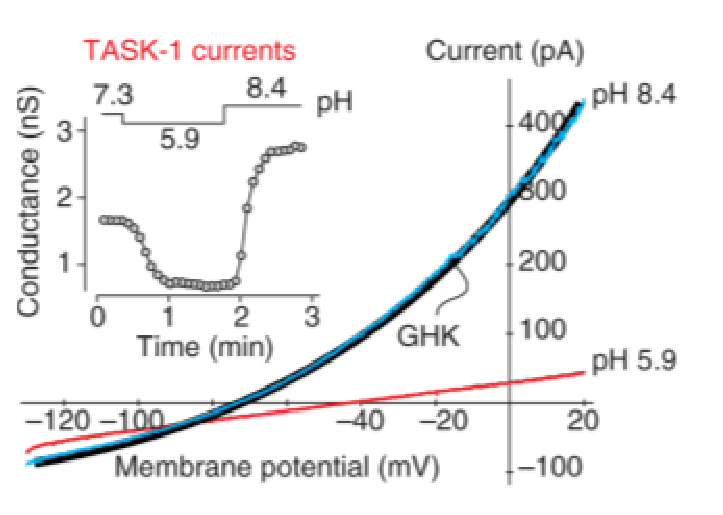
\includegraphics[height=4cm,
    angle=0]{./images/KCNK3_TASK-1.eps}}
  \caption{Whole-cell current from TASK-1 (KCNK3) and is sensitive to
  extracellular pH}
\label{fig:KCNK3_TASK-1}
\end{figure}

Different studies have demonstrated TASK-1 to be the background conductance in
rat cultured cerebellar granule neurons (CGNs). The leak current in these cells
is called IKSO (standing-outward K+ current) and  was identified as a
TASK-1-mediated current using multiple lines of evidence.

TASK display linear current when symmetrical $[\K]$ concentration. 
TASK-1 is heat-sensitive, with 2-fold increases in current when 10$^\circ$C
increase in temperature. This is less than TREK-1
(Sect.\ref{sec:TREK-1-channel}).

A background current, IKP, exists in cardiac myocytes, 
was identical to mouse TASK-1 except for an additional nine amino acids in the
N-terminus. These splice variants are not pharmacologically or biophysically
distinct. In cardiac myocytes, IKP influences the amplitude and duration of the
action-potential plateau, and consequently the duration of contraction


\textcolor{red}{Kinetics}
\begin{enumerate}
  \item  Kcnk3 is an open rectifier (Sect.\ref{sec:GHK-rectification}) noted for
  its inhibition by external protons across the physiological pH range

The I-V curve can be described well by GHK equation.
  
  
  \item low basal open probability (<0.05), brief transitions to the open state,
  blockade by acidification of the extracellular medium in a K+-sensitive
  fashion, and decremental changes in activity in response to its most common
  regulators 
  
\end{enumerate}

The most extensively studied mammalian genes, rat {\it Kcnk3} and mouse Kcnk3
seem to mediate currents in several tissues.
\begin{enumerate}
  \item  cardiac background currents $I_{\text{Kp}}$

In the mouse, Kcnk3 is expressed throughout the heart with prominence in the
ventricles. IKp influences the amplitude and duration of the action-potential
plateau and, consequently, the duration of myocardial contraction.
It seems likely that Kcnk3 channels contribute to native IKp currents in mouse
heart.
  
  \item neurotransmitter-inhibited leak currents in central neurons, 
  
Inhibition of resting K+ leak currents is a widespread mechanism by which
serotonin, noradrenaline, substance P, glutamate, thyrotropin-releasing hormone
(TRH) and acetylcholine (acting through muscarinic receptors) enhance neuronal
excitability in the nervous system. This is
crucial to the regulation of 'state-switching' in cortical
and thalamic neurons, which seems to mediate transitions
between sleep and wakefulness, and perhaps attentiveness.

  
  \item neuronal currents altered by volatile anaesthetics and, perhaps,
  
  \item oxygen sensing by the carotid body, and the action of ANGIOTENSIN II on
  adrenal cells
\end{enumerate}



\subsection{------- oxygen-, acid- and anaesthetic-sensitive TASK-like
background K+ channel}
\label{sec:oxygen-sensitive-background-K+}

The oxygen-sensitive background K+ current in rat carotid body type-I cells
is likely to be an endogenous TASK-1-like channel (Buckler et al., 2000).

\begin{itemize}
  \item under symmetrical $[\K]$: linear I-V relationship
  
It suggest a lack of intrinsic voltage-sensitivity.
It however showed little voltage sensitivity except at extreme positive
potentials.

  \item channel open at resting potential, and is blocked by {\it hypoxia}
  
  \item single channel conductance: 14 pS
  
  \item  Blockers:
  
  10mM $\Ba$ (block 57\%); 200 $\muM$ zinc (block 53\%); 200 $\muM$ bupivacaine 
  (block 55\%); 1 mM quinidine (105\% inhibition).
  
  
  \item Activator:
  
  anaesthetic halothane (1.5\%) increase current 176\%
  
  Halothane (3 mM) also stimulated single channel activity in inside-out patches
   (by 240\%). 
  NOTE: Chloroform had no effect on background K+ channel activity.
  
  Acidosis (pH 6.4) inhibited the oxygen-sensitive background K+ current (by
  56\%) and depolarised type-I cells.
  
\end{itemize}


\subsection{---- KCNK9 (TASK3)}
\label{sec:TASK3}
\label{sec:KCNK9}

TASK3 is closest structure to TASK-1 (Sect.\ref{sec:TASK1}), and both are
inhibited by extracellular acidification. Also, several other factors also
affect TASK-1 and TASK-3 in the same direction.

TASK3 resides on chromosome 8 and is exclusively expressed in maternal allele.
So, the mutation of this gene cause inherited disease with mental retardation
and characteristic dysmorphism.

 In cerebellar granule neurons (CGNs), this open rectification has
been shown to influence the voltage-dependence of the input conductance



\subsection{---- TASK5}
\label{sec:TASK5}

TASK-5 cannot be functionally expressed, although
its mRNA is abundantly expressed in several tissues.
So, its classification into TASK subfamily is purely based on sequence
similarity, rather than functionality.


\subsection{-- TALK subfamily}
\label{sec:TALK-subfamily}

Two members
\begin{enumerate}
  \item TASK-2 - Sect.\ref{sec:TASK2}
  
  \item TASK-4 (TALK-2) - Sect.\ref{sec:TASK4}
\end{enumerate}

\subsection{---- KCNK5 (TASK2)}
\label{sec:TASK2}
\label{sec:KCNK5}

Both are sensitive to extracellular [pH], TASK1 and TASK2 has 30\% sequence
similarity. However, TASK-2 is more  closer to TREK-1 than it is to TASK1.

KCNK5 (TASK2) is indeed a member of TALK subfamily
(Sect.\ref{sec:TALK-subfamily}), rather than TASK, due to their low sequence
similarity.

\subsection{---- TASK4 (TALK-2)}
\label{sec:TASK4}
\label{sec:TALK-2}

TASK4 is indeed a member of TALK subfamily (Sect.\ref{sec:TALK-subfamily}),
rather than TASK, due to their low sequence similarity.



\subsection{2. KCO1 (in plant)}
\label{sec:KCO1}

KCO1 is the outward rectifying $\K$ channel found in plant, i.e. Arabidopsis
thaliana, with 2P/4TM subunits (Sect.\ref{sec:4TM/2P}).

\textcolor{red}{Kinetics} (Czempinski et al., 1997)
\begin{enumerate}
  
  \item depolarizing-activated outward current
  
  \item responds to changes in $E_\K$

  \item has tandem $\Ca$-binding EF hand, i.e. gate as a function of
  cytoplasmic Ca2+ levels at nanomolar level.
  
  No $\K$ current was detected when $[\Ca]_i < 150 $nM. The current as a
  saturating outward activity when $[\Ca]_i \approx 300 $ nM.
  
  Single channel conductance of 64 pS (from excised membrane patches)
  
\end{enumerate}

\section{TOK-1 currents (transient outward rectifier): 8TM/2P}
\label{sec:TOK-1_current}
\label{sec:TOK}

TOK1 (transient outward (rectifier) K+ current) is a {\it non-voltage-gated,
strongly outwardly rectifying} K+ channel (Sect.\ref{sec:K_outward-rectifier})
found in the fungi {\it Saccharomyces cerevisiae} (Ketchum et al., 1995) and
that has a 2P/8TM predicted topology (Sect.\ref{sec:8TM/2P}).

Even though TOK-1 channel also has two-P-domain like K2P (Sect.\ref{sec:K2P}),
This yeast channel is structurally (with 8 TM) and functionally different from
mammalian $\KtwoP$. So far, TOK-1 is the only channel to have been described
thus far with 8 TM domains and there are apparently NO homologues in the genome
of {\it C. elegans}. TOK-1 was later also found in bread mold {\it Neurospora
crassa} (Roberts 2003), and opportunistic pathogen {\it Candida albicans} (Baev
et al., 2003).



\textcolor{red}{Kinetics}:
\begin{enumerate}
  \item TOK-1  only permits outward current

TOK-1 passes large outward current when the $\Vm$ depolarizes above
$E_\K$.
  
  \item  instantaneous increase followed by a slow rising phase in response to
  depolarization 

The channel passes outward current when membrane voltage is positive relative to
EK. The trace reveals a fast and a slow phase to current development after a
change in voltage
 
  \item activated by external {\it K1 killer toxin}, i.e. peptide encoded by an
  RNA virus that mediates strain-environmental dominance by killing its
  virus-free neighbours.
  
  leading to increased K+ flux and death of virusfree cells

  \item blocked by internal {\it K1 killer toxin}  
\end{enumerate}

\begin{mdframed}

K+ homeostasis is crucial for yeast cell survival, though the reason is unknown, as resting potential and nutrient
uptake in yeast cells are primarily dependent on a transmembrane gradient for protons rather than for K+, as is 
the case in mammalian cells.

\end{mdframed}



% TOK-1 channels have eight putative TM domains and two pore rqegions (8TM/2P),
% topologically resembling a tandem of Kv and Kir subunits. 

  

\section{Inward-rectifier $\Kir$ family ($I_\Kir$, KirX.Y) - anomalous: 2TM/P}
\label{sec:Kir_family}

Many cell types exhibit {\it inward rectification} in response to
hyperpolarization, i.e. when a negative current is injected into the cell, the
hyperpolarization activate this Kir current.

\begin{mdframed}
Early discovered $\K$ channels display the 'typical' outward current, i.e.
preferentially carry outward (rather than inward) potassium currents upon
membrane potential depolarization. 

Katz (~\citep{Katz1949}) in his experiment on frog twitch muscle fiber using
isotonic K-sulfate solution with symmetrical concentration of $[\K]$ on both
sides of the membrane; he found a much high membrane conductance for inward
current than outward current. When $\K$ channels with inward rectification was
found, they were named {\bf inward-going} or {\bf "anomalous rectification"} to
distinguish it from outward potassium currents (Hodgkin \& Horowicz, 1959,
Adrian \& Freygang, 1862). The similar inward-going current was later found in
egg cell membrane of tunicate and startfish (review: Hagiwara, Takahashi
(1974)).

The concept of rectification is discussed in Sect.\ref{sec:rectification}.
A channel that is {\bf inwardly-rectifying}  is one that passes ions (positive
charge) more easily in the inward direction (into the cell) than in the outward
direction (out of the cell) when Vm is more positive than the reversial
potential $E_\k$. When $\Vm$ is more negative than $E_\k$, then the channel
triggers an inward current. Here, the (inward) conductance increases with
hyperpolarization (allowing more $\K$ entry). It means that K entry dominates K
outward around $E_K$.
% In canine heart, this K entry helps to maintain a long plateau in AP,
% contributing a major role in cardiac pacemaker activity, and regulating firing
% frequency~\citep{rudy1988duk}.
Hypothetically, the inward direction of the $\K$ ions is determined by the
plugging to the inner side of the pore by polyamines (e.g. spermine and
spermidine). Ion selectivity: T1 $>$ K $>$ Rb $>$ \ce{NH4} $\gg$ Na.
Nowadays, we use the term $\Kir$ or Kir channels or K(ir) refering to inward
rectifier superfamily (IRK) that close upon depolarization (maintain a more
prolonged AP), and allows inward K curents (with a delay).


\textcolor{red}{IMPORTANT: There is also a type of outward $\K$
current but is not inward-rectifier $\K$ current. They are 'leak' K+ current
(Sect.\ref{sec:leak-K+-current}).}


\end{mdframed}

There are several subfamilies of KIR that differs in rectification properties
and activation determinants (Doupnik et al., 1995) - Sect.\ref{sec:Kir-family}.

\subsection{K(ir) family}
\label{sec:K+-inward-rectifier}
\label{sec:inward-rectifier-Kir}
\label{sec:anomalous-rectification}
\label{sec:Kir-family}


% Inward rectifier potassium channel means the channel starts with outward $\K$
% current at repolarized potential; then, upon membrane depolarization, due to the
% strong concentration gradient of $\K$ toward inside the cell
% (Sect.\ref{sec:concentration-K+-ion}), the inward current through the channel
% getting stronger, and the offset the outward current through the channel. As a
% result, the summation current can become positive  (Example:
% Sect.\ref{sec:Kir_family}).

Kir channels are simple channels (2TM/P) and are activated at resting potential
then decline upon depolarization. Thus, \textcolor{red}{Kir are present in many
cell types, except those having HCN currents} (Sect.\ref{sec:HCN-channels})
\textcolor{red}{, to  set the resting membrane potential}. 
% All $\Kir$ requires PIP2 for activation (Sect.\ref{sec:PIP2}).
% They are regulated by several mechanisms (oxygen tension, pH, G-proteins, ATP,
% etc.) and some are $V_m$-gated (Sect.\ref{sec:Kchannel_Vm-dependent}). 


\begin{figure}[hbt]
  \centerline{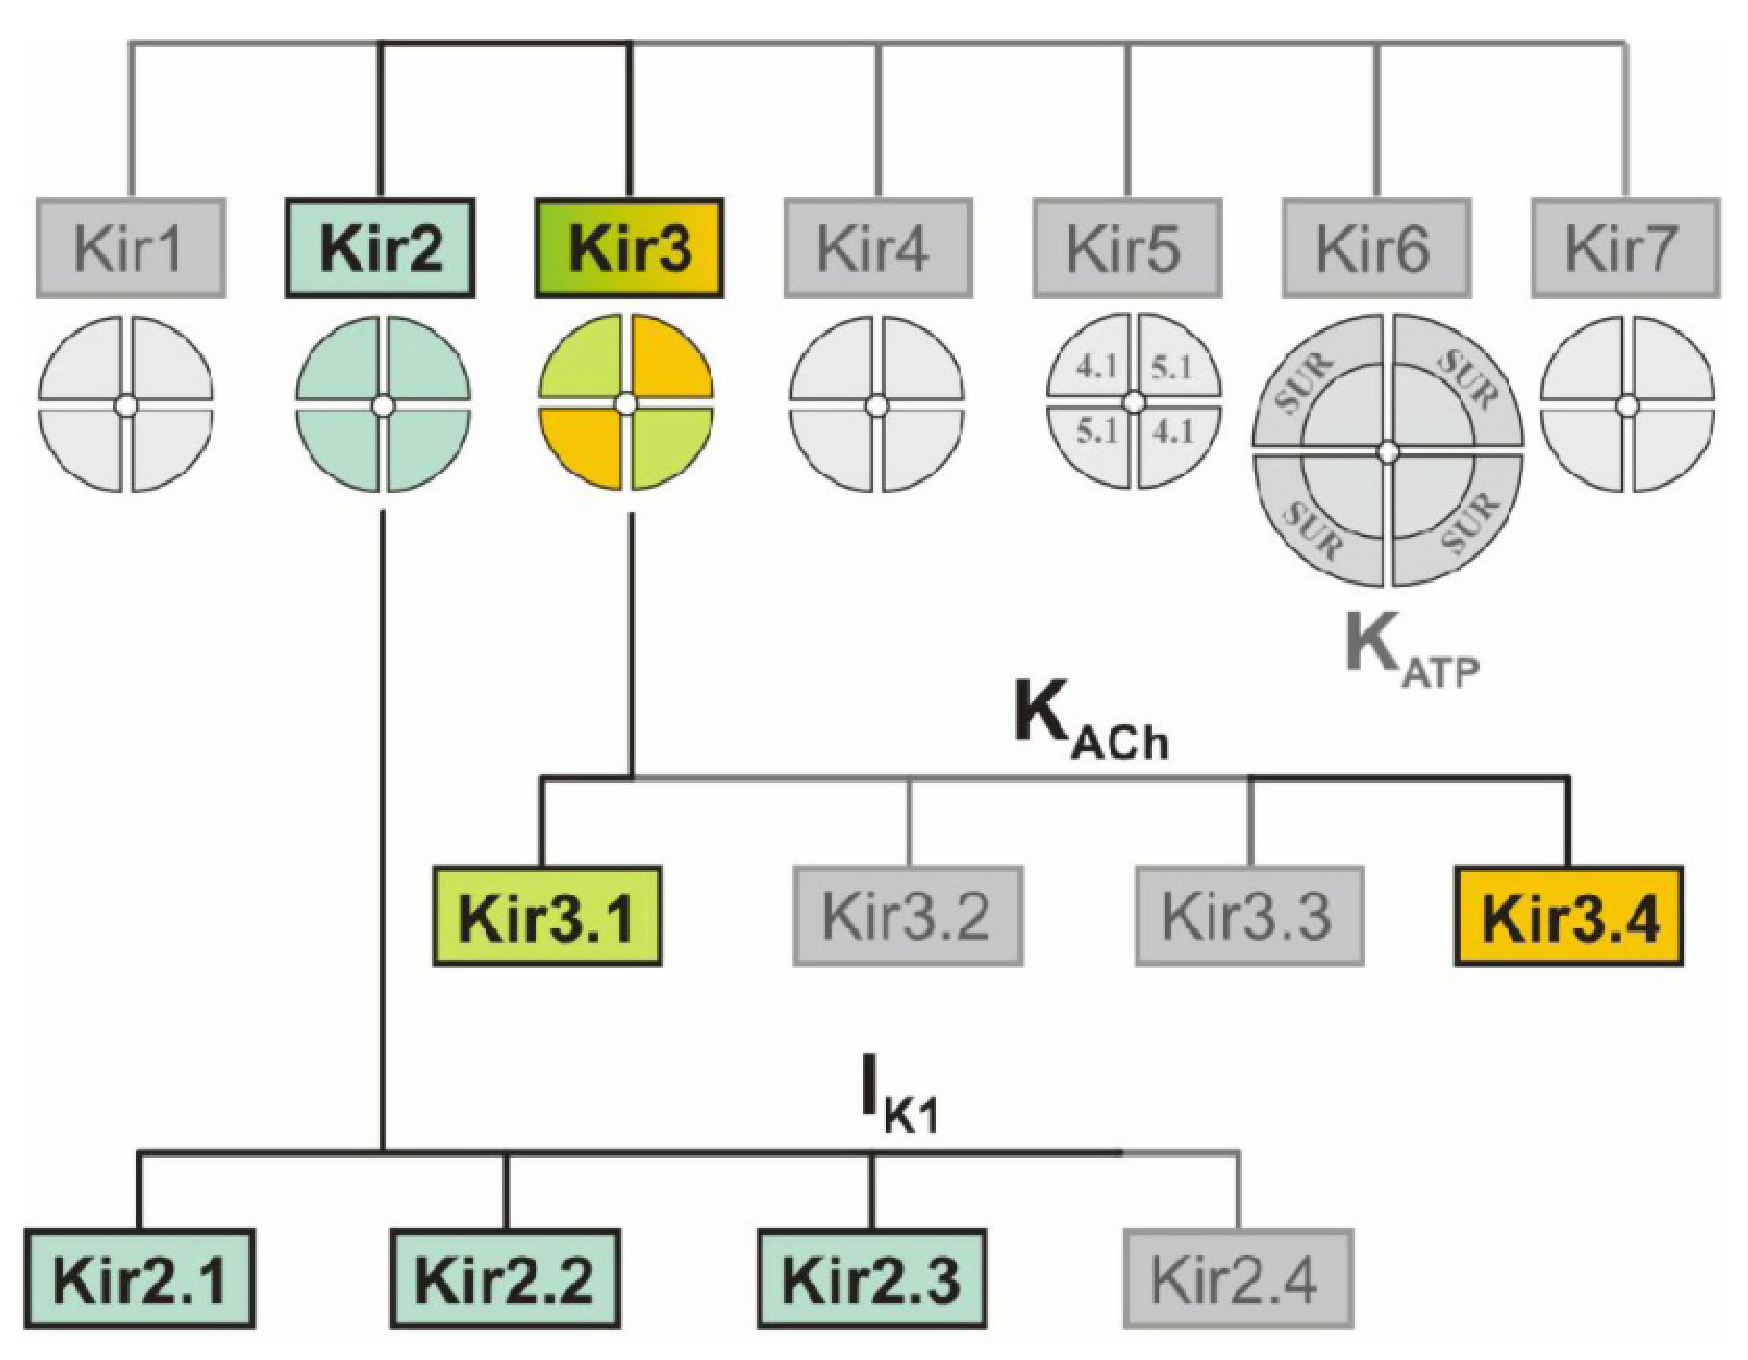
\includegraphics[height=4cm,
    angle=0]{./images/Kir_family.eps}}
\caption{Only Kir2 and Kir3 carry strong rectifying
  current (Fig.\ref{fig:Kir_current}). Heteromeric assemblies of Kir2.1 Kir2.2,
  and Kir2.3 subunits form $I_{K1}$. Heteromeric assemblies of Kir3.1 and Kir3.4
  underlies $I_{\ce{KACh}}$ current}
\label{fig:Kir_family}
\end{figure}


\subsection{-- Classification 1: Kir1.x to Kir7.x}
\label{sec:Kir-classification-genes-based}

{\bf CLASSIFICATION 2} (based on the encoding genes): There are 7 subfamilies
($\Kir$1.x-$\Kir$7.x) each with different members, depending upon the genes that
encoded the channels, found in different cell types \citep{kulbo2005}.
They are also found in multiple prokaryotic isoforms: KirBac1.1-9.

\begin{enumerate}
  \item Kir1
  
  \item Kir2 : Kir2.1, Kir2.2, Kir2.3, and Kir2.4 subunits
  
   $I_{\k 1}$ (Sect.\ref{sec:IK1_current}): is heteromeric assemblies of Kir2.1,
   Kir2.2 and Kir2.3 subunits.
  
  \item Kir3 : Kir3.1, Kir3.2, Kir3.3, and Kir3.4 subunits
  
 They forms G-protein coupled KIR receptors, i.e. $I_{\KAch}$ -
 Sect.\ref{sec:KACh-current} - is heteromeric assembly of Kir3.1 and Kir3.4.
  
  \item Kir4 
  
  \item Kir5
  
  \item Kir6 ($\k_\ATP$)
  
  \item Kir7
\end{enumerate}
In addition to subfamilies shown in Fig.~\ref{fig:Kir_family}, the newly found
ones are:
\begin{enumerate}
\item Kir2.5 : cloned from fish
\item Kir3.5: cloned from {\it Xenopus laevis}
\end{enumerate}



\subsection{-- Classification 2: strong vs. weak}
\label{sec:Kir-classification-signal-strength-based}

Inwardly rectifying potassium channel family members often differ widely in
gating kinetics, as shown in Fig.~\ref{fig:Kir_current}(C). 

{\bf CLASSIFICATION 1}: It is based on the level of rectification
\begin{enumerate}
  \item {\bf weak inwardly rectifier}: Kir4.1 (Sect.\ref{sec:Kir4.1})
      
  \item {\bf strong inwardly rectifier}: Kir2.x and Kir3.x carry strong inwardly
  rectifying current (Sect.\ref{sec:inward-rectifier-strongly}) 
  
They are  Kir2.x and Kir3.x - first found in skeletal muscle, but also found in
glial cells and neurons of CNS.
  
\end{enumerate}

% It can also be classified into two types:
% \begin{enumerate}
%   \item strongly inwardly-rectifying $\Kir$ channel: 
%   
%   \item weakly inwardly-rectifying $\Kir$ channels: 
% \end{enumerate}



% \subsection{Inward rectifier ($\Kir$ \texorpdfstring{$\rightarrow$}{:} $I_{K1}$
% and $I_\KAch$ and $I_\KATP$)}



% Inward-rectifier $I_{K1}$ (or $I_\Kir$) which allows $\K$ influx, and
% help 

\subsection{-- expression levels}

Of the seven main types of Kir channels, at least two (KIR2.x and 3.x) are
present in the MOB. Of the 2.x family, KIR2.1 is highly expressed in
periglomerular cells (Pruss et al., 2005), as well as KIR2.2 (a.k.a.
IRK2/KCNJ12; (Karschin et al., 1996); also KIR2.3 is weakly expressed in the
glomerular layer (Inanobe et al., 2002; Allen Brain Atlas, 2013).

SURx proteins (Sect.\ref{sec:SUR-protein}) are not detected in the MOB (Allen
Brain Atlas, 2013), and therefore the more likely target of the action of
quinacrine are 2.x Kir channels, whose presence in the MOB would be confirmed by
our data.

The presence of KIR3.x channels (G protein-coupled Kir, a.k.a. GIRK, channels)
has been reported in the periglomerular layer of the MOB (Karschin et al.,
1996); the sensitivity of a fraction of the hyperpolarization-activated inward
current to tertiapin, a rather selective blocker of KIR3.1 - 3.4 channels (Jin and
Lu, 1998; Kitamura et al., 2000; Ramu et al., 2008), would confirm this finding.

Quinacrine suppresses a large (46\%) fraction of hyperpolarization-activated
inward current in DA periglomerular neurons. It means 54\% of the this current
comes from Ih-channel (Sect.\ref{sec:Ih-current}).

\subsection{-- kinetics and antagonist}
\label{sec:Kir-kinetics}

\begin{enumerate}
  \item  A voltage-dependent block of the channel pore by polyamines and
  intracellular magnesium is thought to be responsible for the inward
  rectification of these channels (Lopatin et al., 1995) 
  
  \item \ce{Cs^+}-sensitive
  
  \item \ce{Ba^2+} as antagonist
  
  200 $\muM$ $\Ba$ block Kir
  
  \item Quinacrine, which differentially inhibits the Kir channels (KIR2.3 >
  KIR2.1 $\gg$ KIR6.2; (Lopez-Izquierdo et al., 2011)

  \item Muscarine reduce Kir 
   
  \item  inactivation of Kir2.1?
  \begin{itemize}
    \item in a subset of striatal neuron (ENK(+) or ENK/SP(+) neurons) in NAc: 
    inactivation occurs at hyperpolarized potential
    
    \item SP(+)-expressed neurons (in NAc) don't have inactivating KIR; instead
    non-inactivting KIR
    
    \item in striatopallidal neuron in striatum: Kir2.1 has no inactivation
    (Ariano, Levine (2004) - Fig.1(A)), 
    
  \end{itemize}
  
  \item why Kir2.1 does not exhibit inactivation?
  
  The decay of inward current through KIR has been attributed to
  a number of factors:
  \begin{enumerate}
    \item depletion of external $[\K]$ near the channel
    
    \item decrease of $\K$ permeability
    
    \item inhibition by external cations such as $\Na$, \ce{Rb^+}, $\Mg$,
    \ce{Ca^+}, $\Ba$ or $\Ca$
    
 Shieh et al. (2000) suggest it is external $[\K]$; but not other divalent
 cations is the blocker of inactivation, as channel inactivation still present
 with 5mM internal and external EDTA.
 
    \item ML133 is Kir2-specific inhibitor
    
      
    \item the $\Vm$-dependent inactivation is suggested to be indirect
    
    Binding of external $\K$ to the 'inactivation' binding site is
    $\Vm$-independent. 
  \end{enumerate}
   
  \item inactivation Kir2.1:
  
High $[\K]_o$ prevents the Kir channel from inactivation. 

With lower enough $[\K]_o$, internal $[\Mg]_i$ and polyamines induced
time-dependent decay of inward current. The decay was showed to be
Vm-independent in the range -60 mV to -150 mV (Shiel et al. 2000), with order of
potency: spermidine > spermine $\gg$ $\Mg$.

Positive charges, such as $[\Na]_o$, in extracellular media also induces
time-dependent inactivation block (Mermelstein et al., 1998). However, in $\Na$
free condition, the inactivation is still there. 


The inactivation is voltage-dependent, i.e. increasing with hyperpolarization. 
\end{enumerate}

\subsection{-- Classification 3: KATP, K1, GIRK}
\label{sec:Kir-classification-3}

{\bf CLASSIFICATION 3}: Another way to classify the inward-rectifier channels is
using 3 classes:


\begin{enumerate}
  
  \item KATP (K$_\ATP$, ATP-sensitive $\K$ channels):
  $\Kir$6.1, $\Kir$6.2, ATP-dependent ($\Kir$1.1, $\Kir$2.2, $\Kir$4.1)

$I_\KATP$ (Sect.\ref{sec:Kir_KATP}):  only open under pathological condition
(e.g. ischemia) when ATP level is low, i.e. ATP-activated $I_\KATP$.

% $I_\Katp$: another prominent $\Kir$ current found in cardiac cell,
% yet only open under certain pathological condition (e.g. ischemia)
% when ATP level is abnormal.

  \item $\Kir$ ($I_{\k1}$): $\Kir$2.1, $\Kir$2.3, $\Kir$2.4, $\Kir$2.6,
  $\Kir$4.2, $\Kir$5.1, $\Kir$7.1

Denoted as $I_{K1}$ in early papers (Sect.\ref{sec:IK1_current}) as opposed
to $I_{K2}$ used for delayed-rectifier.

  \item GIRK (G-protein activated potassium current -
  Sect.\ref{sec:GIRK}): heteromeric formed by
  $\Kir$3.1, $\Kir$3.2, $\Kir$3.3, $\Kir$3.4 subunits.
  
\end{enumerate}

% There are 3 inward rectifier currents:
% \begin{enumerate}
%   \item  $I_{K1}$ 
%   \item  $I_\KAch$ and 
% \end{enumerate}
% In ventricular myocytes, the more prominent component is $I_{K1}$; while in SA
% node or AV node, the current is receptor-activated denoted as $I_\KAch$. The
% third one, 


\subsection{Comparison with other K+ channels}

\subsection{-- Kir vs. leak K+ current}

Kir conduct substantial current near the resting potential but carry little or
no current at depolarized potentials. However, it is important to know that
inward rectifiers also differ from tandem pore domain potassium channels, which
are largely responsible for "leak" K+ currents (Sect.\ref{sec:leak-K+-current}).

\subsection{-- Kir vs. KcsA}

The activation of Kir channel depolarize the cell membrane, as they are inward
preferably. \textcolor{red}{NOTE}: Even though the animal inward-rectifier $\K$
channels (inwardly rectifying $\K$-selective channels (Kir$X.Y$)) share a common
2TM/P topology (Sect.\ref{sec:2TM/P}) with KcsA (Sect.\ref{sec:KcsA}), they are
otherwise somewhat distantly related with a sequence similarity of only about
15\%. However, further studies between Kir6.2 and KcsA support the use of
KcsA-like models for Kirs (review: \citep{sansom2002}).



\subsection{-- Single channel conductance}

The single channel conductance is about 20pS in cardiac
ventricular cells. The conductances~\citep{Anumonwo2010}: $\sim$20-31 pS for
Kir2.1, $\sim$34-42 pS for Kir2.2, $\sim$10-14 pS for Kir2.3, $\sim$15 pS for
Kir2.4 and $\sim$42 pS for Kir3.1.


\subsection{-- Blockers}

Kir4.1 and Kir2.3 both show fast activation kinetics and slight time-dependent
inactivation, and were blocked by micromolar concentrations of external cesium and
barium.

% The inward $\K$ current ($I_\text{K1}$):
% \begin{enumerate}
% \end{enumerate}

% In Voltage-clamp, the inward rectifier current
% shows a downward deflection, while the outward rectifier current shows an upward
% deflection, Fig.\ref{fig:rectifier_current}. Some inward rectifiers are weak
% inward rectifiers that carry measureable outward $\K$ current. The strong inward
% rectifiers carry very little outward current. They mainly active at voltage
% negative to the reversible potential $E_{\rev,\K}$ where they carry inward
% current (much larger current below the 0nA in Figure above).

\subsection{in glial cells and neurons in CNS}


Kir2.x and Kir3.x are also found in glial cells and neurons of CNS, besides
their presence in cardiac and skeletal cells. Between these two extremes of
strongly inward $\K$ current and weakly inward $\K$ currents, the brain is
particularly well endowed with K channels that have intermediate rectification
properties. Many of these channels are strongly dependent on ligand activation,
often through G proteins or other second messenger systems
(Sect.\ref{sec:Kir_GIRK}).

% In BRAINS:
\begin{enumerate}
  \item IRK (Kir2.0) : best charactered in brain - Sect.\ref{sec:Kir2.0}
  
Neurons in rat NAcc express primarily (Sect.\ref{sec:MSN-K+-currents}).
  
  \item G-protein coupled IRK (Kir3.0): Sect.\ref{sec:Kir3.x}

Kir3.x: Neuronal cells predominantly express GIRK1, GIRK2, and GIRK3 but also
express GIRK4 to a minor extent (Wickman et al., 2000) - Sect.\ref{sec:GIRK}.

\end{enumerate}


\begin{itemize}
  \item Kir activates rapidly; and show little inactivation
  
  \item Kir magnitude depends on the difference between $\Vm$ and $E_\K$, i.e.
  $(\Vm - E_\K)$.

  \item The gating of KIR is strongly dependent on $[\K]_e$. The reason is that:
  KIR is blocked by intracellular $\Mg$ and polyamines, at potential positive to
  $E_\K$.
    
  \item Kir is blocked in a time- and voltage-dependent manner by low
  concentrations of extracellular Barium (0.01 - 0.1 mM).
  
  \item Kir is blocked in a solely voltage-dependent manner by higher
  concentration of Cesium (2 - 10 mM) and TEA (> 20 mM)
\end{itemize}



\subsection{in cardiac and skeletal}
\label{sec:Kir-cardiac-skeletal}

Kir2.1, Kir2.2, and Kir2.3 are the three isoform that form the tetrameric ion
channel $I_\Kir$ in cardiac and skeletal cells.

$K_\ATP$ is also found in cardiac cells (Sect.\ref{sec:Kir_KATP}).


\subsection{weak inwardly rectifier}
\label{sec:inward-rectifier-weakly}

Note that these channels are not perfect inward rectifiers, as they can pass
some significant outward current at positive potential, e.g. in the voltage
range up to about +30 mV above resting potential. 

However, they are different from outward rectifiers
(Sect.\ref{sec:K_outward-rectifier}) which are considered as more "typical"
potassium channels preferentially and carry outward (rather than inward)
potassium currents at depolarized membrane potentials.

MEMBERS:
\begin{enumerate}
  \item Kir4.1 - Sect.\ref{sec:Kir4.1}
  
  \item K-ATP - Sect.\ref{sec:Kir_KATP}
\end{enumerate}

\subsection{-- Kir4.1}
\label{sec:Kir4.1}

Kir4.1 channels are weakly inwardly rectifying potassium channels
(Sect.\ref{sec:inward-rectifier-weakly}) that critically regulate extracellular
K+ levels and are expressed in the CNS primarily by astrocytes
(Sect.\ref{sec:astrocyte-perivascular-endfeet}).

One of the major physiological roles of potassium channels in glial cells is to
promote 'potassium spatial buffering' in the central nervous system, a process
necessary to maintain an optimal potassium concentration in the extracellular
environment. This process requires the precise distribution of potassium
channels accumulated at high density in discrete subdomains of glial cell
membranes (Connors, Kofuji, 2004).
\begin{enumerate}
  \item  Kir4.1 is associated with the dystrophin-glycoprotein complex (DGC) in
  mouse brain and cultured cortical astrocytes, through PDZ domain-mediated
  interaction with $\alpha$-syntrophin.
 
Kir4.1 can bind directly to $\alpha$-syntrophin, requiring the presence of the
last three amino acids of the channel (SNV), a consensus PDZ domain-binding motif

 Kir4.1 failed to associate with the DGC in brains from $\alpha$-syntrophin
 knockout mice.
 
  \item AQP4 (waver aquaporin 4) needs agrin to segregate to perivascular
  astrocytic endfeet, and the process is also mediated by
  agrin binding to $\alpha$-dystroglycan (a member of dystrophin-dystroglycan
  complex - DDC). This couples AQP to $\alpha$1-syntrophin - a member of DC.
  
This  explains the co-localization of Kir4.1 and AQP4
\end{enumerate}


As the inward current is not dominant, the channels carry measurable outward
K+ currents (about 0.5 nA) at voltages positive to the K+ reversal potential
$E_{\rev,\K}$. %, and no inward current

In the hippocampus, Kir4.1 shows only moderate expression compared to other
brain regions (Nwaobi et al., 2014). 

\subsection{-- ATP-sensitive Potassium channel (KATP)}
\label{sec:Kir_KATP}

Similar to Kir4.1, $\KATP$ channels display only weak rectification
(Sect.\ref{sec:inward-rectifier-weakly}) and allow substantial outward current
to flow at positive potentials.

ATP-sensitive potassium channels ($\Katp$) were first found in cardiac cells by
Noma ~\citep{Noma1983}. $\Katp$ are expressed in numerous tissue types including
skeletal muscle, brain, kidney, purheart, pancreatic b-cells, and smooth muscle.
The channels are typically found in sarcolemmal (sarc$\KATP$)
\citep{inagaki1995}, mitochondrial (mito$\KATP$) \citep{inoue1991}, or nucleus
(nuc$\KATP$) \citep{quesada2002}.
\begin{itemize}

  \item $\Katp$ have been found to be modulated by pH, fatty acids, NO, SH-redox
  state, various nucleotides, G-proteins and various ligands (adenosine,
  acetylcholine, benzopyrans, cyanoguanidines, etc.).
  
  \item  The receptors are A1 purinergic receptor~\citep{sorota1998}.  The
  suggested pathway is that (1) adenosine stimulates A2 receptors, which
  activates adenylyl cyclase; (2) the resulting
increase  intracellular cAMP stimulates protein kinase A, which, probably
through a phosphorylation step, opens KATP channels \citep{kleppisch1995}.
\end{itemize}


In smooth muscle, an ATP-sensitive $\K$ channel activated by Adenosine $K_\ADO$
was found \citep{kleppisch1995}. The functional role in vascular smooth muscle
has also been studied \citep{brayden2002}.

\subsection{----- : Kir6.1, Kir6.2 and SUR subunits}
\label{sec:Kir_KATP_Kir6.1-6.2-SUR}
\label{sec:SUR-protein}

ATP-sensitive $\K$ channels is composed of $\Kir$6.x subunits ($\Kir$6.1 and
$\Kir$6.2) and sulfonylurea receptors (SUR) subunits. 

SUR is the protein that regulate the sensitivity to pharmacologic agents and
ATP. 

$\Kir$6.x subunits has 2 transmembrane domain, and SUR subunits have 3
transmembrane domains.
\begin{enumerate}
  \item Sarc$\KATP$ has 4 $\Kir$ subunits and 4 SUR subunits, giving them
  totally 8 subunits (octamer). The true ratio varies upone tissue type.
  \item Mito$\KATP$'s components is less known.
  \item Nuc$\KATP$ was recently confirmed from isolated patches of nuclear
  membranes, with kinetics similar to Sarc$\KATP$.
\end{enumerate}

\textcolor{red}{$\Katp$ are inhibited by physiologic levels of ATP}
and, as ATP falls, channel open probability increases (although the degree of
ATP reduction needed would rarely be seen under physiologic conditions.
When mitochondria function declines, which produce less ATP for the cell, to
conserve energy, sarc$\KATP$ open, reducing the duration of AP while
nuc$\KATP$-mediated $\Ca$ concentration changes within the nucleus.
Experimental studies showed $\Katp$ openers exert profound {\bf cardioprotective
pharmacology} effect in numerous mammalian species~\citep{Grover2000}.

\subsection{----- : Kir1.1 (ROMK), Kir2.2, Kir4.1}
\label{sec:Kir_KATP_Kir2.1-2.2}

There are other ATP-dependent $\K$ channels:
\begin{enumerate}
  \item $\Kir$1.1  (aka ROMK (renal outer medullary potassium channel)) is
  encoded by KCNJ1 gene.
  
  \item $\Kir$2.2 is encoded by KCNJ12 gene. This is one of the multiple
  inwardly rectifying channels that contribute to the cardiac inward rectifier
  current IK1.
  
  \item $\Kir$4.1 is encoded by KCNJ10 gene. This channel is found in glial
  cells in brain.
\end{enumerate}

In cardiac cells, we have $\Kir$1.2.

\url{http://en.wikipedia.org/wiki/ATP-sensitive_potassium_channel}.

\subsection{strong inwardly rectifier: Kir2.x, Kir3.x}
\label{sec:inward-rectifier-strongly}
\label{sec:Kir-strong}

Among the different subfamilies, Fig.~\ref{fig:Kir_family}, only two subfamilies
Kir2 and Kir3 (Sect.\ref{sec:Kir-classification-genes-based}) fit to the
definition of {\it strong inwwardly rectifying current} and are classically
found in skeletal and cardiac muscle, with different level of
expression~\citep{Anumonwo2010}.

An inward rectifier carry $\K$ ions inwardly through the cell membrane much more
efficient than outwardly (at hyperpolarized potential); even though the $\K$
concentration gradient is outward (Sect.\ref{sec:concentration-K+-ion}), as the
channel pore is blocked in a voltage-dependent manner.

There are two types of strong inwardly rectifier K+ channel: one  formed
by (homogenous or heterogenous) Kir2.x subunits (Sect.\ref{sec:Kir2.x}) or
by Kir3.x subunits (Sect.\ref{sec:Kir3.x}).

These (strong) inward rectifier $\K$ channels has a high conductance at negative
voltages (i.e. carry inward current about -6.2 nA near the K+ reversal
potential, as shown in Fig.\ref{fig:rectifier_current}) which allows cells to
maintain a stable resting potential. Such conductance reduces with membrane
depolarization. Very little current flows through the
channels at potential positive to -40 mV.

NOTE: The high conductance at negative  voltage allows cell to maintain a
stable resting potential; yet the greatly reduced outward conductance during
membrane depolarization avoids short-circuiting the generating of action
potential.

% The channels carry very little outward current at all, and are mainly active
% at voltages negative to the K+ reversal potential to carry the inward current
% (about -6.2 nA)

\subsection{-- Kir2.x (IRK: Kir2.1, Kir2.3)}
\label{sec:Kir2.x}
\label{sec:Kir2.0}

Kir2.x is a class of strong inwardly rectifier
(Sect.\ref{sec:inward-rectifier-strongly}), which has inward current at
negative membrane potential, and is a main driver for resting membrane
potential. Kir2.1 is very similar to the cardiac inward rectifier K+ current
(IK1) - Sect.\ref{sec:IK1_current}.

At negative membrane potential, the voltage-dependent blockade of
outward currents by the intracellular polyamines spermine and spermidine
enables the inward current to flow.
Upon membrane depolarization (up to around -60mV), the inward currents is
strongly reduced, due to the blocking of
intracellular Mg2+ and spermine (SPM) in physiological conditions
\citep{huang2016}
\begin{itemize}
  \item  a bundle-crossing region is responsible for the flux-coupling blocking
  phenomena of SPM 
  
  I176 to A184 residues constituting the bundle-crossing region might also be
  involved in the blocking effect of SPM.
  
  However, 10 $\mu$M SPM can not fully block the outward currents even at strong
  depolarization.
  
  \item it has been reported that 0.5-1 mM Mg2+, and 1-20 $\mu$M SPM at
  physiological concentrations both have qualitatively similar flow- and
  voltage-dependent blocks of the Kir2.1 channel.
  
  S165, a residue in the transmembrane domain marking the
  external end of the central cavity in the Kir2.1 channel, is reportedly crucial to intracellular
  Mg2+ but not SPM block
  
  \item Only Kir2.3 are sensitive to Muscarinic receptor activation -
  Sect.\ref{sec:M-current}
  
  Kir2.3 is found on postsynaptic side of excitatory synapses.
  
\end{itemize}

\textcolor{red}{MECHANISM:} 
Early and incorrect studies beliefed that intracellular $\Mg$ can block
Kir2, which compete with $\K$ for entry into the channel's pore
~\citep{Guo2002}. 

Nowadays, essential properties of rectification can be explained by
\begin{itemize}
\item potent and strongly $V_m$-dependent block of Kir2 channels by
  intracellular organic cations called polyamines which can be found
  in many cell types at low milimolar
  range~\citep{Cohen1998}. However, most polyamines are bound to RNA,
  DNA, and ATP, leaving only a few can cause rectification in Kir
  channels~\citep{Yan2005}.

  \textcolor{red}{Among different polyamines (spermine, spermidine and
    putrescine), spermine is the most potent inducer of rectification,
    then to spermidine, putrescine}, and lowest is $\Mg$.
\end{itemize}

Residues critical for inward rectification are D172, a ``rectification
controller'', E224, E299.
\begin{itemize}
\item In Kir2, D172 in charges of ``steep'' (highly voltage
  dependent), and E224, E299 are ``shallow'' (less voltage dependent)
  of the rectification. 
\end{itemize}

In human, Kir2.1 is the dominant isoform underlying ventricular $I_{K1}$, and
lower role in atrial $I_{K1}$~\citep{Gaborit2007}. The gene that encode Kir2.1
is KCNJ2. The mutation at this gene can cause loss- or gain-of-function
\citep{lopatin2001}. When the membrane depolarize, the channel pass an {\it
outward current} to help end the AP. However, when the membrane potential is
hyperpolarized (below -85 mV), the channel passes a large {\it inward} $\K$
current. Inward rectifier channels are found in many cell types (cardiac,
kidney, neurons, etc.).

In guinea pig, Kir2.4 is found localized to neuronal cells only. So, the current
$I_{K1}$ from cardiac myocytes is supposed to be the contribution from these
channels Kir2.1-2.3.
    
NOTE: Kir2.5 : cloned from fish


\textcolor{red}{REGULATORS}: The channel is blocked by
\begin{enumerate}
  \item TEA (internal) - Sect.\ref{sec:TEA}
  \item Cs and $\Ba$.
\end{enumerate}


Flecainide does not modify Kir2.2 or Kir2.3, yet preferentially
increased the outward IKir2.1 generated at physiological potentials.
So, flecainide increase $I_{K1}$ at ventricular myocyte, but not in
atrial myocytes. It does so by increasing $P_o$ of Kir2.1 channels,
not modifying unitary current amplitude. The location where Flecainide
bind to Kir2.1 is Cys311~\citep{Caballero2010}.


\url{http://en.wikipedia.org/wiki/Inward-rectifier_potassium_ion_channel}
\url{http://www.ncbi.nlm.nih.gov/pubmed/14977398}

%\subsection{----- \texorpdfstring{K1 channel: $I_{K1}$}{K1 channel}}
\subsection{----- K1 channel (cardiac)}
\label{sec:IK1_current}
%\subsection{Inward-rectifier $I_{K1}$ current (ventricular myocyte)}

The inward-rectifier $I_{K1}$ is the channel found in cardiac myocyte  and is
supposed to be the result of multiple inward-rectification $\Kir$ channels, i.e.
Kir2.1-2.3 (Sect.\ref{sec:Kir2.x}).


\subsection{-- Kir3.x (GIRK): G-protein coupled IRK}
\label{sec:Kir_GIRK}
\label{sec:Kir3.x}
\label{sec:GIRK}
%\subsection{G-protein coupled IRK (Kir3.0)}
\label{sec:Kir3.0}

%   There are several subfamilies of inward rectifier: $K_\ATP$, GIRK/$\Kir$
%   (G-protein coupled inward-rectifier), etc.

G protein-coupled inwardly-rectifying $\K$ channels (GIRKs) is a type of G
protein-coupled receptor (GPCRs)-activated potassium channel with string inward
rectification (Sect.\ref{sec:inward-rectifier-strongly}).

The GPCRs that can activate GIRK channels are \citep{yamada1998}
\begin{enumerate}
  \item serotonergic (5-HT1A), 
  
  \item GABAergic receptor type B (GABA-B) - Sect.\ref{sec:GABAB-receptor} 
  
  \item muscarinic (m2), 
  
  \item adenosine (A1), 
  
  \item opioid ($\mu$, $\delta$, and $\kappa$),
  
  \item adrenergic ($\alpha$2), and 
  
  \item dopaminergic (D2) receptors
\end{enumerate}

Upon activation, such  GPCRs release activated G$_{\beta\gamma}$-subunits from
inactive G$_{\alpha\beta\gamma}$. G$_{\beta\gamma}$-subunits then interact with
the GIRK channels to gate the channel.

\textcolor{red}{As an inward current, GIRK is important in maintenance of the
resting membrane potential, regulation of action potential duration, and
receptor-dependent modulation of cellular excitability.}
When activated, GIRK channels typically decrease the firing rate of
atrial myocytes and neuronal cells.

There are 4 subtypes: GIRK1-3 channels (encoded by KCNJ3, KCNJ6, KCNJ9 genes,
respectively) are found in central nervous system, GIRK4 channels (KCNJ5 gene)
is found primarily in the heart.
\begin{enumerate}
  \item GIRK4 = Kir3.4   (known as CIR)
  \item GIRK3 = Kir3.3
  \item GIRK2 = Kir3.2 - Sect.\ref{sec:GIRK2.x}
  \item GIRK1 = Kir3.1

  \item Kir3.5: cloned from {\it Xenopus laevis}
\end{enumerate}




\subsection{------ GIRK1/GIRK4 heteromer (Kir3.1/Kir3.4): $I_\KACh$ current (MK,
muscarinic potassium channel, acetylcholine-activated potassium channel KAch, M current)}
\label{sec:KACh-current}
\label{sec:IKAch_current}
\label{sec:MK-channel}
\label{sec:M-current}

M-current refers to the current that is sensitive to the activation of
Muscarinic receptors (Sect.\ref{sec:muscarinic-acetylcholine-receptor}).

M-current are potassium current, and is reduced by 
\begin{verbatim}
ACh --> M1-receptor --> Galpha,beta-gamma  --> PLC-beta

PIP2 level increase --> DAG  + IP3

IP3 --> release [Ca2+] via IP3R

DAG --[require Ca2+]--> PKC 
    PKC modulate Kv7/M-current via PKC phosphorylation
    PKC modulate Kir current
\end{verbatim}

\begin{enumerate}
  \item M1-type receptor reduce Kir2.3 current - Sect.\ref{sec:Kir2.x}
  
  \item slow voltage-gated M-channel (KCNQ) - Sect.ref{sec:KCNQ}
\end{enumerate}


M current is a type of slow, noninactivating voltage-gated outward potassium
current (Sect.\ref{sec:Kchannel_Vm-dependent}) first discovered in bullfrog
sympathetic ganglion cells. The name ``M'' is named after the antagonis
muscarine (when ACh acting muscarine receptors) and several peptide
neurotransmitter. 

and these are called

\begin{itemize}

  \item \textcolor{red}{atrial tissue} (SA node and AV node):  muscarinic
  potassium channels ($I_\KACh$ or MK-current, acetylcholine-activated potassium
  channel) .

Kir3.2, Kir3.3 were not found in atrial cells, leaving Kir3.1 (GIRK1) and Kir3.4
(GIRK4) the only candidate for cardiac $I_\KACh$ (Sect.\ref{sec:KACh-current}).

In atrium and nodel cells, $K_\ACh$ current helps decreasing the heart rate, and
was suggested to be anovel target in treatment of atrial fibrillation (AF)
\citep{walsh2010}. Upon the activation of {\bf m}uscarinic
acetylcholine-activated receptor (MAChR), it increases the outward flux via the
M-current, thus suppressing the net inward flux \citep{adams1982}.

  
  \item \textcolor{red}{neurons}: MK channel (M-current) encoded by 2-subunits
  of GIRK1 and 2-subunits of GIRK4

The channel is found in vertebrate central neurons and sympathetic cells.
The channel is regulated by neurotransmitter and second messenger, e.g.
muscarinic receptors (Sect.\ref{sec:muscarinic-acetylcholine-receptor}).
M channel is PIP2-regulated ion channel (Sect.\ref{sec:PIP2}).


\textcolor{red}{The inward rectifier in cardiac cells doesn't respond to
  muscarine}\citep{sakmann1983aas}.

    \item  mixed complex of KCNQ2/3 and KCNQ3/4 (Sect.\ref{sec:KCNQ}): show a
    relatively hyperpolarized activation threshold ($\approx$ -60 mV).

They contribute to M CURRENTS in sympathetic neurons and the central nervous
system, and are inhibited by muscarinic receptor activation and are associated
with familial epilepsy - Sect.\ref{sec:M-current}.
     
KCNQ1 subunits gain prominent expression in the ear and heart and are associated
with inherited deafness and arrhythmia; MiRP2-KCNQ1 complexes have been shown to
allow for the passage of K+ ions at rest in experimental cells.

     
\end{itemize}
In some cases, an ``M'' current is part of a ``delayed rectifier''
(Sect.\ref{sec:delayed-rectifier}). The current activates at membrane potential
closed to the resting one or at hyperpolarized potentials.

   
% This type of G protein-coupled
% inward-rectifying current $I_\KACh$ is supposed to be the result of two types of
% $\K$ channels: GIRK1 and GIRK4.

At first $I_\KAch$ was thought to be encoded by GIRK1 gene only (G-protein
activated inward rectifying K1 channel $I_{K1}$)\citep{costa2005}. Nowaday, we
know that it is a heteromultimer encoded by two distinct genes: GIRK1 (2
subunits, Kir3.1) and GIRK4 (2 subunits, Kir3.4) \citep{krapivinsky1994}; with
the receptor for the agonist is muscarinic M2 cholonergic receptor~\citep{soejima1984}.

KAch current is more prominent in atrial tissue, i.e. SA node and AV node.
As no other GIRK genes was found in the heart, heteromeric assemblies of Kir3.1
and Kir3.4 underlies $I_{\ce{KACh}}$ current (Sect.\ref{sec:Kir3.x})


M channel is unique because it is open at rest and even more likely to be open
during depolarization. M-channels are the reason for slow depolarizations
produced by neurotransmitter.
\begin{enumerate}
  \item initial depolarization increase $P_o$ of M-channel
  \item opening M-channels generate an outward potassium current, which 
  counteract the inward $\Na$ current. 
  
  \item Overall result: full action potential is   prevented.
\end{enumerate}
The M-channel is important in raising the threshold for firing an action
potential. 

\url{http://en.wikipedia.org/wiki/M_current}



\subsection{------ GIRK2.x (Kir3.2)}
\label{sec:GIRK2.x}






%\subsection{$I_{BK_\ca}$}


\subsection{TWIK}

Sect.\ref{sec:TWIK-1-channel}.

\subsection{Inward-rectifying Kv11.x channel}

Kv channels also display inward rectification properties. There are three of
them: Kv11.1 (hERG in human, gene KCNH1 - Sect.\ref{sec:HERG_channel}), Kv11.2 and
Kv11.3.

\subsection{$I_\kCa$}

\subsection{$I_\kNa$}

\subsection{$I_\kFFA$}
% \subsection[\texorpdfstring{$\Kir$ channels KIR}{Kir
% PIP2-gated channels}]{Inward-rectifier \texorpdfstring{$\Kir$ channels}{Kir
% channels}:
% Ligand-activated ($I_\Kir$, $I_\KAch$ ($I_{K1}$), $I_\KAdo$ $I_\kATP$,
% $I_{K,min}$, $I_{BK_\ca}$, $I_\kCa$, $I_\kNa$ and $I_\kFFA$)} 


\subsection{$I_{K,min}: 1TM$}
\label{sec:IK_min-current}

The singletransmembrane domain, voltage-dependent minK channel.



\subsection{Proton-activated $\K$ channels: KcsA}
\label{sec:KcsA}

KcsA had been the only available structure for potassium channel until 2006.
A good review of \ce{K+} channels before this landmark
was~\citep{armstrong1998vic}.

This canonical $\K$ channel  is a tetramer formed by 4 symmetrical subunits,
each with 2TM/P (Sect.\ref{sec:2TM/P}); which was first found in KcsA channel
(Sect.\ref{sec:KcsA}).
The bacterial (prokaryotic) channel KcsA (PDB entry 1BL8) - found in {\it
Streptomyces lividans} is also the one whose crystal structure of a \ce{K+}
channel was first found \citep{doyle1998}. Even a subunit is 2TM/P, its sequence
in the pore structure (from residual 23 to 119) is very similar to that of
eukaryotic K+ channels (Shaker genes - Sect.\ref{sec:Shaker-gene}) so it is
widely used to study properties of K+ channels.

Based on the X-ray crystal structure of KcsA, the insight into the mechanism of
selectivity and permeation process has been revealed. 
\begin{enumerate}
  \item resolution data at 3.2 \AA
  
  \item narrow selectivity filter: 12 \AA long
  
  \item a large cavity: 10 \AA diameter (near the middle of the membrane)
  
A K+ ion move through the internal pore and cavity;
\begin{itemize}
  \item from inside: the K+ ion can move to outside and still remain mostly
hydrated.
  \item the narrow selectivity filter separating the cavity with extracellular
  solution, makes K+ harder to move inside, i.e. as it has to shed its hydrating
  waters to enter.
  
\begin{mdframed}

NOTE: When an ion enters the selectivity filter, it evidently dehydrates (nearly
completely). To compensate for the energetic cost of dehydration, the carbonyl
oxygen atoms must take the place of the water oxygen atoms, come in very close
contact with the ion, and act like surrogate water.

Also, the two $\K$ ions at opposite ends of the selectivity filter, at about
7.5\AA distance (about the distance between $\K$ ions in a 4mM KCl solution) and
resulting in mutual repulsion (hence their positions nearly at opposite ends).
When a new $\K$ ion comes into the pore, the attractive force between a K1 ion
and the selectivity filter becomes perfectly balanced by the repulsive force
between ions, and this is what allows conduction to occur.

\end{mdframed}

\end{itemize}

Electrostatic calculations show that when an ion is moved along a narrow pore
through a membrane, it must cross an energy barrier that is maximum at the
membrane center. The inner pore and cavity lower electrostatic barriers without
creating deep energy wells. The structural and chemical design of this part of
the pore ensure a low resistance pathway from the cytoplasm to the selectivity
filter, facilitating a high (outward) throughput.
  
  \item two $\K$ ions on the filter, and is 7.5 \AA apart
  
  \item permeability $\K$ $\approx \ce{Rb^+}$ > $\ce{Cs^+}$ (with radius: K+
  1.33 \AA; Rb+ 1.48 \AA; Cs+ 1.69 \AA); very very small permeability for the
  smallest alkali metal ions such as $\Na$ or \ce{Li^+} (with smaller radius:
  Na+ 0.95 \AA; Li+ 0.60 \AA; these ions have more electron dense than that of
  K+, Rb+ and Cs+); i.e.
  permeability of $\K$ is 10,000x more that of $\Na$ (a
  \textcolor{red}{throughput rate approaching the diffusion limit - about $10^8$
  ions per second})
  
  \item ion can permeate in both direction; and ionic mixture result in {\it
  anomalous conductance behavior}.
  
  \item the pore can be blocked by tetraethylammonium
(TEA) ions from both sides.
\end{enumerate}
This configuration promotes ion conduction by exploiting electrostatic
repulsive forces to overcome attractive forces between K+ ions and the
selectivity filter.



\begin{itemize}
  \item  KcsA : found in bacteria, proton-activated and open at acidic pH (i.e.
  lowering of pH).
  
  \item ???
\end{itemize}

\textcolor{red}{The gating requires the presence of $\Mg$ ions.} 

\label{sec:KcsA-channel-blockers}
{\bf Blockers}:   KcsA channel can be blocked internally (TEA and also the
inactivation domain located at the N-terminus of some Kv channel) or externally
(tetraethylammonium (TEA) and various peptide toxins).


\section{Kv family (Vm-gated Kv{\it X.Y}): 6TM/P}
\label{sec:Kchannel_Vm-dependent}

The $V_m$-dependent $\K$ channel ($\Kv$, KvX.Y) is a homo-tetramer formed by 4
$\alpha$-subunits of the same type (6TM/P - Sect.\ref{sec:6TM/P}), i.e. no
subunits from different families can form a functioning Kv channel.
In mammals, these channels are widely expressed in brain, muscle and heart where
they control complex waveforms of electrical activity.

Our understanding of this family of potassium channels mainly come from
Drosophila genes (Sect.\ref{sec:Kv-Drosophila}) and some from non-Drosophila
genes (Sect.\ref{sec:Kv-non-Drosophila}). They are indeed outward current
(Sect.\ref{sec:K_outward-rectifier}), and the notation for mammalian potassium
channels is Kv$X.Y$, with $X$ has 4 values 1 to 4, mapping to the four
equivalent genes in Drosophila (Shaker, Shab, Shaw, and Shal -
Sect.\ref{sec:Kv-Drosophila}).


\subsection{1.A. Drosophila potassium genes (Kv1, Kv2, Kv3, Kv4)}
\label{sec:Kv-Drosophila}

There are 4 related subfamilies of Drosophila potassium channel genes Shaker,
Shaw, Shal and Shab (Butler et al., 1989).
\begin{enumerate}
  \item Shaker - Sect.\ref{sec:Kv1-channels}
  \item Shaw - Sect.\ref{sec:Kv2-channels}
  \item Shal - Sect.\ref{sec:Kv3-channels}
  \item Shab - Sect.\ref{sec:Kv4-channels}
\end{enumerate}


\subsection{- Kv1 subfamily (Shaker gene): Regulator of conductance of K+ (RCK
channels)}
\label{sec:Kv1-channels}
\label{sec:Shaker-gene}

Kv1 class is aka {\bf Shaker-related channels}, due to the fact that the  gene
({\it Sh} gene) that encoded the channel (found in fruit fly) when mutated cause
the fly's leg to shake.  Shaker-related potassium channels (or {\bf regulator of
conductance of K+} RCK channel) are A-type K+ channels
(Sect.\ref{sec:A-type-K+current}) from mammals whose gene similar to the one
first clone from Drosophila Shaker mutants belong to Kv1 subfamily.

\begin{itemize}
  \item found mainly in muscle cell (Sect.\ref{sec:A-type-K+current-myocyte})
  
  \item expressed in rat brain (Stuhmer et al. 1989), e.g. striatum

\begin{enumerate}
  
  \item In neurons of the medial trapezoid body, heteromers of Kv1.1, Kv1.2, and
  Kv1.6 subunits are important regulators of repetitive spiking (Dodson et al.
  2002).
  
  \item Striatum: Kv1.2 (KAs - Sect.\ref{sec:KAs-current}) 
\end{enumerate}
  %beside Raw proteins
  %(Sect.\ref{sec:Raw-K+-channel})
\end{itemize}

Depending on the genes that encode the Kv1 channel, they can have different
names, e.g. Kv1.1 (KCNA1 gene), Kv1.2 (KCNA2), Kv1.3 (KCNA3), Kv1.4, Kv1.5
(KCNA5), Kv1.6 (KCNA6), Kv1.7 (KCNA7), Kv1.8 (KCNA10).

Kv1 raises AP firing threshold; responsible for the repolarization of the
membrane potential.

\textcolor{red}{\bf Antagonist}:
\begin{enumerate}
  \item $\alpha$-DTX (Sect.\ref{sec:alpha-DTX}) blocks all 3 types
  Kv1.1, Kv1.2, and Kv1.6
 
Kv1.1, Kv1.2, and Kv1.6 channels can form homomeric or heteromeric ion channels.
In heterologous expression systems, Coetzee et al. 1999 showed that (1) the
slowly inactivating current is sensitive to 4-aminopyridine (4-AP) at micromolar
concentrations and to $\alpha$-dendrotoxin ($\alpha$-DTX), and (2) the recovery
from inactivation is slow (Shen, Surmeier (2004); Day, Surmeier (2008)).

  \item other Kv1 family toxins that lacks a high affinity for Kv1.2 subunit:
  r-agitoxin-2, dendrotoxin-K, and r-margatoxin.

  \item {\bf DTX-K (100nM)}: only block channels containing Kv1.1 subunits
  (Robertson et al. 1996; Wang et al. 1999b).
  
  \item {\bf r-margatoxin (MgTX; 30 nM):} only block channels containing Kv1.3
  subunits
  
  \item {\bf AgTX (10 nM)}: a high-affinity blocker of Kv1.1, Kv1.3, and Kv1.6,
  but not Kv1.2 (Garcia et al. 1994)
\end{enumerate}


\subsection{- Kv2 subfamily (Shab gene)}
\label{sec:Kv2-channels}
\label{sec:Shab-gene}

Voltage-gated K+ channels from mammals whose gene similar to the one first clone
from Drosophila Shab mutants belong to Kv2 subfamily.
The function of the expressed proteins can be changed by the modulating of
Kv5-Kv10 genes (Sect.\ref{sec:Kv-non-Drosophila}). Most of the delayed rectifier
current (Sect.\ref{sec:delayed-rectifier}) are the products of the {\it Shab}
gene \citep{tsunoda1995}.

Kv2 class is {\bf Shab-related channels}. Depending  on the genes that encode
Kv2 channels, they can have different names, e.g. Kv2.1 (KCNB1 gene), Kv2.2
(KCNB2).
   
Kv2 influences AP repolarization and hyperpolarizes the inter-AP membrane
potential during high frequency firing.
Kv2.1/2.2 channels are more slowly deactivating than Kv3.1/3.2 (Hwang et al.,
1992; Kirsch et al., 1993) - Sect.\ref{sec:Kv3-channels}.
This prolonged deactivation of these channels at negative membrane potentials
should increase the relative refractory period, effectively slowing discharge
rates. \textcolor{red}{By regulating the coexpression of these Kv3 and Kv2
family channels, neurons may tune their discharge patterns effectively}.

\begin{mdframed}
The names Shaker, Shaw, Shab, and Shal are  based on the genes encoding
potassium-selective channels that were found in fruit fly {\it Drosophila}; and
each has been shown to have human homology.
These channels has pore-forming $\alpha$ subunits that associate with different
types of $\beta$ subunits. The fourth TM  domain has positively charged
residues that can act as voltage sensor.

\end{mdframed}

\subsection{- Kv3 subfamily (Shaw gene): Raw channel (TEA and 4-AP sensitive)}
\label{sec:Kv3-channels}
\label{sec:Shaw-gene}
\label{sec:Raw-K+-channel}

Kv3 class of K+ channel is found prominently in \textcolor{red}{brain, and
retinal ganglion cells} (Sect.\ref{sec:Kv3-channels}). The Shaw-related rat
potassium channel family is dubbed {\bf Raw}.

Unlike other voltage-gated K+ channels, Raw K+ channels exhibited intense
rectification due to a voltage-dependent block by internal $\Mg$.
\begin{itemize}
  \item expressed in rat brain (Rettig et al. 1992) 
\end{itemize}

Kv3 subfamily channels regulate firing frequency of auditory and fast-spiking
GABAergic interneurons, accelerates AP repolarization. They are sensitive to TEA
respectively for half-blocking).

Kv3 channels have the rapid and steeply voltage-dependent activation and
deactivation kinetics of which are well-suited for generating narrow action
potentials and short refractory period, with up to 1 kHz.

The potassium channel subunit KV3.1b is localized to somatic and axonal
membranes of specific populations of CNS neurons. 

\subsection{---- Kv3.1, Kv3.2}
\label{sec:Kv3.1}
\label{sec:Kv3.2}

The striatum contains a subpopulation of fast-firing GABA-ergic interneurons
characterized by the presence of immunoreactivity for the calcium-binding
protein, parvalbumin.

In the dorsolateral striatum, only parvalbumin mRNA-positive neurons expressed
the mRNA encoding the potassium channel Kv3.1

Kv3.1-Kv3.2 channels play critical roles in the generation of fast-spiking
properties in cortical GABAergic interneurons (Rudy, 2006).
Kv3.1/3.2 channels are unique in their ability to deactivate within 1 msec at
260 mV (Vega-Saenz de Miera et al., 1994; Robertson, 1997).
Several studies have concluded that these channels underlie a 'fastspiking'
pattern found primarily in GABAergic interneurons (Du et al., 1996; Massengill
et al., 1997; Martina et al., 1998; L. Wang et al., 1998). E.g.: blocking a
rapidly deactivating Kv3-like K1 current reduces the ability of interneurons to
discharge at high frequencies

\subsection{---- Kv3.3}
\label{sec:Kv3.3}

Kv3.3 increases the spontaneous firing rate via cooperation with resurgent
sodium currents (Akemann, 2006).




\subsection{- Kv4 subfamily (Shal gene)}
\label{sec:Kv4-channels}
\label{sec:Shal-gene}

Kv4 class is {\bf Shal-related channels}. This is the most complex class of
$V_m$-gated ion channels from structural and functional standpoints.
Shal-gene encodes some forms of A-current (Sect.\ref{sec:A-type-K+current}) in
neurons.
%%not right -->, i.e. A-type K+ current is encoded by Kv4 subunits.

A-type K1 channels with Kv4-like properties are prominent in
(Sect.\ref{sec:A-type-K+current-neuron})

\begin{enumerate}

  \item in {\bf neostriatal cholinergic neurons} are
  attributable to K+ channels containing Kv4.2 a subunits (Song et al., 1998).

NOTE: single-cell reverse transcription-PCR (scRT-PCR) and patch-clamp studies
(Sect.\ref{sec:scRT-PCR}).

  \item somatodendritic regions of other central and peripheral neurons . 

NOTE: Immunocytochemical studies (Sheng et al., 1992; Maletic-Savatic et al., 1995;
Alonso and Widmer, 1997); and reverse transcription-PCR (scRT-PCR) and
patch-clamp studies (Johns et al., 1997; Dryer et al., 1998; Martina et al.,
1998) - Sect.\ref{sec:scRT-PCR}.

  \item neurons in the basal ganglia, e.g. spiny projection neurons (SPN).
  
\end{enumerate}
   
\subsection{1.B. Non-Drosophila genes (Kv5, Kv6, Kv8, Kv9, Kv10)}
\label{sec:Kv-non-Drosophila}


Kv5, Kv6, Kv8 and Kv9 are newly cloned electrically-silent $\alpha$-subunits
which don't possess any functional activity; but appear to form heteromeric
channels with Kv2 subunits. So, they modulate Shab channel activity
(Sect.\ref{sec:Kv2-channels}) \citep{salinas1997}.
\begin{enumerate}
   \item Kv5 (KCNF)
   \item Kv6 (KCNG)
   \item Kv8 
   \item Kv9 (KCNS)
   \item Kv10 class is voltage-gated non-inactivating delayed rectifier $\K$
   channel: Kv10.1 (KCNH1), Kv10.2 (KCNH5)
\end{enumerate}


\section{Kv family - section 2}
\label{sec:Kv_channel}

In the previous section Sect.\ref{sec:Kchannel_Vm-dependent}, we describe a form
of classifying Kv-family channels, mainly based on study from Drosophila with
Kv1-Kv4 genes. Those from Kv5-Kv10 are not found in Drosophila.


In this section, we provide a different approach of how Kv-family channels are
named, based on the kinetics of the channels. 
They can be
\begin{enumerate}
  \item outward rectifier - Sect.\ref{sec:K_outward-rectifier}
\end{enumerate}
In general, Kv family are outward
potassium currents which are closed at the resting potential, but activated at
different rates by depolarization, i.e. outward rectifiers.

\subsection{Outward rectifiers (KDR + KA)}
\label{sec:K_outward-rectifier}

The early detected potassium channels, e.g. the one used in Hodgkin-Huxley
model (Sect.\ref{sec:cek+-conductance}), is an outward delayed rectifier which
plays an important role in repolarizing the membrane potential after an AP.
This is, however, not the unique outward $\K$ channel in different cell types. 

Depending upon the genes that express the protein, outward rectifier $\K$
currents can be classified into
\begin{enumerate}
  \item transient outward currents (KA, I$_A$, Ito, 'A'-current, IKt) -
  Sect.\ref{sec:K_outward-rectifier}: and may be thought of as "outwardly
  rectifying."

The outward currents with both transient (KAf) and sustained (KAs) components
(KAf - Sect.\ref{sec:KAf-current}; KAs - Sect.\ref{sec:KAs-current}).
There are different mechanisms leading to channel inactivation.
  
  \item (outward) delayed rectifier currents (KDR, Kdr, IKv3.1, non-'A' current)
  - Sect.\ref{sec:delayed-rectifier} - the sustained component (i.e. with slow
  recovery from inactivation).
  
  \item non-inactivating $\K$ current - KRP (Sect.\ref{sec:KRP})
\end{enumerate}

\textcolor{red}{However, there are other potassium channels also display outward
rectifying properties}
\begin{enumerate}
  \item TOK1 - Sect.\ref{sec:TOK-1_current}
\end{enumerate}

KAf, KAs and non-inactivating $\K$ currents are depolarization-activated outward
current; while KDR is repolarization-activated outward current. In opposite
direction to outward current is the inward rectifier $\K$ current -
Sect.\ref{sec:inward-rectifier-Kir}.


\begin{mdframed}
Using patch-clamp analysis on intact axons of Jellyfish {\it Aglantha digitale},
K+-selective channels that form the basis of outward current can be divided into
4 different classes, based on their range of kinetics.
All 4 classes have the same conductance characteristics (Robert W. Meech,
Chapter 20, Evolution of the First Nervous System).

% \begin{enumerate}
% 
%   \item rapidly-inactivating A-type - Sect.\ref{sec:A-type-K+current}
% 
%   \item non-inactivating delayed rectifier
% \end{enumerate}
%https://play.google.com/store/books/details?id=vEYGCAAAQBAJ&rdid=book-vEYGCAAAQBAJ&rdot=1&source=gbs_vpt_read

\end{mdframed}
% These channels to carry transient (Sect.\ref{sec:Kv_Ito}) or sustained
% (Sect.\ref{sec:Kv_DR}) potassium outward currents. 

% There are two outward rectifiers $\K$ currents:
% \begin{itemize}
%   \item KA (A-type current): transient outward rectifier -
%   Sect.\ref{sec:A-type-K+current}
%   \item Kdr: (outward)  delayed rectifier - Sect.\ref{sec:delayed-rectifier}
% \end{itemize}

\subsection{A. A-type potassium channel (fast/rapid activating, rapidly
inactivating) (K$_A$ channels): 4-AP sensitive}
\label{sec:A-type-K+current}
\label{sec:Ito_channel}

The membranes of most excitable cells contain a distinct set of potassium
channels that can rapidly open and close following depolarization, giving rise
to the transient outward $\K$ current, $I_A$ (A-type current) (Rogawski, 1985).

The name {\bf A-type current} derives from the typical profile of
\begin{enumerate}
  \item rapid activation at subthreshold voltages; followed by fast inactivation
  of the current (becomes inactivated at above approximately -40mV
(Sect.\ref{sec:A-type-K+current-Connor-Stevens-1971})).

   \item the time constants are intermediate between $g_\Na$ and $g_K$ of
   delayed rectifier ($I_K$ in Hodgkin-Huxley's work, i.e. contribute to
   repolarization) and thus predominate during the middle and latter part of the
   interspike interval.
\end{enumerate}
This biophysical diversity is matched by the  molecular heterogeneity.
Genes with A-type properties are found in several sub-families of Kv channels
Kv1 (Shaker-like), Kv3 (Shaw-like), and Kv4 (Shal-like) -
Sect.\ref{sec:Kv-Drosophila}. At least 6 genes code for K+ channel subunits that
form A-type K+ current: \textcolor{red}{Kv1.4; Kv3.4; Kv4.1; Kv4.2; Kv4.3; and
erg3} (review: Tkatch, Surmeier, 2000).

Aldrich and co-workers (Solc et al., 1987) first discovered 2 different forms of
A-type current (Sect.\ref{sec:A-type-K+current-Drosophila})
\begin{enumerate}
  \item $A_1$ current
  
  \item $A_2$ current (Shaker-gene) 
\end{enumerate}

% At least six genes code for K+ channel subunits that form A-type channels in
% heterologous expression systems: Kv1.4, Kv3.4, Kv4.1-3, and erg3 (Stuhmer et
% al., 1989; Baldwin et al., 1991; Pak et al., 1991; Roberds and Tamkun, 1991;
% Schroter et al., 1991; Serodio et al., 1996; Shi et al., 1997).

Because of this diversity in properties, A-type K+ channels serves different
functions depending upon the cell types
(Sect.\ref{sec:A-type-K+current-function}) Also, co-expression of accessory
subunits with certain Kv $\alpha$-subunits confers rapid inactivation to
otherwise noninactivating (Sect.\ref{sec:MK-channel}) or moderately inactivating
delayed rectifier channels.
The auxiliary channel subunits can transform non-inactivating, delayed rectifier
K+ channels into inactivating, A-type channels (Rettig et al., 1994; Heinemann
et al., 1996).


\begin{mdframed}

{\bf A-type currents} were first observed in {\it Onchidium} neurons
(inverterbrate, molluscan neurons) by Hagiwara, Kusano and Sato; and later its
kinetics was characterized in {\it Nudibranch} molluscan neurons by Connor and
Stevens (Hagiwara et al., 1961; Connor and Stevens, 1971) with a characteristic
(as we just mentioned) {\bf transient (i.e. early outward current), rapidly
inactivating} K+ current.

The existence of $I_A$ in primitive metazoan organisms, such as the sea
pansy Renilla, suggests A-current arose early in evolution, possibly even before
the appearance of Vm-gated $\Na$ channels.

\end{mdframed}

In vertebrate, rapidly inactivating, A-type K+ currents have been found in a
wide variety of mammalian neurons (Rudy, 1988); yet they have a wide biophysical
properties and only those with Kv4 family subunits appear to have properties
similar to those originally described in invertebrates - that is, an ability to
open at subthreshold membrane potentials and to recover quickly from
inactivation (Serodio et al., 1994) - Sect.\ref{sec:A-type-Kv4-like}.



\subsection{** functions}
\label{sec:A-type-K+current-function}

A-type K+ channels serves different functions depending upon the cell types 
(Sect.\ref{sec:A-type-K+current-function})

\begin{enumerate}
  \item {\bf neurons}: $I_A$ determine the interval between consecutive spikes
  during repetitive spikings - Sect.\ref{sec:A-type-K+current-neuron}
  
  \item {\bf cardiac myocyte}: $I_\to$ control the initial repolarization of the
  myocardium. - Sect.\ref{sec:A-type-K+current-myocyte}

  \item {\bf smooth muscle cell} - Sect.\ref{sec:A-type-K+current-smoothmuscle}
\end{enumerate}

\textcolor{red}{A-type K+ current plays prominent role in spike repolarization
(Storm 1987), controlling spike frequency, and integration of synaptic input}
(the level of A-type K+ activation can produce different shunting effect).
Like the majority of ion-channels, A-type channels generally contain additional
regulatory proteins
% Storm, J.F., Action potential repolarization and a fast
% after-hyperpolarization in rat hippocampal pyramidal cells, J. Physiol.
% (Lond.), 385 (1987) 733-759
 
\begin{enumerate}  
  \item  $\beta$-subunits that induced fast-inactivating properties and
  fine-tune their properties, including trafficking, location and abundance,
  sensitivity to stimulation, pharmacology and gating
  (Sect.\ref{sec:Kv-ancillary-subunits}).
  
  NOTE: The $\alpha$-subunit is non-inactivating voltage-dependent function.
  
  \item KChIP auxiliary proteins - Sect.\ref{sec:KChIP}
\end{enumerate}

So, A-type currents are voltage-gated (Sect.\ref{sec:Kchannel_Vm-dependent})
potassium (Kv) currents that undergo {\it transient (rapid) activation} (at
subthreshold range of $\Vm$). The kinetics of inactivation can be splitted into 2
components: {\bf rapid inactivation} or {\bf slower inactivation} (during
depolarization pulses of duration). Depending on the organs, we have two
different notations:

\begin{itemize}

  \item $I_A$ current in neurons: there are 2 components: KAf (faster
  inactivation), and KAs (slower inactivation) -
  Sect.\ref{sec:A-type-K+current-neuron}.
  
  \item $\Ito$ current in atrial and ventricular myocytes: Itof (faster
  inactivation), Itos (slower
  inactivation) Sect.\ref{sec:A-type-K+current-myocyte}:
\end{itemize}

Neher [ref], and Thompson [ref]. They are found in both cardiac
(Sect.\ref{sec:A-type-K+current-myocyte}) and neuronal cells
(Sect.\ref{sec:A-type-K+current-neuron}); and also are identified and
characterized in vascular, genitourinary, and gastrointestinal smooth muscle
cells (Sect.\ref{sec:A-type-K+current-smoothmuscle}).
In human, the channel is formed by Kv4.x subunits (Sect.\ref{sec:Kv4-channels}).


The apparent multiplicity of roles played by the A-current may be a reflection
of different subtypes of channel with distinctive gating properties, i.e.

\begin{enumerate}

  \item by activating transiently (the transition of $m$ activation from 0 to
  1): it can filter out or limit the depolarizing synaptic inputs.
  
  \item by inactivating slowly (the transition of $h$ inactivation gate
  from 1 to 0 is slow): it slowly permit the membrane to depolarise towards the
  spike threshold. 
\end{enumerate}

\begin{enumerate}
  
  \item some A-type currents (A-like current): open at subthreshold, inactivate
  quickly and recover quickly from inactivation (e.g. those found in
  invertebrates).
  
NOTE: only channels composed of Kv4 family subunits appear to have properties
similar to those originally described in invertebrates-that is, an ability to
open at subthreshold membrane potentials and to recover quickly from
inactivation (Serodio et al., 1994) - Sect.\ref{sec:Kv4-channels}.

  \item  some A-type (or 'A-like') currents inactivate rapidly but recover from
inactivation very slowly, taking seconds at hyperpolarized membrane potentials. 


  \item some A-type currents activate only at suprathreshold membrane
  potentials, rather than at subthreshold potentials, predisposing them to a
  role in spike repolarization. 

  \item The molecular picture is further complicated by the ability of auxiliary
  channel subunits to transform non-inactivating, delayed rectifier K1 channels
  into inactivating, A-type channels (Rettig et al., 1994; Heinemann et al., 1996).

  \item the  role for IA in delaying the time to first firing and in integration
  (in the mathematical sense) of synaptic inputs have been proposed for hippocampal
pyramidal cells (Storm, 1988), for thalamic relay cells (McCormick, 1991), and
for striatal spiny projection neurons (Nisenbaum et al., 1994).
 
\end{enumerate}


\subsection{** distribution}

There is now direct evidence that $I_A$ channels are present on dendrites, as
well as on the somata and axons of some mammalian neurons (Sheng et al., 1994).



% A-type was discovered when experiments by Connor and Stevens on some encoding
% membranes, e.g. gastropod neurone soma, showed an additional outward K channel
% type, known as transient (rapidly) inactivating A-type (''A'') current $I_A$
% ($K_A$ channels), which is encoded by {\it Shal} gene
% (Sect.\ref{sec:Shal-gene}). 

\subsection{A.1. Drosophila}
\label{sec:A-type-K+current-Drosophila}

Aldrich and co-workers (Solc et al., 1987) have described two types of fast
transient A-channels in {\it Drosophila}, which they term A1 and A2, in two
different cell types; both have different conductance, voltage-dependence and gating kinetics.

The two are distinguished primarily by their voltage-dependence, with about 30mV
shift in voltage-dependence of HVA current (Surmeier, 1989).
\begin{itemize}
  \item  The A1 channel (found in myotube) is activated at {\it relatively
  depolarized potentials} and has rapid inactivation kinetics -
  Sect.\ref{sec:A1-K+-current}.

The expression of this membrane protein is either blocked or altered by
mutations of the Shaker locus (Sect.\ref{sec:Shaker-gene}). 

The A1 current is the principal repolarizing current following a spike in pupal
flight muscle and axons. This is mapped to KAs current found in mammalian neuron
(Sect.\ref{sec:KAs-current}).
  
  \item The A2 channel protein (found in neuron) is activated at less
  depolarized potentials, has slower inactivation kinetics than the A1 current
  and is unaffected by the Shaker mutation - Sect.\ref{sec:A2-K+-current}.
  
  Due to the low threshold activation, A2 channel may be more important in
  controlling repetitive firing in {\it Drosophila} neurons than in spike
  repolarization. This is mapped to KAf current found in mammalian neuron
(Sect.\ref{sec:KAf-current}).
\end{itemize}
%Solc, C.K., Zagotta, W.N. and Aldrich, R.W., Single-channel and genetic
% analyses reveal two distinct A-type potassium channels in Drosophila, Science 236 (1987) 1094-1098.

At single-channel level:
\begin{enumerate}
  \item A1 channel: 12-16 pS; with complete inactivation with 500-ms prepulse to
  -20mV
  
  \item A2 channel: 5-8 pS; with complete inactivation with 500-ms prepulse to
  -80mV
\end{enumerate}
In mammalian sensory neuron, the single A-current conductance are different,
with 20pS; and inactivation time constant in the range 30ms to 100ms (see more
details in Sect.\ref{sec:A-type-K+current-neuron},
Sect.\ref{sec:A-type-K+current-myocyte} and
Sect.\ref{sec:A-type-K+current-smoothmuscle}.


At macroscopic level, A1 channels are faster and more voltage-dependent
macroscopic inactivation rate, a larger steady-state component, and a less
negative steady-state inactivation cullre than the A2 neuronal currents.

\subsection{--- (myotube) A1 current: 4-AP miliMolar (2-5mM) sensitive}
\label{sec:A1-K+-current}

A1 current is one A-type K+ current found in Drosophila
(Sect.\ref{sec:A-type-K+current-Drosophila}). The time courses of both
macroscopic activation and inactivation of the myotube A1 current were voltage
dependent. The current turned on slowly at low voltages.
As the voltage was increased, it turned on faster and developed a larger and
more rapidly inactivating component that decayed to a steady-state value.

These myotube currents are similar in both voltage dependence and kinetics to
the A currents recorded in adult muscle (Salkoff, Wyman, 1980) at a similar
temperature (20$^\circ$ to 23$^\circ$C) and were similarly blocked by 5 mM
external 4-AP.

The myotube current showed no reduction in amplitude after a prepulse to -50 mV,
a prepulse voltage that almost completely inactivated the neuronal current. This
amount of sustained current is also voltage-dependent. This suggests that the
inactivation is non-completed in this type of channel.

\subsection{--- (neuronal) A2 current: 4-AP miliMolar (2-5mM) sensitive}
\label{sec:A2-K+-current}

A2 current is one A-type K+ current found in Drosophila
(Sect.\ref{sec:A-type-K+current-Drosophila}). The neuronal A current (i.e. A2
channel) behaved differently from A1 current.

The macroscopic activation rate was voltage-dependent only at the lowest
voltages, and the macroscopic inactivation rate was largely independent of
voltage over the entire range studied. The neuronal current inactivated
completely with a double-exponential time course that was slower than the rate
of decay seen in myotube A current.


\subsection{A.2. mammalian neurons: A-type Kv4-like channels}
\label{sec:A-type-K+current-neuron}
\label{sec:K+current_4-AP-sensitive}
%\subsection{--- neurons (KAf, KAs): Kv4}

In many neurons, A-type channels (Sect.\ref{sec:A-type-K+current}) are
unavailable at resting membrane potentials due to pronounced steady-state
inactivation (this is in contrast to that in myocyte -
Sect.\ref{sec:A-type-K+current-myocyte}).

A-type channels become available in these cells during afterhyperpolarizations
following action potentials, when the membrane potential becomes sufficiently
negative to remove inactivation \citep{cai2007}.
The opening of A-type channels during the decay of the afterhyperpolarization
tend to delay depolarization. Thus, the opening of the channels can slow down
the return of the membrane potential toward the value of readiness for a new AP,
which eventually prolong the interspike interval (prolong the period between
action potentials, i.e. {\bf regulate firing frequency}).

% In many neurons, A-type channels are usually silent at $V_\rest$; yet
% transiently activate during the decay of the after-hyperpolarization phase of
% AP, delaying depolarizations .
A-type currents determines the interval between two consecutive AP during
repetitive firings. That explains the low frequency firing pattern of neuron at
low depolarization found in certain crab leg axon.

The 4-AP sensitive K+ currents is composed of two components, which
are differentiated based on their kinetics of recovery from inactivation and
their sensitivities to 4-AP (Surmeier et al.
1991, 1994): transient, inactivating KAf (Sect.\ref{sec:KAf-current}) and
slowly, (non-inactivating or inactivating) KAs (Sect.\ref{sec:KAs-current}).

\begin{enumerate}
  \item Granule cell:
  
It's suggested that Kv4 subunits are the major components of $I_A$ in central
nervous system (CNS) \citep{serodio1998}.
Expression of dominant-negative mutant Kv4.2 (Kv4.2dn) in cultured cell
eliminate A-type current, suggested that A-type channels is formed by
Kv4.2 subunits.

An inactivating,  A-type-like channel can be formed when a channel of Kv1 family
coexpressed with ancillary Kv $\beta_1$ subunit \citep{shibata2000}.
  
  \item Purkinje fiber:

The presence of $K_A$ current in Purkinje fiber was given by Kv1.4, Kv3.4 and
Kv4 subunits  \citep{hounsgaard1988}.

  \item Hippocampus:
  
  The Kv1.4-containing A-type $\K$ channels are found in similar regions
  to Kv1.1. channels \citep{cooper1998}. 

  Kv1.4-containing A-type currents are particularly targeted to axons and
  possibly terminals, suggesting a pre-synaptic role in synaptic transmission.

\end{enumerate}
  

\begin{figure}[hbt]
  \centerline{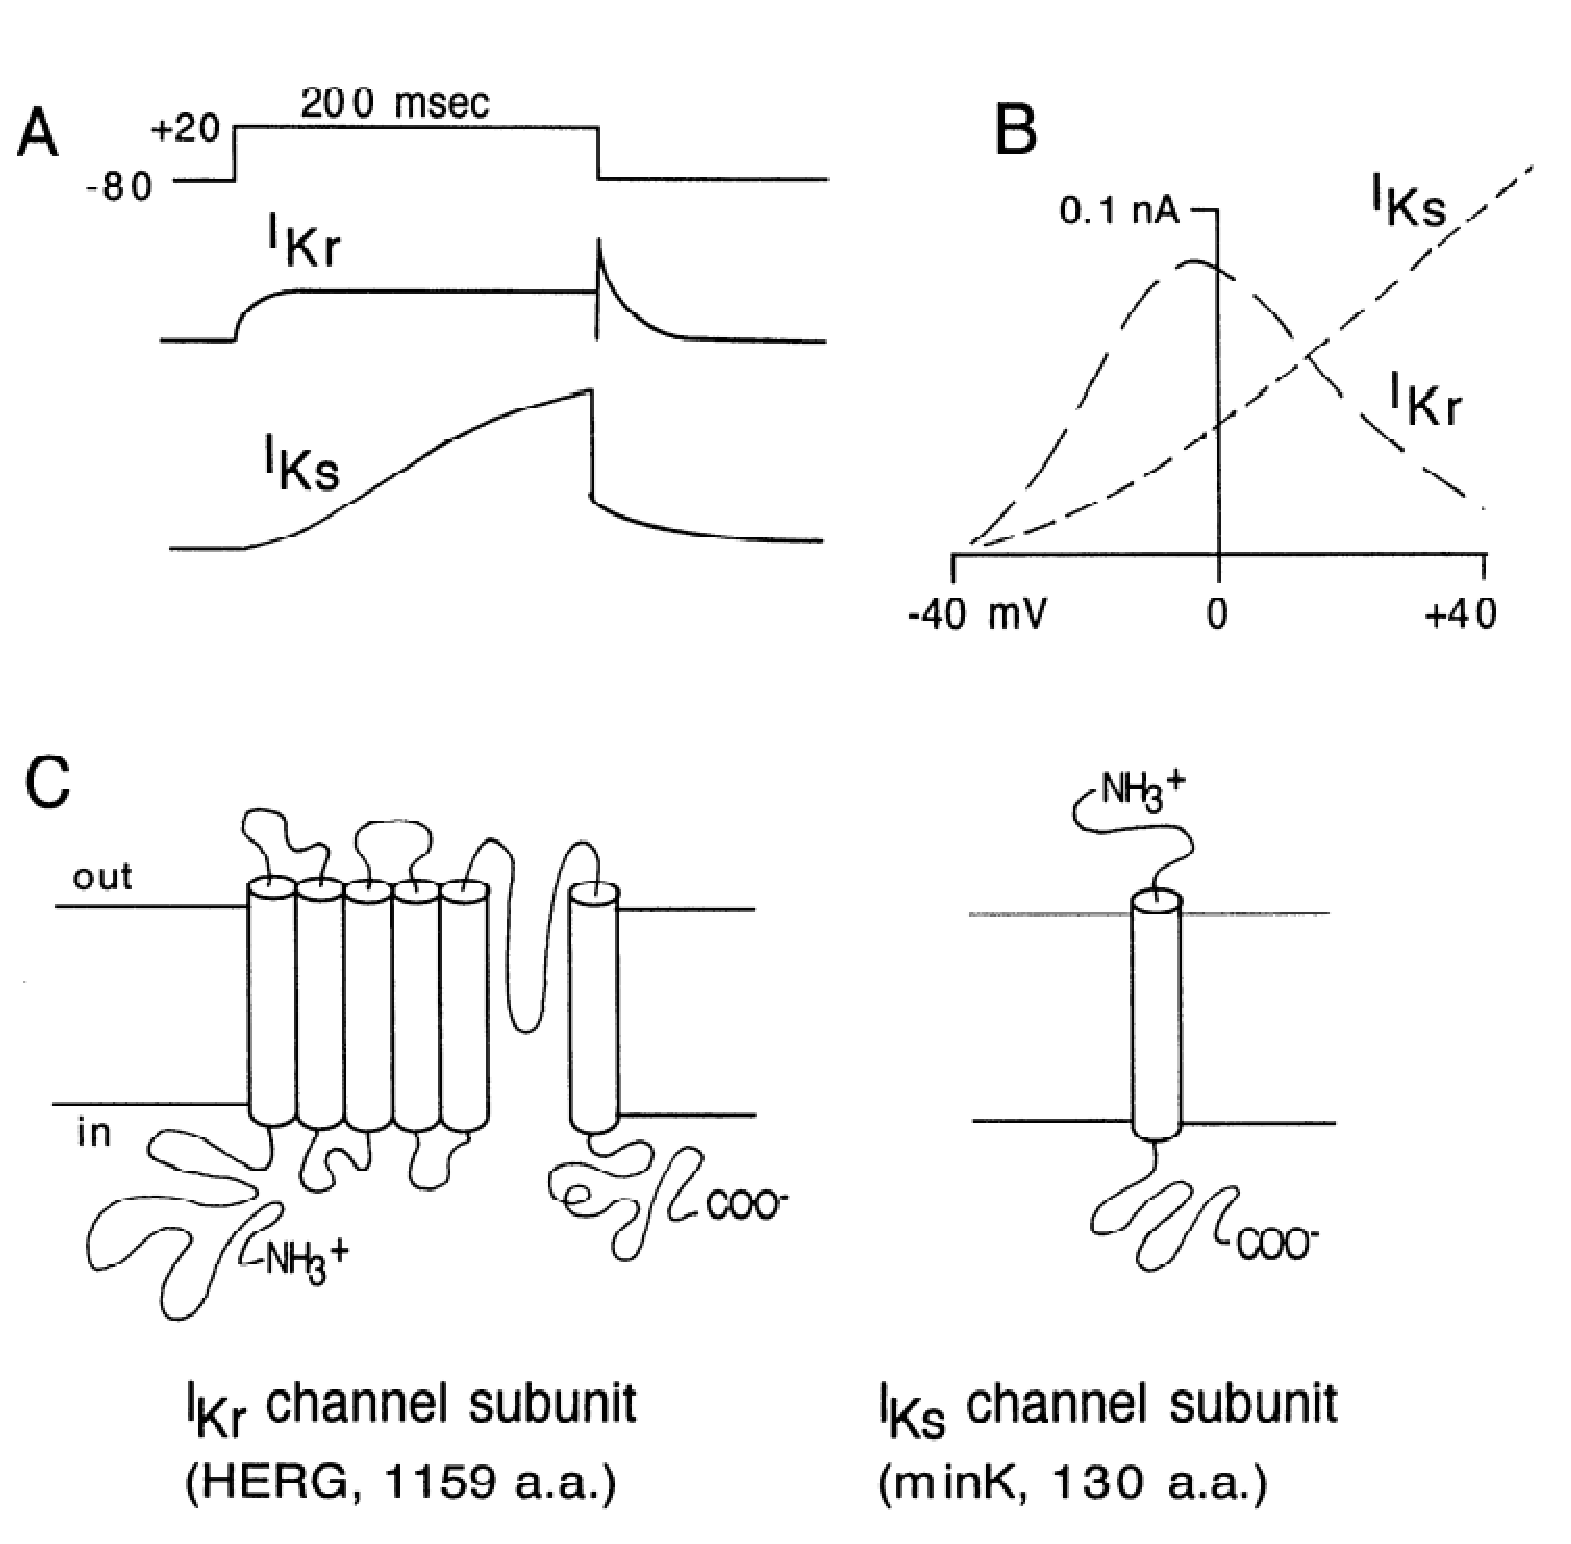
\includegraphics[height=5cm,
    angle=0]{./images/IKr_IKs_currents.eps}}
  \caption{2 components of delayed rectifier $\K$ current \citep{sanguinetti1997}}
\label{fig:Kcurrent_IKs_IKr}
\end{figure}


\subsection{------  4-AP (miliMolar range) sensitive K+ current: KAt (KAf): 
Kv4.2}
\label{sec:K+current_4-AP-sensitive-KAt}
\label{sec:KAf-current}
\label{sec:A-type-Kv4-like}

KAf is the first (and fast) component of the transient 4-AP sensitive A-type K+
current (Sect.\ref{sec:A-type-K+current}) in neurons.
% The time constant is fast and was voltage-independent, i.e. $\tau = 40$ms (at
% potential test +5mV to +35 mV).
In nerve cells, the transient outward $\K$ current $I_A$  ($\KA$ channels) is
fast but brief acting, i.e. open within a few milliseconds after membrane
depolarization at or above spike threshold ($\approx$ -45 mV) with time constant
$\tau_h \approx 10$ (ms), but then rapidly close (inactivate), within 20-100ms
(typically 50ms).

In striatal neurons, KAf is
\begin{enumerate}
  \item blocked by 4-AP at relatively high concentration with IC50 = 2 mM
  
  \item blocked by dendrotoxin (DTX) with IC50 = 1 $\muM$ (Surmeier et al.,
  1988, 1991)
\end{enumerate}


A-type K+ channels with Kv4-like properties (Sect.\ref{sec:Kv4-channels}) are
prominent in the somatodendritic membrane of many mammalian brain neurons,
including neurons in the basal ganglia. In other words, A-type K+ channels in
neurons are the same as the K+ channel encoded by {\it Shal} gene in Drosophila
(Sect.\ref{sec:Shal-gene}).  A discussion for general A-type K+ channels is
given in Sect.\ref{sec:A-type-K+current}.

Kv4.2 channel (Sect.\ref{sec:Kv4-channels}) has been shown to be a major
contributor to A-type potassium current in striatal neurons (Tkatch et al.,
2000) and has kinetics similar to the classic KAf current (Surmeier et al.,
1989).

Fig.\ref{fig:4-AP_Kcurrent} shows the 4-AP-sensitive K+ current
(Sect.\ref{sec:4-AP}) in spinal cord astrocyte.
In striatal neurons (Sect.\ref{sec:medium_spiny_neurons}), 10 mM 4-AP can
completely block the transient component (IC50 is 125 $\mu$M 4-AP); while
reducing the persistent component by 40\%. So, the persistent component is
called 4-AP resistance, persistent K+ current (KRP - Sect.\ref{sec:KRP}).
 
% They are voltage-dependent, $\Ca$-independent K+ outward current, with 2
% components:
% 
% \begin{enumerate}
%   \item fast A-type current (Sect.\ref{sec:A-type-K+current}): KAf, KAt
%   
%   \item 4-AP resistance persistent A-type current (KRP): 
% \end{enumerate}


\begin{figure}[hbt]
  \centerline{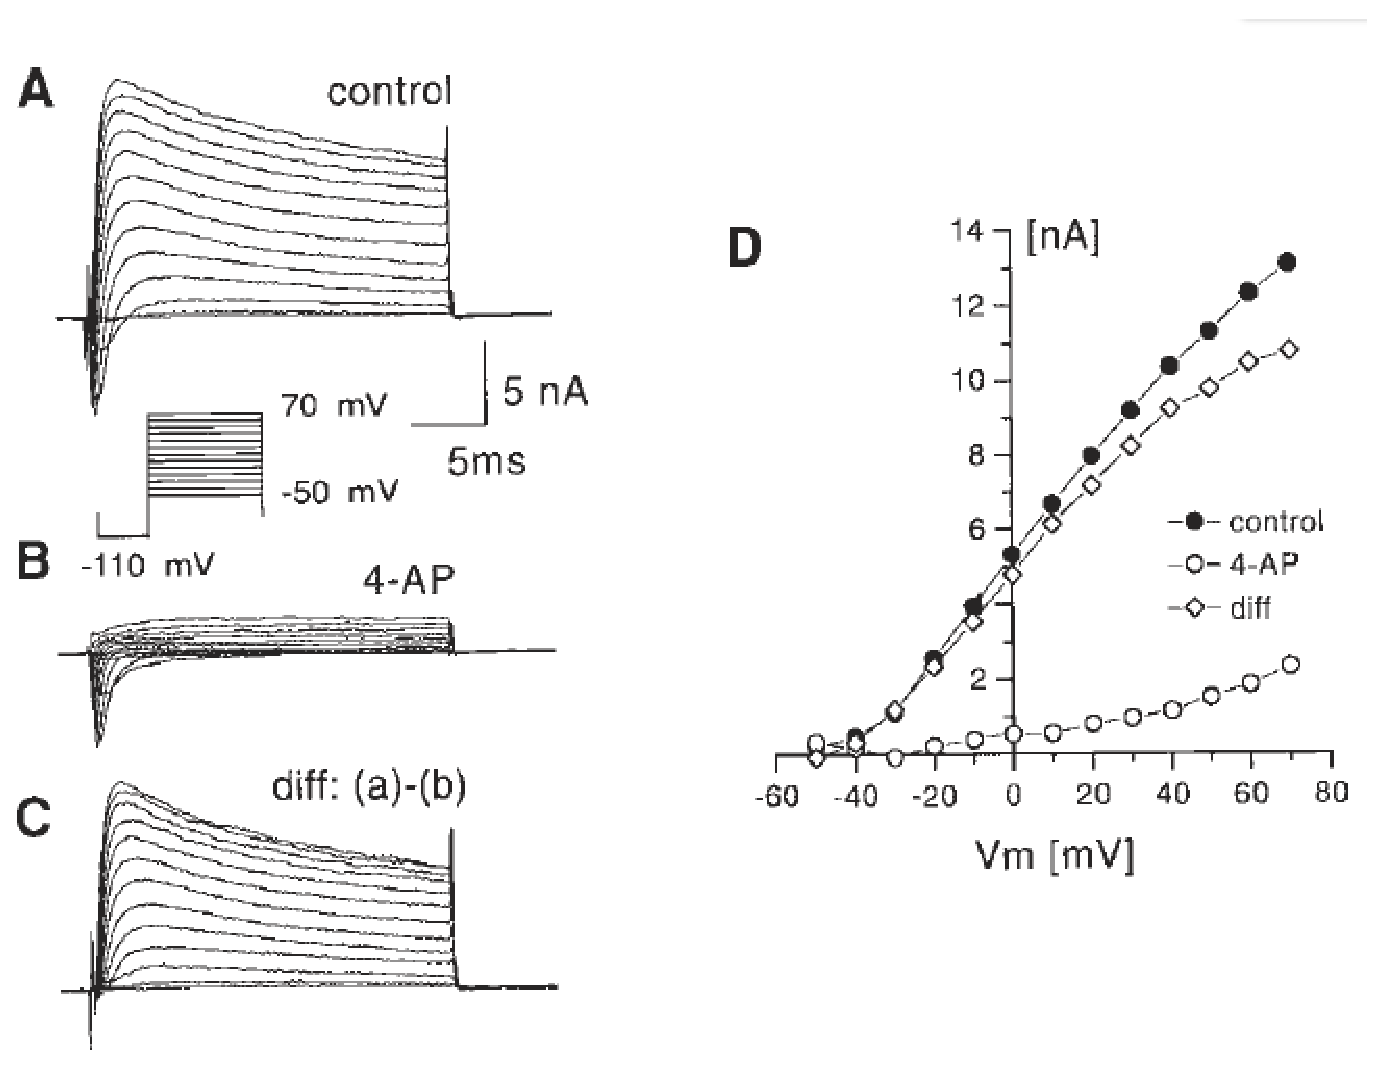
\includegraphics[height=4cm,
    angle=0]{./images/4-AP_Kcurrent.eps}}
\caption{(A) traces recorded from a spinal cord astrocyte using stepprotocol
indicated in inset; (B) recording from the same cells (with same
stimulus protocols) at 2 min after application of 2 mM 4-AP to block
4-AP-sensitive K+ current; (C) the 4-AP-sensitive K+ current as the result of
subtraction (B) from (A); (D) The I-V curve (Sect.\ref{sec:I-V-curve})}
\label{fig:4-AP_Kcurrent}
\end{figure}


Kv4 channels are assembled into macromolecular complexes (An et al., 2000;
Shibata et al., 2003). Quantitative PCR analysis of iSPNs separated by FACS
revealed that mRNAs for Kv4.1, Kv4.2, Kv4.3 subunits and auxiliary KChIP and DPP
subunits were expressed. In strial neurons, Kv4.2 subunits were much more
abundant in iSPNs (D2-MSN - Sect.\ref{sec:iSPN}) than either Kv4.1 or Kv4.3
subunits.

\textcolor{red}{\bf Modulators}: The Kv4.2 $\alpha$
subunit can be modulated by (1) protein-protein interaction with interacting
partners (Nakahira et al., 1996; Perez-Garcia et al., 1999; An et al., 2000;
Holmqvist et al., 2002; Nadal et al., 2003); (2) phosphorylation

\begin{itemize}
  \item protein-protein interaction:

NOTE: Many proteins that strongly interacted with the Kv4.3 N-terminal bait also
interacted with the N-terminal 180 amino acids of Kv4.2, but not with Kv1.1
  
\begin{enumerate}
  \item Kv $\beta$ subunits


  \item KChIP (K+ channel interacting proteins) - Sect.\ref{sec:KChIP}

Both KChIP1 and KChIP2, but not KChIP3/4, robustly associated with Kv4.2
subunits.
  
  \item dipeptidyl peptidase IV-related proteins 
\end{enumerate}

  \item bona fide substrate phosphorylation:
 
\begin{enumerate}
  \item extracellular signalregulated kinase (ERK)-mitogen-activated protein
  kinase (MAPK) and 
  
  \item PKA (Adams et al., 2000; Anderson et al., 2000) phosphorylate Kv4.2 at
  N-terminal and C-terminal cytoplasmic domains at sites Thr-38 and Ser-552,
  respectively - Sect.\ref{sec:PKA}. \textcolor{red}{Vm-dependent activation of
  Kv3.2 is decreased by PKA, PKC activation, i.e. 15mV shift } (Hoffman,
  Johston, 1998). IMPORTANT: requires KChIP3 co-expression (Schrader, Sweatt,
  2002)
  %%: found in hippocampal CA1 neurons and ventricular myocytes

\textcolor{red}{DATA}: PKA phosphorylation of synthetic peptide
\begin{itemize}
  \item at site N-terminal: $K_m$ = 294 $\muM$, and velocity $V_\max = $ 7.7
  $\mu$mol/min/mg.

NOTE: At high concentration of PKA, it has inhibition effect.
  
  \item at site C-terminal: $K_m$ = 133 $\muM$, and velocity $V_\max = $ 54.1
  $\mu$mol/min/mg.
\end{itemize}
NOTE: A well established PKA substrate, Kemptide has $K_m$ = 16 mM and Vmax
= 20.2 $\mu$mol/min/mg (at 30$^\circ$C).


This post-translational modifications have been shown to change both current
density and biophysical properties of A-type K+ current thoughts to be mediated
by Kv4.2 (Hoffman and Johnston, 1998; Yuan et al., 2002)

  \item CaMKII phosphorylate Kv4.2 at Ser438, Ser459 (Varga, Sweatt, 2004) 
\end{enumerate} 

\end{itemize}


\subsection{------  4-AP (microMolar range) sensitive K+ current: KAs
(D-current $I_D$): Kv1.2 - sensitivity to both $\alpha$-dendrotoxin
and low concentrations of 4-AP}
\label{sec:K+current_4-AP-sensitive-KAs}
\label{sec:KAs-current}
\label{sec:D-type-K+-current}

IAs (KAs) is a delayed-rectifier of fast-activation kinetics (D-current or
$I_D$) to distinguish it from KDR - Sect.\ref{sec:delayed-rectifier} which is a
non-A type current. 

\begin{mdframed}

$I_D$ was first described by Storm (1988) in hippocampal CA1 pyramidal neurons.
It was distinguished by its slow inactivation, sensitivity to (first) low
concentrations of 4-aminopyridine (IC50 = 40 $\muM$) (Storm, 1988; Wu and
Barish, 1992; Golding et al., 1999); and ability to delay the onset of AP firing
during long current steps.

A more recent criterion is its sensitivity to $\alpha$-DTX, which has been shown
to block the same slowly inactivating current as 50-100 $\mu$M 4-AP in
hippocampal (Wu and Barish, 1992; Golding et al., 1999) and cortical neurons
(Foehring and Surmeier, 1993; Locke and Nerbonne, 1997).
Bekkers and Delaney (2001) showed that D-current is reduced/blocked by either
100 $\muM$ 4-AP (aminopyridine) and 1-2mM $\alpha-$DTX (dendrotoxin,
Sect.\ref{sec:dendrotoxin}).
NOTE: $\alpha$-DTX is the toxic (antagonist) specific to D-current; but 4-AP
also affect A-type current KAf (Sect.\ref{sec:A-type-K+current}).

They presents mainly near the soma, also, their present is at low density.
The Kv1.2 subunit, probably in combination with other Kv proteins and Kv$\beta$
subunits, is thought to comprise $I_D$ channels (Coetzee et al., 1999).

\end{mdframed}

The channel activates {\it transiently} with a small depolarization in the {\it
subthreshold range} for membrane potential generation  and then quickly
inactivated during depolarizing pulses of duration~\citep{connor1971prf}.

KAs activates rapidly at subthreshold membrane potentials (spike threshold about
-45 mV in striatal neurons; and the channel open at about -65 mV), inactivates
over hundreds of milliseconds (i.e. non-inactivating or very large
inactivating time-constant), and is
\begin{itemize}
  
  \item selectively blocked by low concentrations of 4-AP (IC50 = 100 $\mu$M)
  (Surmeier et al. 1991, 1994).
  
  \item blocked by DTX (IC50 = 30 nM) (Surmeier 1991)
\end{itemize}

The classic KAs current (Nisenbaum et al., 1994) has been recently attributed to
Kv1.2 channels (Shen et al., 2004) - Sect.\ref{sec:Kv1.2}.

\begin{enumerate}
  \item Shen et al. (2004) assumed Kv1.2 form the classic KAs current
\end{enumerate}

{\bf IMPORTANT}: $\alpha$-DTX-sensitive channels are functionally different from
delayed rectifier IK channels; even though $\alpha$-DTX-sensitive channels
resemble IK channels both in their steady-state activation properties (Fig. 5D)
and their relatively slow kinetics (Bekkers, Delaney, 2001).

As $I_D$ is near soma, and little change of $I_D$ is sensitive to neuron's
excitability, it is likely that $I_D$ current plays the role of modulating spike
threshold in the axon. Such a role could be further enriched if $I_D$ is subject
to neuromodulation. Indeed, activation of metabotropic glutamate receptors has
recently been reported to accelerate the inactivation of $I_D$ in CA1 pyramidal
neurons, increasing neuronal excitability (Wu and Barish, 1999).

\subsection{--- Kv4.3}
\label{sec:Kv4.3-channel}

Kv4.3 is an A-type $\K$ channel subunits expressed strongly in basket cells
(Sect.\ref{sec:basket-cell}) and stellate cells (Sect.\ref{sec:stellate_cells})
but not in Purkinje cells (PCs) in adult cerebellum (Hsu et al., 2003) - see
also Masugi-Tokita (2007).


\subsection{A.3. myocyte (atrial + ventricular) Ito: Kv1.4, Kv4.2, Kv4.3}
\label{sec:A-type-K+current-myocyte}
%: $I_A$ (neuron) and $\Ito$ (heart)

A-type channels in muscle (myocyte) are encoded by Shaker gene
(Sect.\ref{sec:Kv1-channels}).
\textcolor{red}{In atrial and ventricular cardiac cells, A-type current are
present and are called with a different name ``transient" outward current} (Ito
or $\Ito$) (Sect.\ref{sec:Ito-current}), {\it or rapidly inactivating K current
or fast transient K current} \citep{wang1998, wang1994, cai2007}. In cardiac
cells, there are two genes to encode A-type current: fast (rapid) component and
slow component; thus giving the two other names $\Itof, \Itos$. 
% \begin{itemize}
%   \item slow component: Kv
% \end{itemize}
Ito is encoded by A-type K+-channel genes such as Kv1.4, Kv4.2, and Kv4.3.

\begin{mdframed}
\textcolor{red}{It is often not easy to distinguish A-type K+ current and
delayed rectifiers K+ current (Sect.\ref{sec:delayed-rectifier}). That's why in
cardiac cells, A-type current is also called delayed-rectifier IK current in
some publications}.
\end{mdframed}

In contrast to neuronal A-type currents
(Sect.\ref{sec:A-type-K+current-neuron}), Ito channels are available at resting
membrane potentials, and thus is predominantly responsible for the initial
repolarization (phase 1) of the cardiac action potential,
Fig.\ref{fig:ion_channel_roles_AP}.

The distribution of Ito within the myocardium is nonuniform and contributes
toward regional variations in action potential waveforms. In cardiac myocyte,
A-type current Ito has
\begin{enumerate}  
   \item early activation (with measurable thresholds typically between -45 and
   -60 mV) compared to $I_K$ ($> -40$mV).

   \item quickly inactivate, i.e. the steady-state inactivation complete
  at -40mV

The short time of opening can cause an early  phase of incomplete
repolarization, but do not contribute significantly to the repolarization from
the plateau phase. This creates a top-notch shape in the cardiac AP.
   
   \item repolarization to potentials negative to -50 mV is typically required
   for restoration of channel availability
   
   \item Inhibition by  
\begin{enumerate}
  \item 4-aminopyridine (4-AP) at mM concentration -
   Sect.\ref{sec:4-AP})
  \item Cs and TEA (internal)
\end{enumerate}
   
   \item It is insensitive to extracellular tetraethylammonium (TEA) ions are
   considered to be pharmacological hallmarks of A-type currents (although
   notable exception exists).

\end{enumerate}

\begin{figure}[hbt]
  \centerline{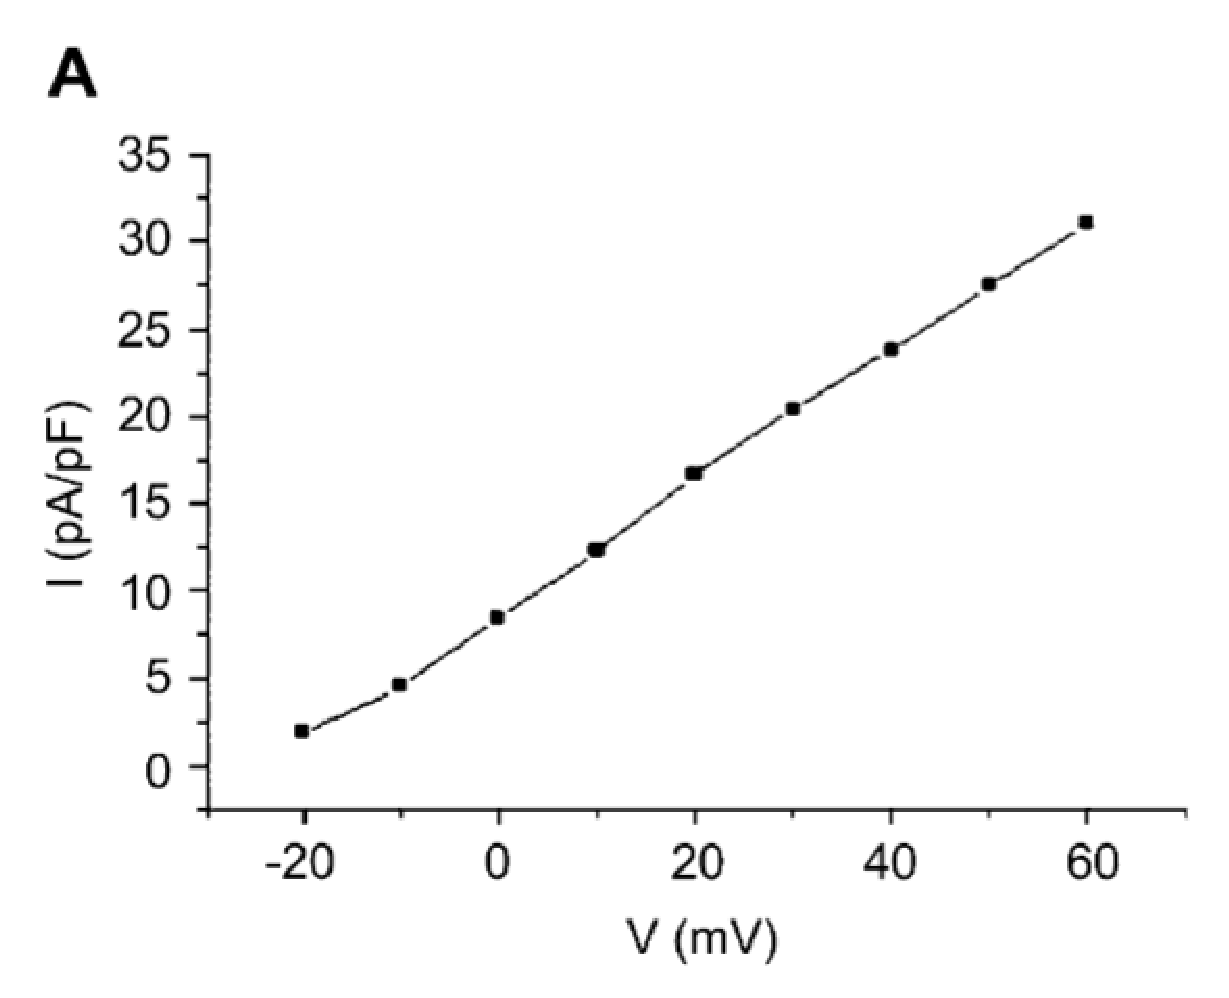
\includegraphics[height=4cm,
    angle=0]{./images/IVcurve_Ito.eps}}
\caption{I-V curve of the transient outward postassium current $\Ito$ obtained
from an isolated canine left ventricular epicardial myocyte
\citep{kornreich2007}}
\label{fig:IVcurve-Ito_canine}
\end{figure}


Its potent properties are:
\begin{enumerate}
  \item  Ion selectivity:
$\K \gg \Na$. 

  \item The current can be fitted - Sect.\ref{sec:A-type-K+-model}
  
\end{enumerate}


\subsection{A.4. smooth muscle cell}
\label{sec:A-type-K+current-smoothmuscle}

A-type current was also found in vascular smooth muscle cells
\citep{amberg2003}. In contrast to the A-type currents of the myocardium
(Sect.\ref{sec:A-type-K+current-myocyte}), the physiological function of A-type
currents in vascular myocytes has not been fully clarified.
However, it is suggested that the physiological function of A-type currents in
smooth muscles may be related to the maintenance of membrane potential and
regulation of excitability.


A-type currents have been identified in vascular smooth
muscle cells of the rabbit (portal vein, pulmonary artery, aorta), rat
(pulmonary artery, renal resistance artery), and human (mesenteric artery).
A-type currents have been identified in genitourinary (GU) smooth muscle cells
of the guinea pig (ureter, seminal vesicles, and vas deferens), rabbit (vas
deferens), rat (myometrium), and human (myometrium).
A-type currents are also present in gastrointestinal (GI) smooth muscle cells of
the mouse (fundus, antrum, jejunum, and colon), rat (ileum), guinea pig (colon),
and opossum (esophagus), and a "transient delayed rectifier" has also been
characterized in the human esophagus.





\subsection{B. non-A current (Delayed rectifier $\Kdr$): IK2, IKr, IKs}
\label{sec:delayed-rectifier}


Delayed rectifier $\Kdr$ (non-''A'' voltage-dependent K channels) is (1) an
outward $\K$ current (Sect.\ref{sec:K_outward-rectifier}) and (2)
voltage-dependent (Sect.\ref{sec:Kchannel_Vm-dependent}); yet open slowly, i.e.
with a delay after transmembrane potential depolarized.
The current is important for repolarizing the AP.

At least five gene families are known to code for subunits having delayed
rectifier-like properties (Kv1, Kv2, Kv3, eag, KCNQ) (Pongs, 1992; Shi et al.,
1997, 1998; H. Wang et al., 1998)

Sect.\ref{sec:Ik_HodgkinHuxley-axon} describes the history of K(dr) current.
Basec on the kinetics, it can be divided into three components of the delayed
rectifier $I_\Kdr$, as given below.
There's also a third type of delayed-rectifier, called ultra-rapid delayed
rectifier current IKur ($I_\text{Kur}$) \citep{li1996}.

\begin{enumerate}

  \item IK2 - Sect.\ref{sec:IK2_current}
      
  \item $I_\Kr$, $K_f$ or $K_r$ or HERG channel \footnote{we use HERG
  name when refering to human cardiac cell}, Fig.\ref{fig:Kcurrent_IKs_IKr} -
  Sect.\ref{sec:IKr_current}
  
  $I_\Ks$ has a linear I-V relationship, and $I_\Kr$ is preferentially blocked
  by class III antiarrhythmic compounds \citep{sanguinetti1997}.

  \item $I_\Ks$ or $K_s$ - Sect.\ref{sec:IKs_current}.


\end{enumerate}
When any of the two genes encoding the two later currents is defective, it may
give rise to 2 different types of long QT syndrome. 
Class III antiarrhythmic drugs inhibit $K_r$ but not $K_s$ channels. 

TEA applied internally blocks $I_K$ currents, A-type currents and Ca-activated K
currents also. Extracellular ATP was found to increase $I_\Kdr$ current in
guinea-pig ventricular myocytes \citep{matsubayashi1999}.


\subsection{-- Ik : IK2(Ik), IKr(Ix1), IKs(Ix2)}
\label{sec:Ik_HodgkinHuxley-axon}
\label{sec:IK2_Purkinje-fiber}
\label{sec:IKx1_Purkinje-fiber}
\label{sec:IKr_Purkinje-fiber}
\label{sec:IKs_Purkinje-fiber}
\label{sec:IKx2_Purkinje-fiber}

\begin{mdframed}
The concept of an ($V_m$-dependent) outward delayed rectifier $\K$ current
$I_\k$ was first given in Hodgkin-Huxley modeled (Sect.\ref{sec:I_Kdr}) in
their experiment on axon in that the conductance shows a significant delayed
before rising under voltage clamp protocol.

In Hodgkin-Huxley model (1952), it has only one potassium current component, so
they used \textcolor{red}{the notation $I_\text{K}$ which is now obsolete} as
better notation is recommended when multiple types of potassium current is
added. They activate with a delay upon the depolarization of the membrane
potential, and rises slower than the Na current~\citep{hodgkin1952cmc}. In this
model, the current $I_\k$ is responsible for the repolarization of the AP, i.e.
terminating the AP. This K current is not activated by a rise in internal
\ce{Ca^2+} concentration.

Later on, in the model developed for Purkinje fiber, the concept was revised
with three outward $\K$ currents. \textcolor{red}{The role of $I_\k$ in HH model
is substituted by $I_{K2}$ in later models}, so that the two other outward K+
current components can be added: 
\begin{itemize}
  \item  the fast component $I_\Kr$ (early called $I_{x1}$) and 

  \item the slow component $I_\Ks$ (early called $I_{x2}$)
  \citep{difrancesco1981nip, sanguinetti1997}.
\end{itemize}

\textcolor{red}{"A" current (Sect.\ref{sec:A-type-K+current}) and
delayed-rectifier currents are similar (in terms of kinetics) in cardiac cells
(but not in neurons). So in cardiac cells, some papers interchangebly uses the
two terms}: with (guinea pig), the classical delayed rectifier curent IK are
called IKr (rapid IK) and IKs (slow IK); while in human and canine we use the
term $I_\tof, I_\tos$ which are indeed A-type current
(Sect.\ref{sec:A-type-K+current}).

\end{mdframed}



\subsection{-- IK2 }
\label{sec:IK2_current}

(\textcolor{red}{current notation}: $I_\text{K2}$, $I_\text{K-DR}$,
$I_\text{k,DR}$) develops slowly ($\tau_h \approx 200-2000$ms) 

The outward current during the plateau phase to counter the inward current
caused by LCC and NCX. In the cardiac myocyte, the resulting net current is
slightly outward and causes a slow rate of repolarization from the plateau to
-20mV. When the membrane potential repolarize enough, the increase
inward-rectifier (Sect.\ref{sec:Kir_family}) become actives and can rapidly
bring the membrane potential back to the resting level -80mV.

\textcolor{red}{$I_{K2}$}: The channels display in bursting behavior . Ion
selectivity: T1$^+$ > K > RB > \ce{NH4} $\gg$ $\Na$. This type of channels
is blocked by (not completely, but at various degree)

\begin{enumerate}
\item divalent cations in the cell, like $\Ca$, $\Ba$
\item 4-aminopyridine (4-AP): block equally from outside or inside of
  the cells
\item Tetraethylammonium (TEA) in the cell: block differently, suggesting two
  different types of binding sites (externally applied blocks some K
  channels, but not other K currents). 
\item Cs ions
\end{enumerate}


\begin{framed}

{\it Drosophila} provides a unique tools of mutant analysis to study ionic
channels. {\it Shab} gene is the exclusive gene underlying delayed rectifier
currens in both muscle and neurons \citep{tsunoda1995}. 
The current can be fitted using Sect.\ref{sec:Boltzmann-equation}
\end{framed}

\subsection{-- $I_\Kr$ (rapidly delayed-rectifier): Kv1.2}
\label{sec:IKr_current}
%\subsection{Rapidly delayed-rectifier $I_\Kr$ channels}
\label{sec:Kv1.2}

% (notation: IKr, IKf) 

\begin{enumerate}
  \item Kv11.1 channel: 

The rapidly delayed rectifier current $I_\Kr$ found in ventricular
myocytes of many species, including neonatal mice, is the
summation of the currents through inward-rectifying Kv channels
(Kv11.1)~\citep{mazhari2001,clancy2001,oehmen2002,fink2008}.

In human the gene to encode the Kv11.1 channels in called hERG gene, giving the
name hERG channels. It plays an important role in regulating cardiac AP. HERG
channels have the same kinetics of $I_\Kr$ in mice, except for more negative
activation \citep{liu2004}. 
  
  \item 
\end{enumerate}


$I_\Kr$ has a bell-shaped of I-V relationship. The rapid component is given in
Fig.\ref{fig:IVcurve-IKr}. The slope become negative about 0mV when assessed
with 4-s pulses. The blocker of $I_\Kf$ is E-4031 (at 3$\muM$) and sotalol.

 
\begin{figure}[hbt]
  \centerline{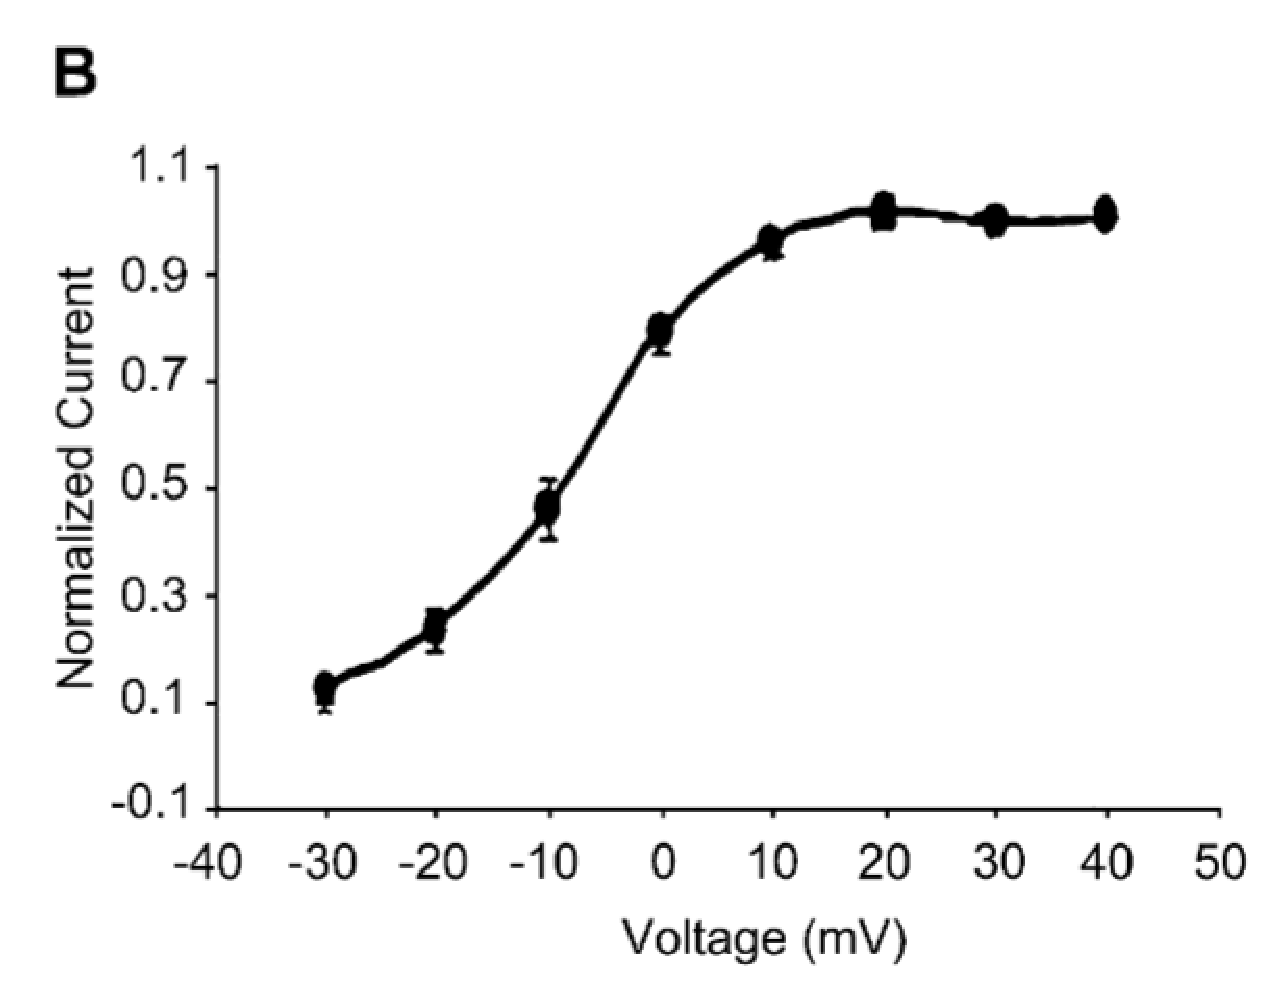
\includegraphics[height=4cm,
    angle=0]{./images/IVcurve_IKr.eps}}
\caption{I-V curve with normalized current for the rapid component of the
delayed rectifier $\K$ current (IKr) by overexpression of HERG in canine
ventricular myocyte \citep{hua2004}}
\label{fig:IVcurve-IKr}
\end{figure}

EXPERIMENT: The membrane is clamped with a high voltage (+20mV) for a long
enough period to permit $I_\Kr$ to reach the steady-state.
Then the membrane is pulsed to a new testing potential, from that we measure the
peak current, Fig.\ref{fig:IKr_peakcurrent}. Peak current was determined with
($\Circle$) or without ($\CIRCLE$) a hyperpolarizing interpulse. The magnitude
with a hyperpolarizing test pulse (at $\Circle$) is the measurement of
instantaneous I-V relationship in the absence of channel inactivation.

\begin{figure}[hbt]
  \centerline{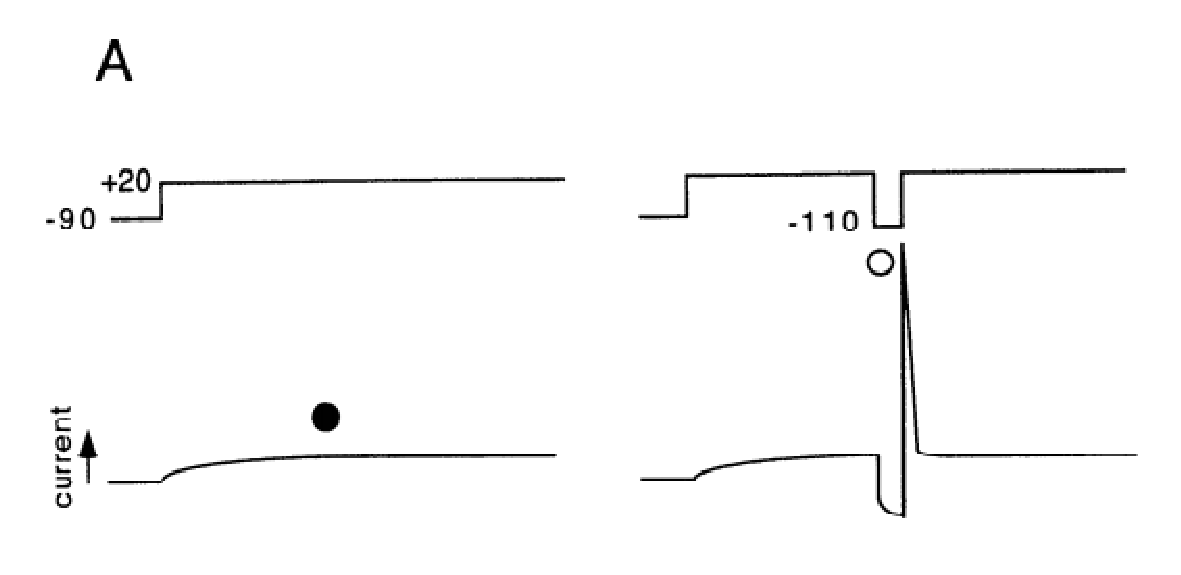
\includegraphics[height=5cm,
    angle=0]{./images/IKr_Sanguinetti1997.eps}}
  \caption{Using test pulse of -100mV to emulate fast channel inactivation
  which cause rectification of $I_\Kr$ channel. The brief interpulse allow the
  channel to recover from inactivation to open state.}
  \label{fig:IKr_peakcurrent}
\end{figure}

\subsection{-- $I_\Ks$ - the slow-component of delayed-rectifier current}
\label{sec:IKs_current}

 \citep{iost1998, li1996}
 
$I_\Ks$ is formed by KvLQT1 and the $\beta$-subunit called minK
(Sect.\ref{sec:minK-subunit})  \citep{barhanin1996, sanguinetti1996}. $I_\Ks$
responds to $\beta$-adrenergic stimulation (to enhance
4-6x)\citep{kurokawa2001}. This can be physiologic or phatologic significance.
Example: under tachycardia, the time between beats is shortened which may
threaten coronary flow that occur mainly in diastole. Hence, with
$\beta$-adrenergic stimulation, it shorten the AP to give enough time for
adequate coronary flow. However, under long QT syndrome, this sympathetic
stimulation can accelerate the advent of the next depolarizing, leading to
serious arrhythmias and cardiac death.


\subsection{-- IKur current (Kv1.5)}
\label{sec:IKur_current}

The ultra-rapid activating delayed rectifier K(+) current (I(Kur)), carried by
Kv1.5 channels, is a major repolarizing current in human atria, but seems to
play no role in the ventricle.

Its role in restoring sinus rhythm has been under studied \citep{tamargo2009}
 

\subsection{4-AP resistant (and TEA-sensitive), persistant K+ current:
KRP}
\label{sec:KRP}

Depolarization-activated, calcium-independent potassium
(K+) currents has 2 components: transient and persistent components. In this
section, we focus on the persistent part - KRP.

The persistent component of K+ outward current called KRP 

KRP is resistant to 4-AP (i.e. 10 mM 4-AP only reduces 40-50\% of KRP), yet it
is sensitive to TEA.

NOTE: 4-AP also blocks the A-current (Storm, 1993), D-current
(Sect.\ref{sec:D-type-K+-current}). Partial blockage of A-current requires
micromolar 4-AP.

This persistent K+ current as 2 components, based on the effect of TEA
(tetraethylammonium - Sect.\ref{sec:TEA}).
The concentration-response curve is fitted by the sum of two exponential curves
\begin{equation}
I = \frac{I_\max}{1 + \frac{[\TEA]}{\text{IC50}_1} } +
   \frac{1- I_\max}{1 + \frac{[\TEA]}{\text{IC50}_2} }
\end{equation}
suggesting a high and low-affinity binding sites presents on the channel.

TEA concentration:
\begin{itemize}
  \item IC50(1, high-affinity site) = 125$\muM$ block 23\% of blockable current
  
  
  \item IC50(2, low-affinity site) = 5.9 M blocks 77\% of blockable current
  
  25mM of TEA blocks 90\% of the current
\end{itemize}

PROPERTIES:
\begin{enumerate}
  \item relative insensitive to 4-AP; but sensitive to TEA  (as given above)

  \item relatively hyperpolarized membrane potential for activation
  
  Unlike the other persistent K+ current, i.e. KAs (Sect.\ref{sec:KAs-current})
  in many other cell types, KRP activates at relatively hyperpolarized membrane
  potentials (approximately -70 mV; while KAf/KAs is at -40mV); and the
  inactivation is at more depolarized potential (-55mV; while KAs is at -100mV
  and KAf is at -60mV). The slope for inactivation is steeper for KRP (6mV for
  KRP; and 19mV for KAf).
  
  The Boltzmann function describing activation had a half-activation Vmh = -13
  mV, with slope Vcm = 12 mV.

  \item slow kinetics of activation at $\Vm$ at or below the spike threshold
  
  
  \item slow kinetics of inactivation
  
  
\end{enumerate}


\subsection{KCNQ current: Kv7.2, Kv7.3)}
\label{sec:Kv7.x}
\label{sec:KCNQ}

{\it KCNQ} genes encode five Kv7 K+ channel subunits
\begin{enumerate}
  \item Kv7.1
  
  \item Kv7.2
  
  \item Kv7.3
  
  \item Kv7.4
  
  \item Kv7.5
\end{enumerate}
Among them, four forms (Kv7.2, Kv7.3, Kv7.4 and Kv7.4) are expressed in the
CNS.

Kv7.2 and Kv7.3 are the principal molecular components of slow voltage-gated
M-channel. In some cases, an ``M'' current is part of a ``delayed rectifier''
- Sect.\ref{sec:M-current}. It regulates firing frequency, e.g. in adaption
(Sect.\ref{sec:adaptation-AP}).



\subsection{``S'' current}

The current is outward rectifying with weak $V_m$-dependent. The channel is
blocked by cAMP-dependent protein kinase phosphorylation, which is the result
from [cAMP] increases produced by serotonin \citep{klein1982}.



\subsection{Maxi-K current}

This current is voltage-dependent $[\Ca]_i$-regulated current
(Sect.\ref{sec:MaxiK-current}).

\subsection{TREK-1}

Sect.\ref{sec:TREK-1-channel}

\section{K(Ca) or KCa channels: 6TM/P}
\label{sec:Kchannel_Ca-activated}
%\subsection{K(Ca) family}
\label{sec:K(Ca)_family}

$\Ca$-dependent potassium channel (K(Ca) channels) were first characterized in
red blood cells, where their activation leads to membrane hyperpolarization and
cell shrinkage, i.e. it causes an outward current. In CNS, the first K(Ca)
channels described were those in mollusc neurons and cat spinal motor neurons.

\textcolor{red}{NOTE}: Some $\Ca$-activated K channels also show
voltage-dependent. Like any other calcium-sensitive processes, $g_{\ce{Ca}}$
obtains voltage dependence from the voltage dependence of \ce{Ca^2+} entry.
NOTE: BK(Ca) channels are a special member of Kv-subfamily
(Sect.\ref{sec:Kv_channel}).

In frog sympathetic neurons, 3 different $\Ca$-dependent $\K$ current
\begin{enumerate}
  \item {\bf fast-activating, non-inactivating current} $I_C$ 
  
  The channel is blocked by TEA - Sect.\ref{sec:TEA}
  (frog ganglia: Adams et al. 1982; hippocampus: Brown \& Griffith, 1983a;
  Lancaster \& Adams, 1986);

  \item fast transient TEA-sensitive current
  
  (frog ganglia: MacDermott \& Weight, 1982, Brown, Constanti \&
  Adams, 1982; hippocampal CA3 cells: Zbicz \& Weight, 1985; CAl cells: Storm,
  1986a)

  \item {\bf slow, non-inactivating TEA-resistant current} $I_\AHP$ - this
  current underline the slow after-hyperpolarization (AHP) in frog ganglia 
  (Pennefather, Lancaster, Adams \& Nicoll, 1985) and hippocampal pyramidal cells
  (Lancaster \& Adams, 1986).
  
\end{enumerate}

In mammals, the channel is similar to Slo (Sect.\ref{sec:SLO-channel}) There are
different types of $\Ca$-activated Slo-like $\K$ channels, and they are found in
different types of cells \citep{blatz1987}. They were first found in red blood
cells, under the name Gardos channel (Sect.\ref{sec:Gardos-channel}) where the
rise in $[\Ca]$ opens the Gardos channel causing potassium loss and cell
dehydration.


SK channels and IK channels are more sensitive to $\Ca$ than are BK channels;
and only BK channels has both $[\Ca]_i$-dependent (as a modulator) and
$V_m$-dependent (as an activator). Even though there are several types of
Ca-activated K channels, the first two of them are well characterized:
\begin{enumerate}
  
  \item BK channels or Maxi-K channel or TEA-sensitive K(Ca) channel
  (KCa1.1, $I_{\ce{K(Ca)}}$, $I_\text{K,Ca}$, $I_C$) -
  Sect.\ref{sec:MaxiK-current}
  
  Large unitary conductance (200-300 pS).
  
  \item Small-K channel (SK) or slow AHP\footnote{AHP = afterhyperpolarization}
  K(Ca) channels ($I_{AHP}$) - Sect.\ref{sec:SK_current}. 
  
  The smaller unitary conductance is 2-25pS. In contrast to BK channel,
  $I_{AHP}$ is a very small current with little-voltage dependent, yet higher
  \ce{Ca^2+} dependent and is not blocked by TEA.
  
  \item IK (Intermediate-conductance $\Ca$-activated
  K current) \ce{K+} channel, with conductance 20-85 pS 
  %25-100pS
  (Sect.\ref{sec:IK_current})
  

  \item Others: KCa4.1 (Slack, Slo2.2), KCa4.2 (Slick, Slo2.1) , KCa4.3 (Slo3)
\end{enumerate}




\subsection{BK current (or Maxi-K, KCa1.1, Slo1-current, Slo-like channel):
large conductance (activated by $V_m$, modulated by $[\Ca]_i$)}
\label{sec:MaxiK-current}
\label{sec:BK-current}
%\subsection{Slo-like channel}
\label{sec:SLO-channel}

NAMES: KCa1.1, BK, Slo1, Maxi-K, KCNMA1.

The large conductances of the single channel (200-300pS) was called Big
Potassium (BK) channel by \citep{marty1983} (in chromaffin cells) or 'Maxi-K'
channels by \citep{latorre1983}. This large conductance makes the channel very
effective in hyperpolarizing the membrane potential, i.e. a major contribution
to fAHP (Sect.\ref{sec:AHP-fast}). 


\textcolor{blue}{BK(Ca) channels are found ubiquitously in almost every cells,
except heart myocytes}.
In neurons,BK channels colocalize with calcium channels, shape action potential
waveforms and regulate transmitter release.

\begin{mdframed}


Slo-like potasium channels were first cloned in {\it Drosophila} (Elkins et al.,
1986: Atkinson et al., 1991), and form large conductance BK-type channels
(Sect.\ref{sec:BK-current}).
This class can be divided into three subfamilies, typified by the vertebrate
genes mSlo (Slo-1), Slack (Slo-2) and mSlo-3 (Slo-3).
\begin{enumerate}
  \item Slo-1 (mSlo) gene (BK current, Maxi-K current -
  Sect.\ref{sec:MaxiK-current}):  expressed in brain, various muscles
  
  control the myogenic tone of arterial and airway smooth muscle, and are also
  key regulators of neurotransmitter release in vertebrate.
  
  Slo-1 mutations were also found to increase the quantal content of (1) release
  even in a wild-type (unc-64+) background; and (2) evoked EPSC four-fold. 
  
  \item Slo-2 gene in {\it C. elegans} (in vertebrate it is called Slack gene): 
  expressed in brain, various muscles
  
  Slo-2 genes are sensitivity to both intracellular calcium and chloride ions
  (Yuan et al., 2000); while in mammels, sodium and chloride ions co-activate
  Slo-2 channels. This may be an evolutionary adaption reflecting the absence of
  the classical voltage-dependent sodium channel in C. elegans. 
  
  \item Slo-3 (mSlo-3) gene: 
\end{enumerate}


\begin{mdframed}

The gene to encode the $\alpha$ subunut of BK channel is {\it Slo} (or Slo1 to
distinguish with newer discovered genes), as the primary sequence, first cloned from {\it Drosophila}
(flight muscle mutation called {\it Slowpoke}).
For this reason the $\alpha$-subunit is called {\it dSlo})
\citep{kaczorowski1996}. The genes to encode the BK channel in other species, in
mouse = {\it mSlo}, and in human = {\it hSlo} \citep{gribkoff2001}.

There are other newly identified genes ({\it Slo2, Slo3}) which show a close
analogies to {\it Slo} gene. 
\end{mdframed}

\end{mdframed}
 
Maxi-$K_\ca$ channels is the tetramer of 4 $\alpha$ subunits, each has 7
TM domains, Fig.\ref{fig:MaxiK_channel} \citep{toro1998}, with the newly
discovered transmembrane domain S0 is an exoplasmic N-terminus, and is suggested
to be critical for $\beta$-subunit modulation, Fig.\ref{fig:MaxiK_channel}.
The channels display two phenotypical types: type I
(Sect.\ref{sec:BK(Ca)-type-I}) and type II (Sect.\ref{sec:BK(Ca)-type-II})
\citep{calderone2002}.


Although the pore-forming subunit ( $\alpha$ subunit) is encoded by a single
gene, it has four tissue-specific accessory subunits, $\beta$1
through $\beta$4. 
\begin{enumerate}
  \item $\beta$1 subunit primarily distributes in smooth muscle cells

Association of the beta-1 subunit with the BK channel increases the apparent
Ca2+ sensitivity of the channel and decreases voltage dependence, i.e. shift
half-voltage activation to the right.

  \item $\beta$2 is found in  various endocrine cells, including pancreas and
  adrenal chromaffin cells, and in the brain, including hippocampus.

Association of beta-2 subunit cause, following activation of MaxiK current,
persistent inactivation.
  
  \item $\beta$3 subunit is found in smooth muscle (to control smooth muscle
  tone) and is also neuronally expressed
  
Association of beta-3 subunit  partially inactivate or slightly decrease the
activation time of MaxiK alpha subunit currents.  At least four transcript
variants encoding four different isoforms have been found for this gene.

  \item  $\beta$4 subunits are most exclusively expressed in the brain. 

Association of beta-4 subunit slows activation kinetics, leads to steeper
calcium sensitivity, and shifts the voltage range of current activation to
more negative potentials than does the beta 1 subunit.

\end{enumerate}
% e.g Kv$\beta$1.1 mediates fast N-type
% inactivation.
% 
% \begin{enumerate}
%   \item $\alpha$: Slo1 -  only composed of the pore-forming subunit
%   \item $\alpha$-beta?: Large conductance Ca2+-activated K+ channels
%   \item $\alpha$-beta?: Maxi-K
%   \item $\alpha$-beta?: BK or BKCa
%   \item $\alpha$-beta?: KCa1.1
% \end{enumerate}




\begin{figure}[hbt]
  \centerline{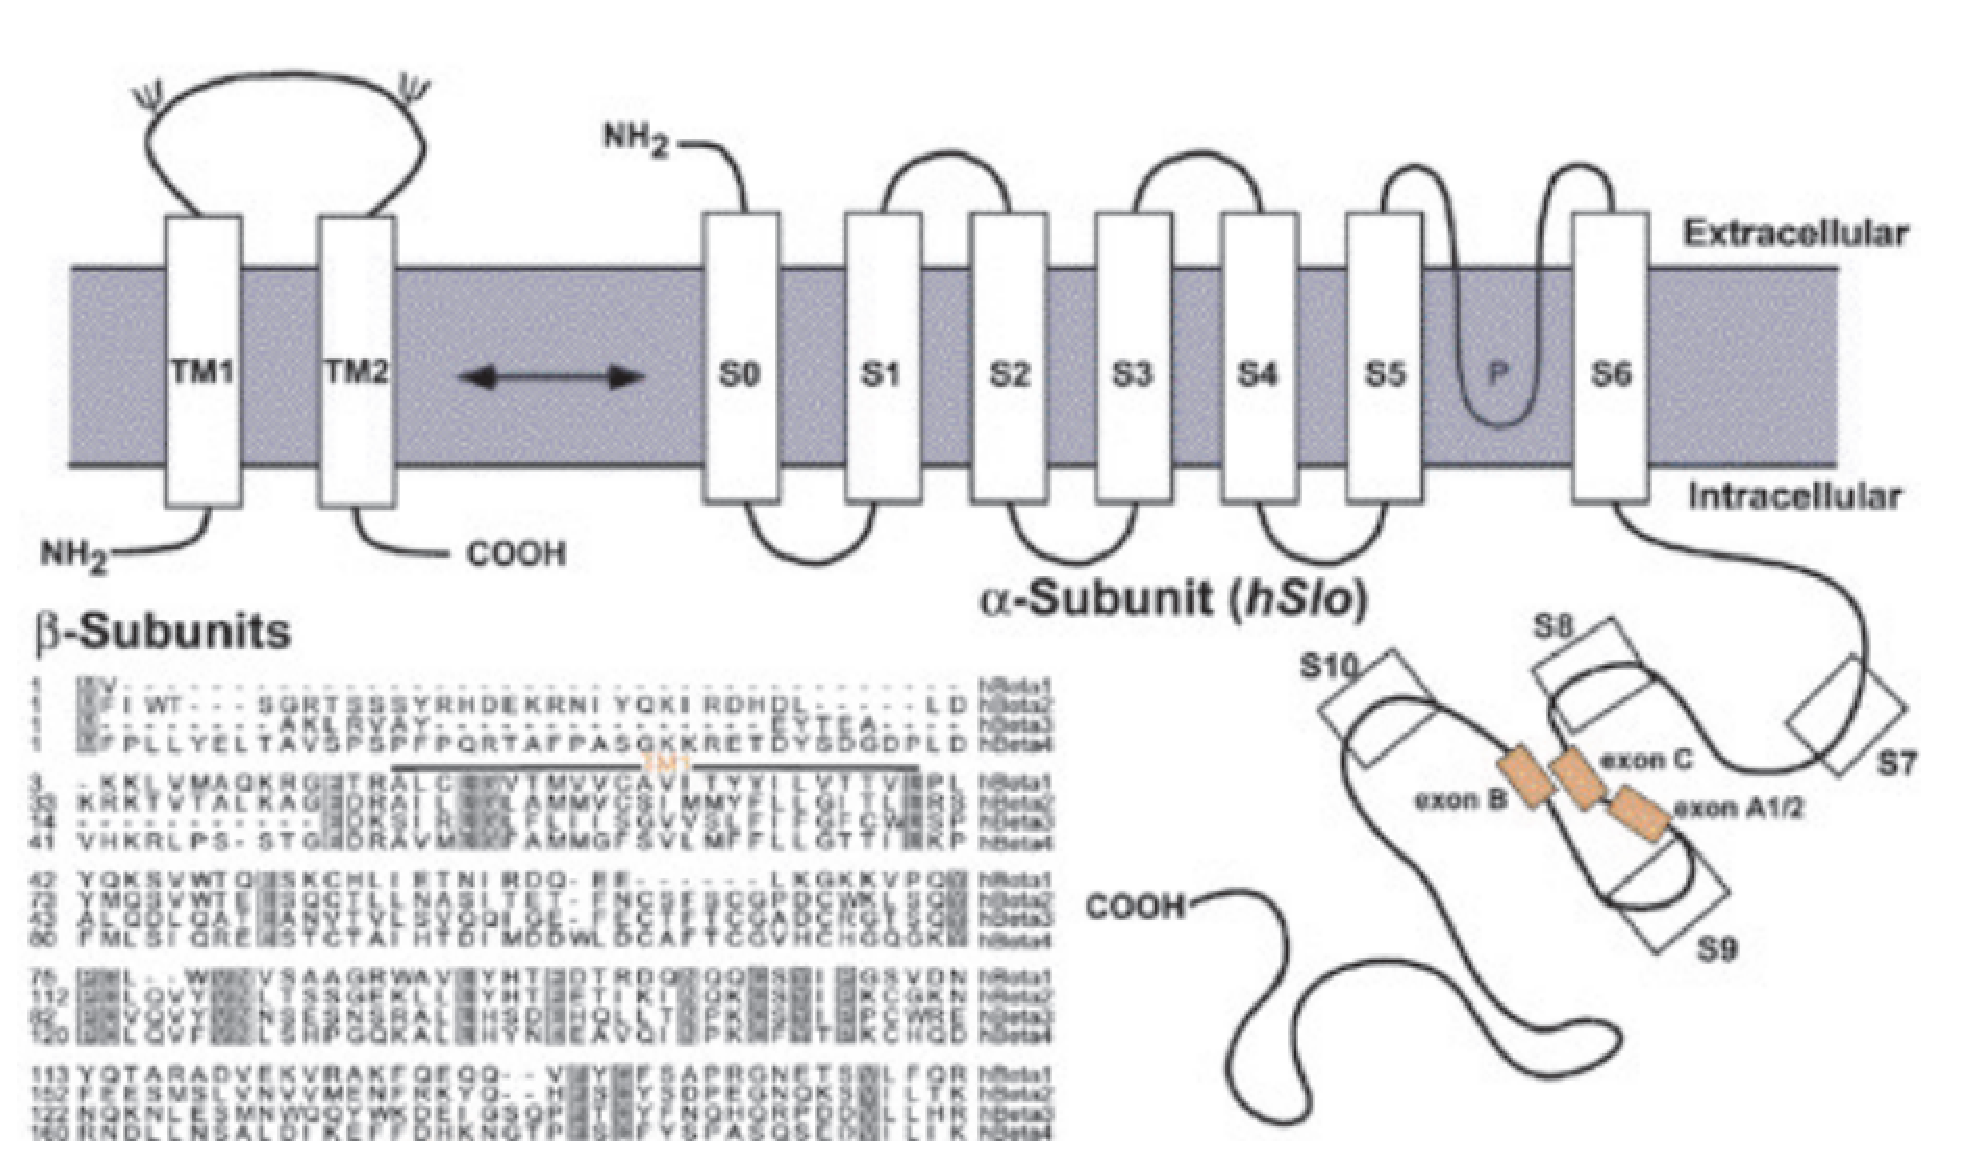
\includegraphics[height=5cm,
    angle=0]{./images/Maxi-K_channel.eps}}
  \caption{Schematic representation of a maxi-K channel protein including both
  the $\alpha$ and $\beta$ subunits. The {\it Slo} $\alpha$-subunit has 7
  transmembrane domain (S0-S6), a pore domain (P), and a long cytoplasmic tail
  containing 4 additional hydrophobic segments S7-S10. \citep{gribkoff2001}}
\label{fig:MaxiK_channel}
\end{figure}

Expression studies suggest that $\beta$2 and $\beta$4 are the principle
$\beta$ subunits expressed in central neurons, Fig.\ref{fig:BK(Ca)-channels}.
\begin{itemize}
  \item S2, S4: voltage-sensor

\label{sec:RCK-domain-BK-channel}

  \item RCK domain, Ca2+ bowl domain: $\Ca$-binding sites to control the
  conductance of $\K$ ions
  
  RCK domain control the conductance of \ce{K+} of the eukaryotic  BK \ce{K+}
  channel subfamily.
 
\end{itemize}


\begin{figure}[hbt]
  \centerline{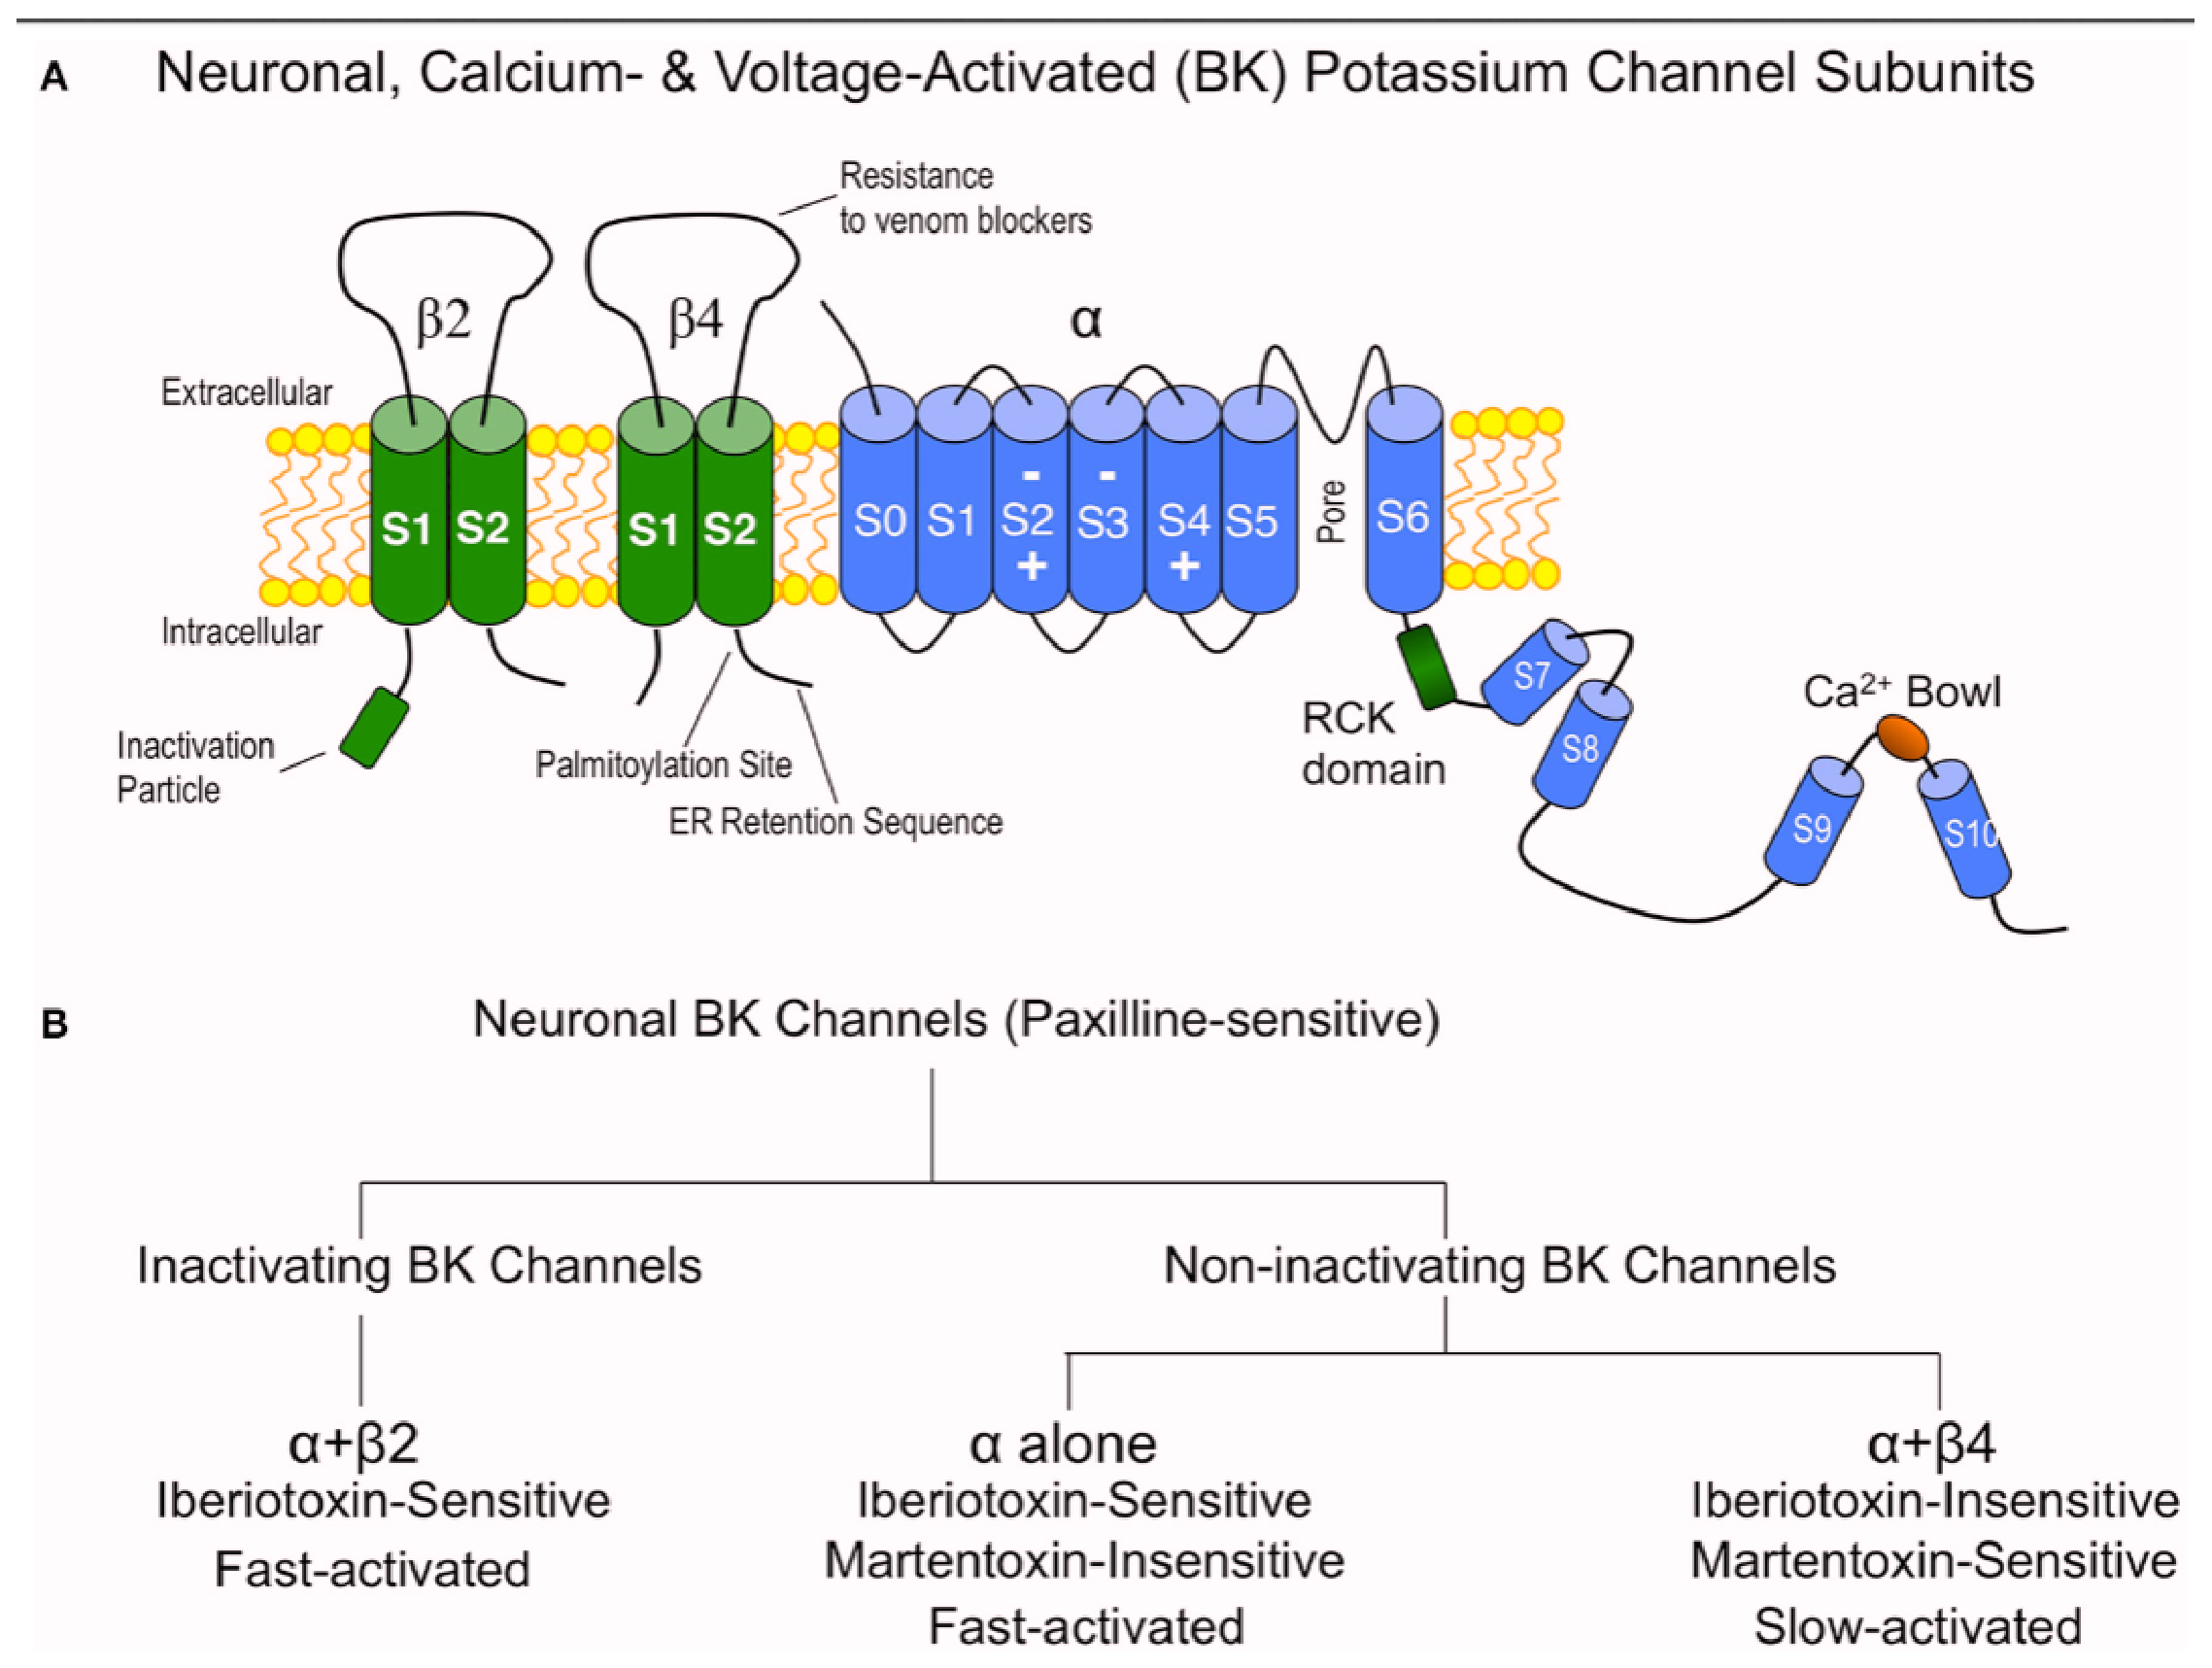
\includegraphics[height=5.4cm,
    angle=0]{./images/BK(Ca)-channels.eps}}
\caption{$\beta$2 confers fast-type inactivation; $\beta$4 contains residues
that confers venom torin-resistance. () Flow chart of neuronal BK channel
pharmacology and gating properties}
\label{fig:BK(Ca)-channels}
\end{figure}

\textcolor{red}{Blockers}:
paxilline (2-10$\muM$) indiscriminately blocks both type I and type II BK
channels (Hu et al., 2001).
Recently, Martentoxin ( Shi et al., 2008; Tao et al., 2012 ) and Conopeptide
Vt3.1 ( Li et al., 2014 ) were identified as more selective blockers of
BK/$\beta$4 channels than the pore-forming $\alpha$ subunit alone.
The neuronal $\beta$2 subunit does not alter Conopeptide Vt3.1 block ( Li et
al., 2014 ). Whether or not Martentoxin also blocks BK/ $\beta$2 channels has
not been established with certainty.

\subsection{-- Type I BK(Ca): iberiotoxin-sensitive}
\label{sec:BK(Ca)-type-I}

The conventional iberiotoxin-sensitive type I, fast-gated BK channels:
BK current, $I_\text{fast}$.

BK channel activates at 1-10$\muM$ of $[\Ca]_i$, at voltage close to resting
potential. Also, the channel show a large $V_m$-dependent (triggered by
depolarization), with the conductance increases with membrane depolarization.
The BK channels have a role in the onset of the afterhyperpolarization, thereby
shortening the action potential and enhancing the speed of repolarization.

The probability for channel opening increase $e$-fold for $V_m=10-15$ mV.
Its role is of importance in vascular smooth muscle.

Based on the observation shown in Fig.\ref{fig:MaxiK_Vm-dependent}, Maxi-K$_\ca$
is triggered by voltage, not by $\Ca$. Instead, $\Ca$ acts as a modulator, which
swicth the channel from a $\Ca$-independent state to a $\Ca$-dependent state at
$[\Ca]> 1\muM$ \citep{toro1998}. Here, cytosolic calcium bind to the channels
during opening of vascular calcium channel and open these potassium channels.
This results in a large efflux of potassium (compared to other potassium
channels) so that the vascular cell hyperpolarize and the calcium channels
close.

\begin{figure}[hbt]
  \centerline{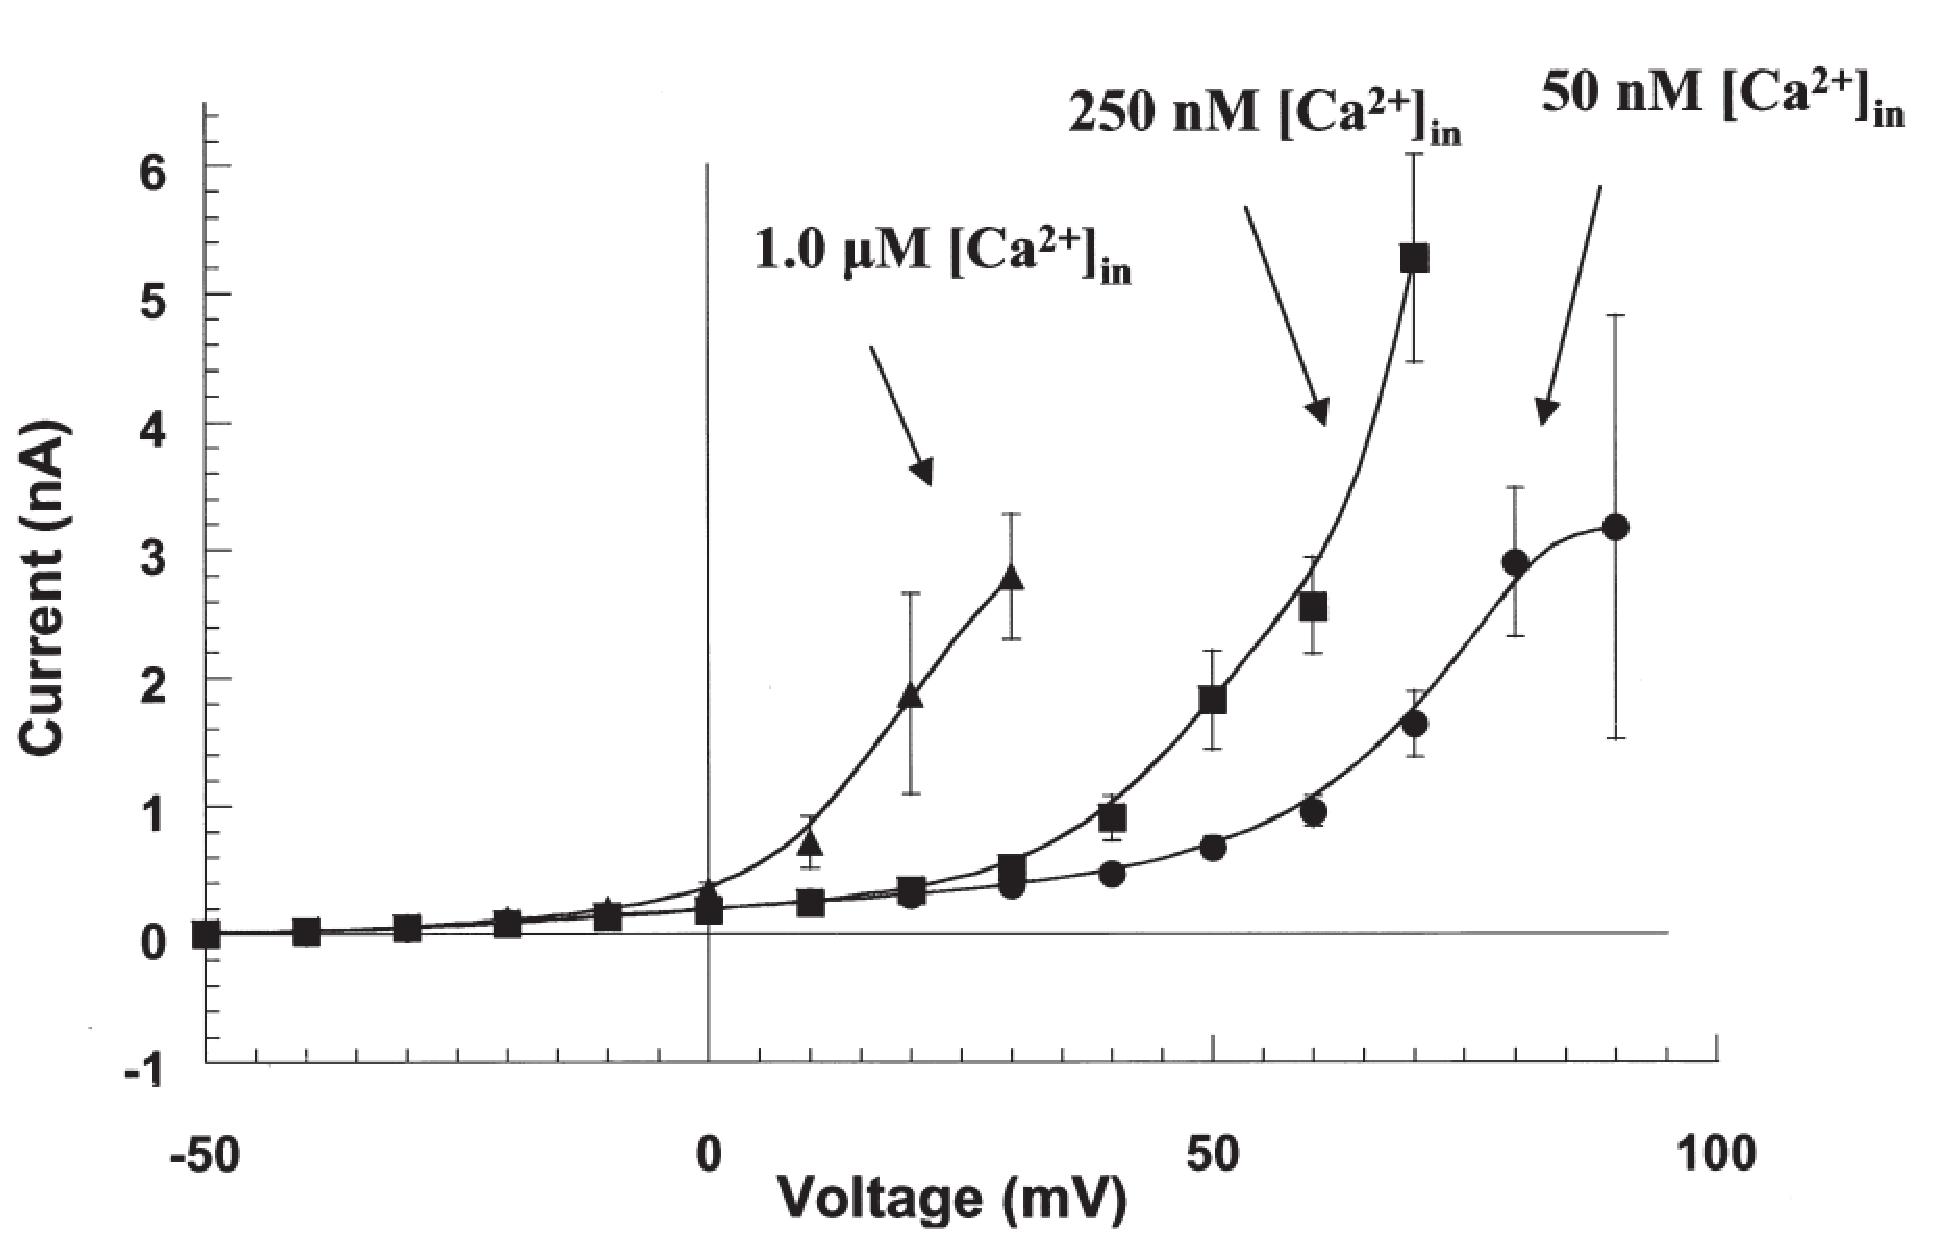
\includegraphics[height=5cm,
    angle=0]{./images/MaxiK_Vdependent.eps}}
  \caption{The I-V relationship for maxi-K channel current recorded at
  whole-cell level from human embryonic kidney cells \citep{gribkoff2001}}
\label{fig:MaxiK_Vm-dependent}
\end{figure}

\textcolor{red}{Inhibitors}: 37-aminoacid peptide charybdotoxin (ChTX) isolated
form venom of the scorpion is the first BK blocker with satisfactory of
selectivity. Other highly selective BK-blocker is Iberiotoxin (IbTX). Due to the
physiological role during the hyperpolarization process resulting from a $\K$
outflow, the channel is a potential drug target when using some compound to
activate the outward $\K$ current \citep{calderone2002}. Due to the large
conductance, BK channel is the promising candidate for drug target.
Another one is ATP-sensitive channels (K$_\ATP$).


\subsection{***** Type I: fast-activating, inactivating}

The channel develops rapidly (1-2 msec) and
decay within tens of miliseconds.

The inactivating BK channels Type I: ( $\alpha$ + $\beta$2).
$\beta$2 subunit confers N-type inactivation and  is sensitive to iberiotoxin
block. However, some splice products of $\beta$3 subunit also confer
inactivation; yet $\beta$3-expressed protein has weak expression in the brain
(Wallner et al., 1999; Xia et al., 1999; Uebele et al., 2000; Hu et al., 2003).

These channels are found in
\begin{enumerate}
  
  \item  CA1 (Cornu Ammonis-1) neurons of the hippocampus ( McLarnon, 1995 ) and
  
  \item adrenal chromaffin cells ( Solaro and Lingle, 1992 )
\end{enumerate}

GOAL: repolarize the first few, but not later, action potentials in a train,
resulting in a frequency-dependent spike broadening ( Shao et al., 1999; Faber
and Sah, 2003 ).



\subsection{***** Type I: fast-activating, non-inactivating}

non-inactivating type I: $\alpha$ alone, Fig.\ref{fig:BK(Ca)-type-I}.

This long-lasting outward current is blocked by a low concentration of TEA.
In neurons, BK channels colocalize with calcium  channels. It is also very
voltage-dependent at constant \ce{Ca^2+} concentration.
\footnote{http://elysium.wustl.edu/LingleLab/general.htm}.

\begin{figure}[hbt]
  \centerline{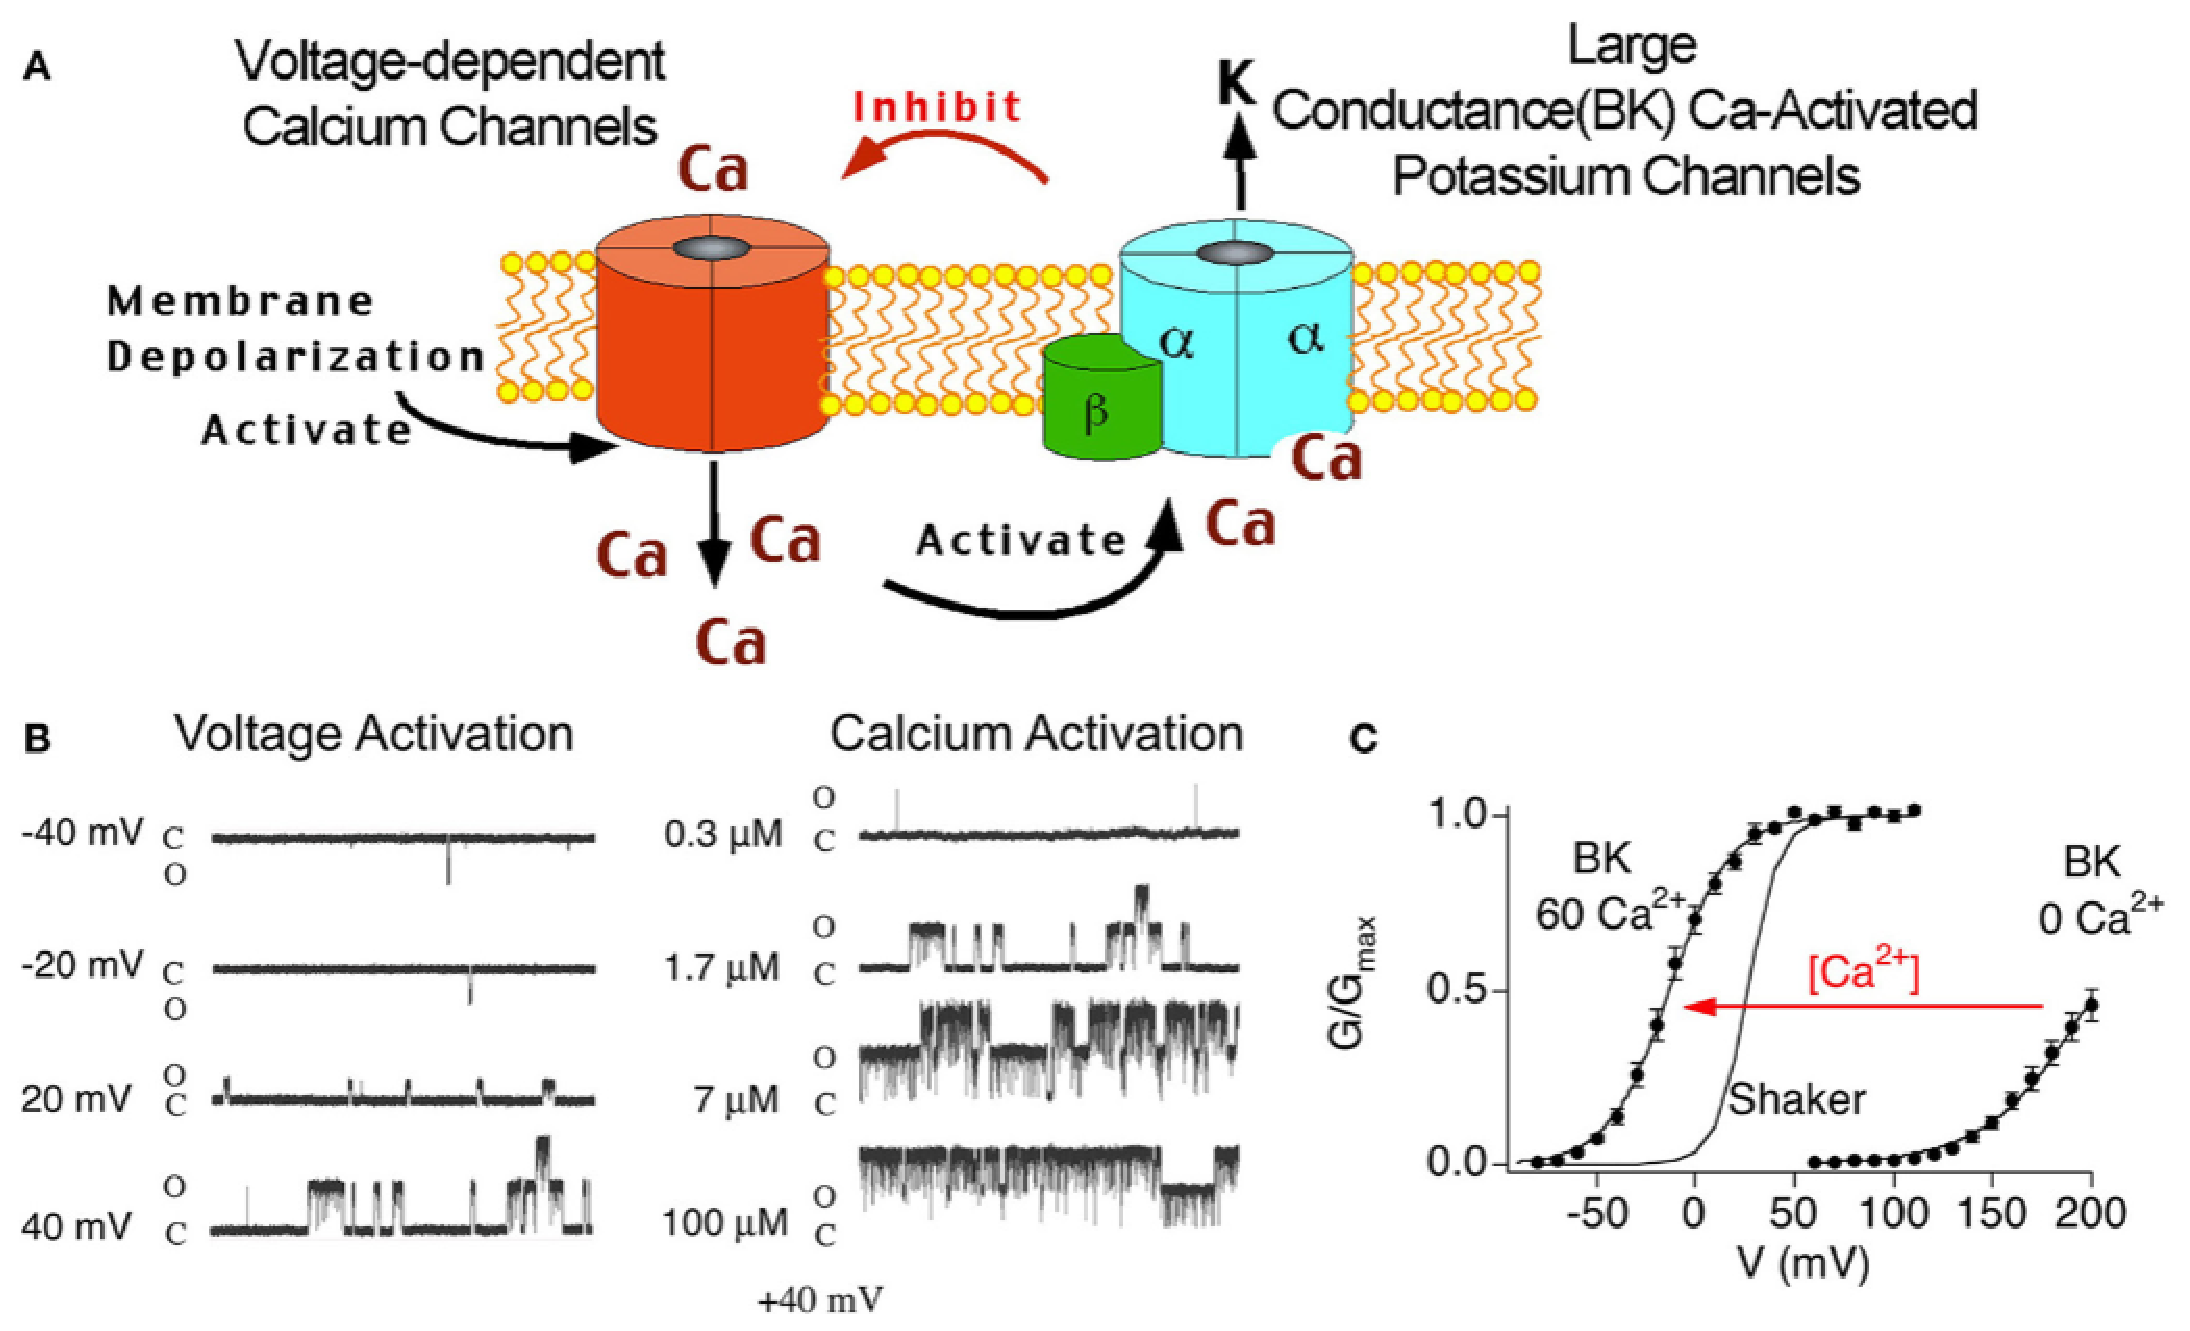
\includegraphics[height=3.4cm,
    angle=0]{./images/BK(Ca)-type-I.eps}}
\caption{BK(Ca) channel co-localize with $\Ca$ channels: (A) Depolarization
open $\Ca$ channel, the influx of $\Ca$ trigger BK(Ca), the opening of BK(Ca)
causes an outflux of $\K$ provides a negative feedback, i.e. in turns repolarize
the potential; (B) Single channel recording of BK(Ca) $\alpha$-alone: one at
various voltage, one hold voltage at +40mV, and test different $[\Ca]_i$; 
(C) conductance-voltage curve recorded from BK(Ca) $\alpha$-alone recorded from
inside-out patch (Sect.\ref{sec:patch_clamp-inside-out}): one with 0 $[\Ca]_i$
(using 5mM EGTA to buffer); and one with 60$\muM$ $[\Ca]_i$ }
\label{fig:BK(Ca)-type-I}
\end{figure}

\subsection{-- Type II BK(Ca): $\beta$4-containing BK(Ca) channel
(slow-activating, non-inactivating)}
\label{sec:BK(Ca)-type-II}

Type I subtype is sensitive to  scorpion venom (charybdotoxin and iberiotoxin).
However, the so-called "type II" subtype has the property of toxin resistance
and is slow-gated.

This unique property is due to the channel assembly with an accessory
neuron-enriched $\beta$4 subunit which not only occlude the toxin binding to BK
channel, but also slow the activation and deactivation kinetics(i.e.
$\alpha+\beta4$), Fig.\ref{fig:BK(Ca)-type-II}.
Until 2014, our understanding of the functional role of $\beta$4-containing BK
potassium channels in neurons is still very limited.

$\beta$4 modulates steady-state properties  (Behrens et al., 2000; Brenner et al.,
2000; Lippiat et al., 2003; Ha et al., 2004; Wang et al., 2006).
\begin{itemize}
  \item  by causing negative shifts of the conductance-voltage relations in high
  calcium ($[\Ca]_i > 10 \muM$)
  
  \item by causing positive shifts of the conductance-voltage relations in low
  calcium. Two proposed mechanisms
  \begin{enumerate}
    
    \item  $\beta$4, like the related $\beta$1and $\beta$2, cause an increased
    energetic barrier for gate opening ( Orio and Latorre, 2005; Wang and
    Brenner, 2006; Wang et al., 2006).
    
    \item reduce gating charge which also can contribute to reduced channel
    openings (Contreras et al., 2012)

  \end{enumerate}
\end{itemize}

\begin{figure}[hbt]
  \centerline{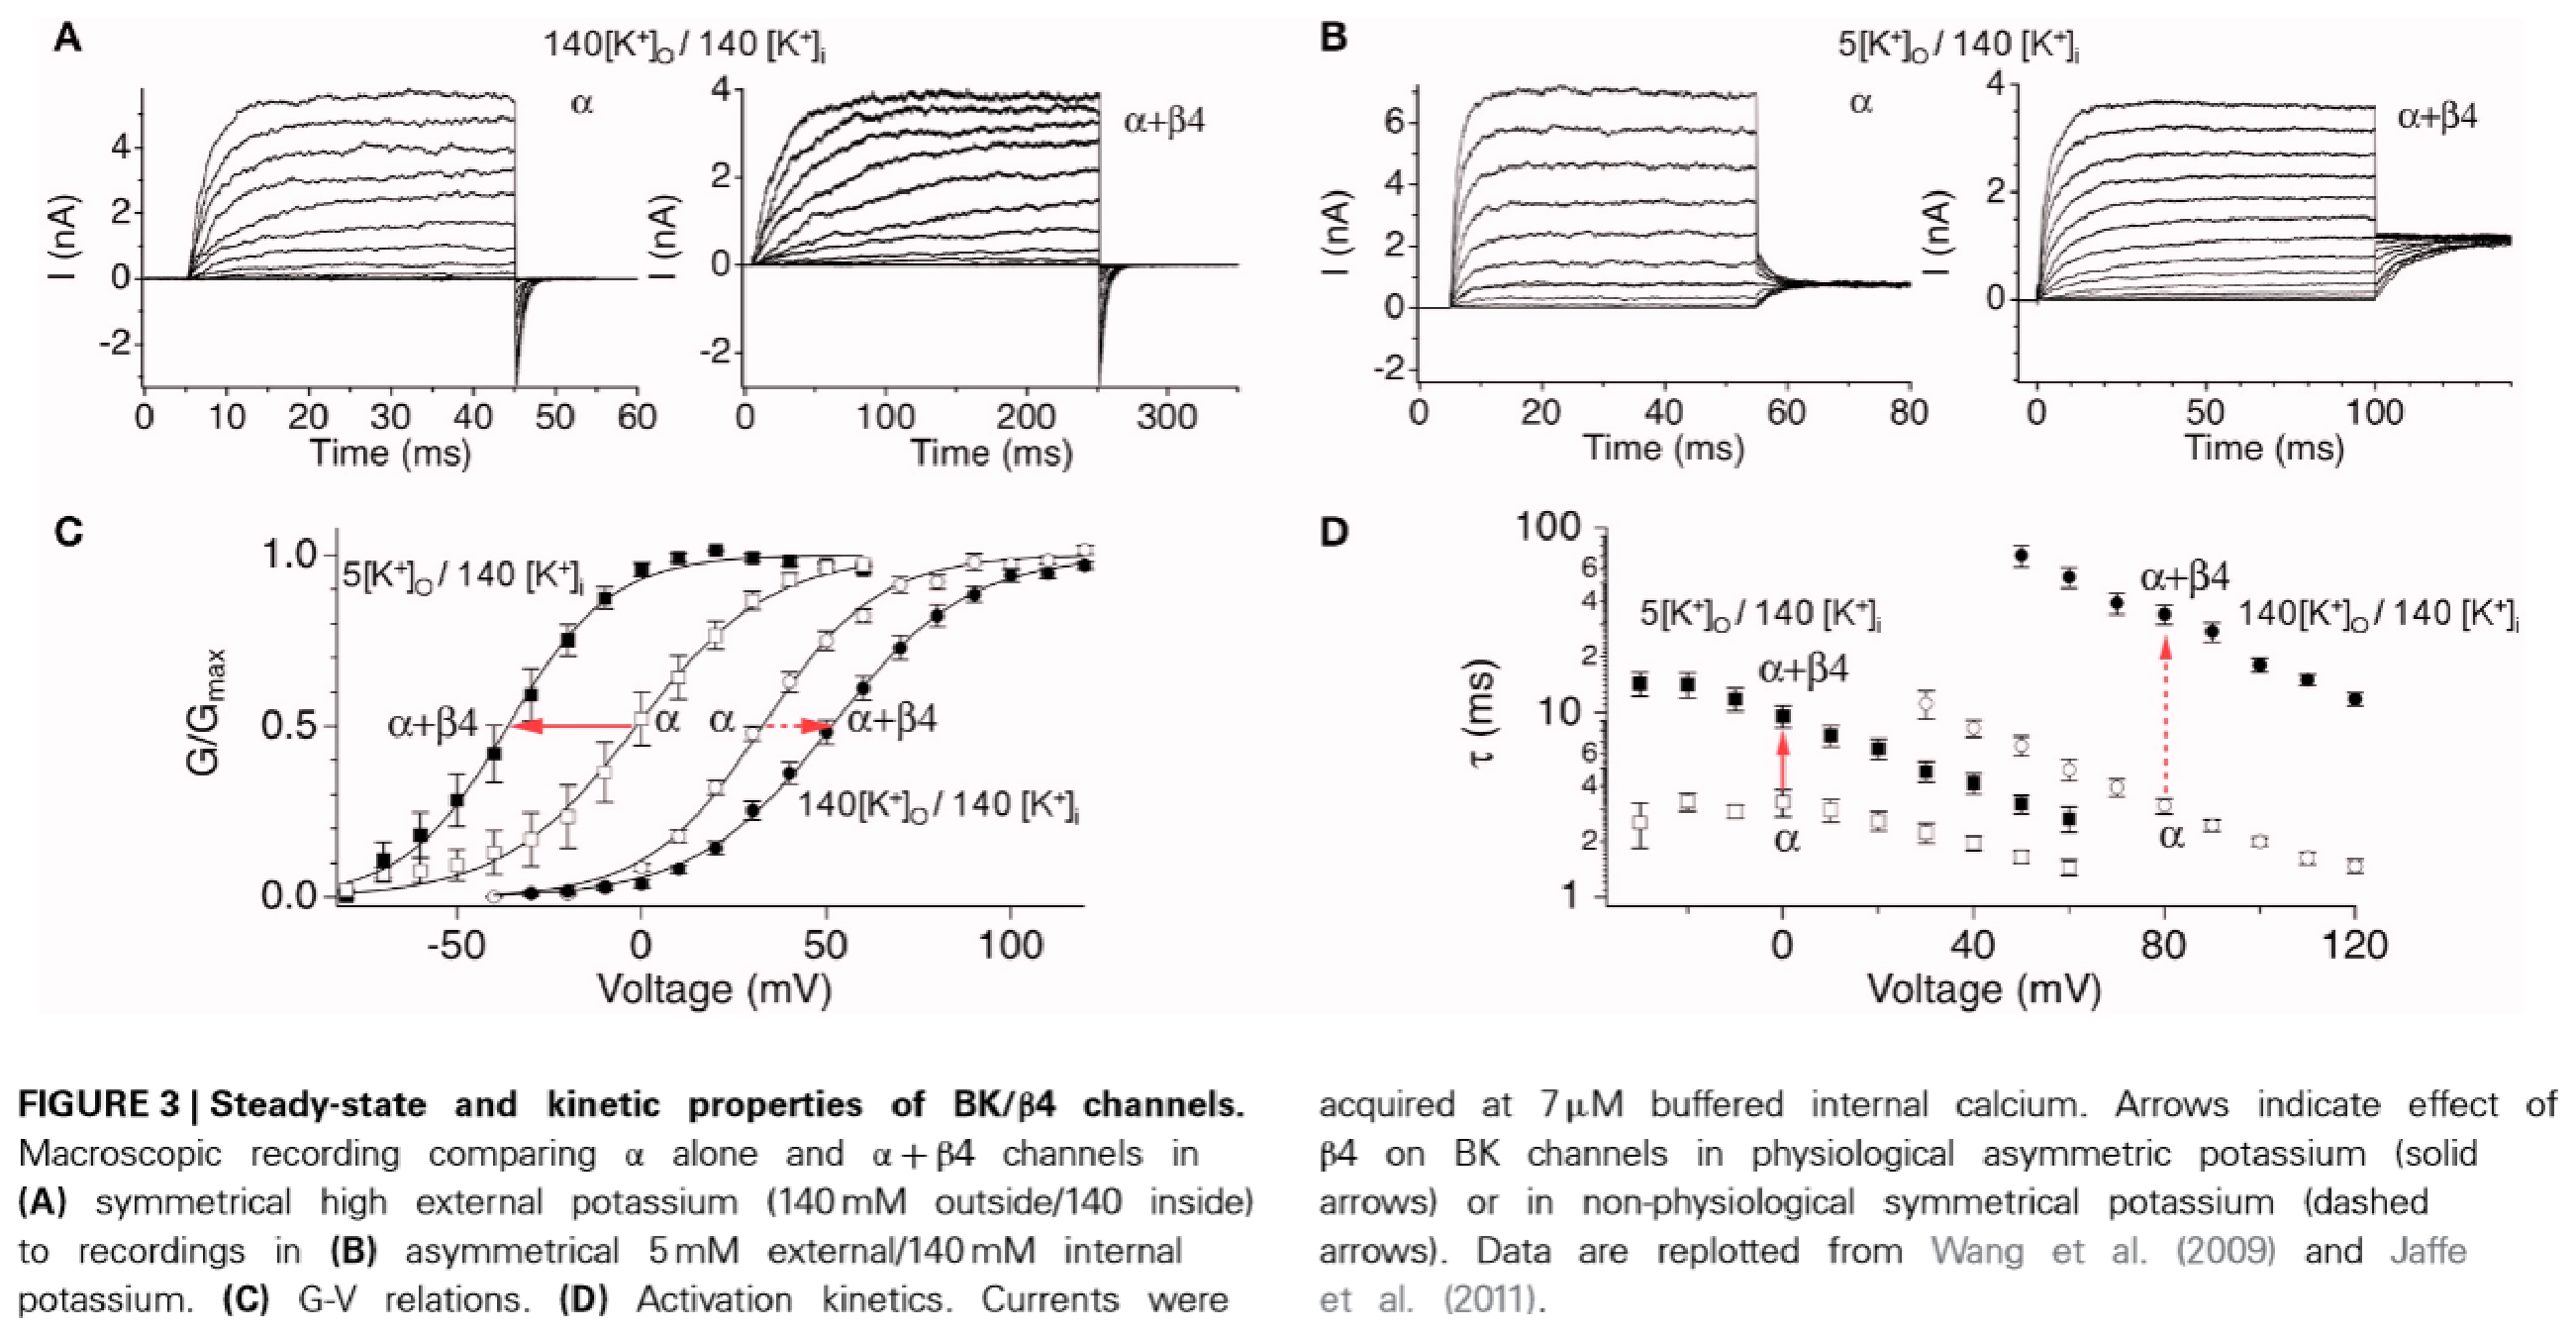
\includegraphics[height=6.4cm,
    angle=0]{./images/BK(Ca)-type-II.eps}}
\caption{BK(Ca) type II: (A) the widely used recording with symmetrical, high
potassium concentrations (replacing external sodium with potassium; 
(B)  at physiological external sodium, low external potassium
concentration instead indicate that $\beta$4 confers a negative shift of
the G-V relationship at all calcium concentration}
\label{fig:BK(Ca)-type-II}
\end{figure}

The channels are found in  \citep{wang2014}
\begin{enumerate}
  \item dentate gyrus granule neurons and in purkinje neurons of the cerebellum.

In these neurons, the role of these channels is largely consistent with
slow-gated channels that reduce excitability either through an interspike
conductance, such as in purkinje neurons, or by replacing fast-gating BK
channels that otherwise facilitate high frequency AP firing, such as in dentate
gyrus neurons. 

  \item More recent studies suggest that $\beta$4 subunits may also be
  expressed in some neurons lacking iberiotoxin-resistant BK channels, such as
 in CA3 hippocampus neurons.
\end{enumerate}

$\beta$4 dramatically promotes BK channel opening by shifting voltage sensor
activation to more negative voltage ranges, but also slows activation to
timescales that theoretically preclude BK ability to shape action potentials
(APs).

IMPORTANT: $\beta$4 surface membrane trafficking is regulated through an
endoplasmic reticulum (ER) retention signal and carboxyl-terminal
palmitoylation.

\subsection{SK current (KCa2.x current): small conductance (gated solely by
$[\Ca]_i$)}
\label{sec:SK_current}

NAMES: KCa2.1 (SK1, encoded by {\it KCNN1} gene in human), KCa2.2 (SK2, KCNN2),
KCa2.3 (SK3, KCNN3)
\begin{itemize}
  \item hSK1 (560 aa): human SK, or (due to the intermediate conductance) IK
  channel (Sect.\ref{sec:IK_current})

  \item rSk1 (Sect.\ref{sec:SK_current-2.1}): rat homologue of human SK1

  \item rSK2 (580 aa), rSK3 (553 aa):

\end{itemize}
These channels as classified based on either apamin-sensitive
(Sect.\ref{sec:SK_current-apamin-sensitive}) or apamin-insensitive
(Sect.\ref{sec:SK_current-apamin-insensitive}).
Many, but not all SK channels are blocked by apamin and the plant alkyloid,
$d$-tubocurare (dTC) (Kohler et al., 1996).
The molecular basis for this is due to two residues, an aspartic acid and an
asparagine, which reside on opposite sides of the deep pore and are essential
for apamin sensitivity.
Exchange of either one of the residues found in SK2 into the sequence of SKI
endows partial apamin sensitivity, while exchange of both residues renders SKI
channels as sensitive to apamin as SK2 channels.

A closely related channel encoding an intermediate-conductance calcium-activated
potassium channel (IK channel) with functional and pharmacological
characteristics consistent with the Gardos channel has been reported by several
groups (Sect.\ref{sec:IK_current}).


\begin{itemize}
  \item rSK2 is blocked by extracellular apamin at $K_i = 63$ pM.

NOTE: hSK1 is not affected even at 100 nM apamin.
  
  \item rSK2 is blocked by extracellular dTC at $K_i = 2.4\muM$
  
NOTE: hSK1 is 30-fold less sensitive to dTC, i.e. $K_i = 76.2\muM$
   
\end{itemize}


Small-conductance Ca-activated K channels ({\bf SK K(Ca)}) are potassium
selective and are activated by an increase in the level of intracellular
calcium,  such  as  occurs  during  an  action  potential.
 SK channels is responsible for
slow, long lasting afterhyperpolarization (sAHP -
Sect.\ref{sec:AHP-slow}) in neurons that follows the spike and modulate
firing frequency; thus giving it the name $I_{\AHP,d}$.
The channels varies considerably in different cell types, activating slowly (10
to 1000 ms), and it may decay over several seconds.
Their  activation  causes  membrane hyperpolarization, which inhibits cell
firing and limits the firing frequency of repete tive  action  potentials.

The channel is activated by Ca2+ entering either directly through voltage-gated
Ca2+ channels, or through Ca2+-induced Ca2+ release, depending on the neuronal
subtype.
The decline in $I_\AHP$ can be more closely related to $\Ca$ diffusion from the
membrane.  However, several studies have pointed to a mismatch between the fast
kinetics of intracellular Ca2+ and the slow activation of sIAHP, and various
theories have been proposed to explain this phenomenon.

Ca2+ gating of the SK channels is accomplished by constitutive association of
calmodulin (CaM) with the intracellular COOH-terminal domain of the channel
$\alpha$-subunits called the CaM binding domain (CaMBD). Apart from gating, CaM
is also required for channel assembly and trafficking.

Ca-activated K channels play important functional roles in regulating {\bf
firing frequency} (\ce{Ca^2+} accumulate upon repetitive firing, spike frequency
adaptation), cell's metabolism (e.g. provide a negative feedback to regulate
\ce{Ca^2+} entry).  If Ca entry takes place during AP, the slow AHP K(Ca) are
responsible for AHP that follow the spike and play major role in modulating {\it
firing frequency}.

\begin{mdframed}

Betweek SK1, SK2 and SK3, the intracellular N- and C-termini of the different
subunits lack the homology seen among the other domains, suggesting that they
may endow functional specificity such as regulation by second messengers.

\end{mdframed}

\subsection{** Apamin-sensitive}
\label{sec:SK_current-apamin-sensitive}

SK2 (Sect.\ref{sec:SK_current-2.2}) and SK3 (Sect.\ref{sec:SK_current-2.3}) are
apamin sensitive. The voltage-independent, Ca2+-dependent small K current (SK
current), with single channel conductance about 10-14pS (or 5-20pS in symmetrical 120mM
potassium on both sides of the membrane (Bond et al., 1999), is
apamin-sensitive.
\begin{enumerate}
  \item  SK channel activates at very low 0.01-0.1$\muM$ of $[\Ca]$, with little
  or no $V_m$-dependent.

  \item When [\ce{Ca^2+}] is lowered from 2 to 0.2 mM, then {\it slow AHP} is
disappeared; only {\it fast AHP} remains (Sect.\ref{sec:BK-current}). 
\end{enumerate}

There are at least 3 different genes encode the channels, giving 3 subtypes of
SK channels: Sect.\ref{sec:SK_current-2.1}, Sect.\ref{sec:SK_current-2.2} and
Sect.\ref{sec:SK_current-2.3}.
Each subtype of SK channels consists of a pore-forming $\alpha$-subunit of 6 TMs
that is about 550-730 amino acids in length with its intracellular COOH and NH2
termini. Many data suggested calcium  ions  do  not  interact directly with the
SK channel $\alpha$ subunit; but indirectly through the constitutive interaction
with calmodulin and subsequent calcium-dependent conformation alterations.

\begin{itemize}
  \item  Three different isoforms of SK channels were found in heart and the
  differential expression of SK1 and SK2 in mouse atria and ventricles (Tuteja et al. 2005). 
  
  \item Voltage-independent, apamin-sensitive K+ channels activated by
  submicromolar concentrations of Ca2+ (with half-activation $K_{1/2}=0.3 \muM$
  and Hill coefficient $\eta$ close to 4) have been described for peripheral
  cell types, inclUding skeletal muscle, gland cells, and T lymphocytes.
\begin{equation}
g_\SK = \bar{g_\max}\frac{1}{1 + \left(\frac{K_{1/2}}{[\Ca]} \right)^\eta}
\end{equation}   
\end{itemize}

The physiological kinetics of K(Ca) channels in different cells would be a
complex blend of kinetics of \ce{Ca^2+} entry, \ce{Ca^2+} buffering and
diffusion, \ce{Ca^2+} uptake and extrusion into intracellular organelles,
\ce{Ca^2+} binding to the channels, and voltage-dependent transitions.
%  Experimental results shown that SK K(Ca) channels make {\it slow AHP} (afer
% hyperpolarization).



\begin{mdframed}

BK(Ca) current is voltage-dependent and tends to turn-off at voltage
closed to resting potential (-70mV to -60mV) at physiological concentration of
\ce{Ca^2+}. 

The turn-off of $I_{AHP}$, on the other hands, may be more closely to the
diffusion of $\Ca$ away from the membrane (i.e. need submembrane compartment).
\end{mdframed}

Apamin-sensitive SK channels (SK2, SK3) have been implicated in several
important physiological processes such as excitability, sleep-wake cycles,
learning and memory, and digestive system activity. A provocative study suggests
that the SK3 gene may be linked to some forms of bipolar disorder.
Denervated skeletal muscle, or skeletal muscle from patients with myotonic dystrophy
(DM49) contains apamin-sensitive SK channels and radiolabeled apamin binding sites,
while normal adult skeletal muscle does not. These results suggest SK channels may
be valuable targets for therapeutic intervention (Bond et al., 1999).

\subsection{-- SK2: KCa2.2}
\label{sec:SK_current-2.2}

SK2 and SK3 are apamin sensitive (Sect.\ref{sec:SK_current-apamin-sensitive}).
SK2 has IC50 as 60 pM (Bond et al., 1999).
Single SK2 channel activity is dependent upon calcium and is quantitatively
similar to macroscopic currents.

Analysis of stationary SK2 channel behavior showed two modes of gating: low Po
and high Po.
\begin{itemize}
  \item  
  when $1\muM$ $\Ca$ is applied to single channel patches, the Po is 0.6; but
  also a low Po of 0.05 is also observed. Channels switch spontaneously and
  rapidly between the two modes
  
  \item the frequency of mode switches and time spent on each mode is $\Ca$
  dependent.
\end{itemize}
The two modes share many features, having similar open times and short and
intermediate closed times.
However, the long calcium-dependent closed time in the low open probability mode
is much longer - several hundred milliseconds to seconds - than the long closed
time in the high open probability mode.

SK channel gating may be modeled by a scheme with four closed and two open
states, which reproduces very well the single-channel data.

\subsection{-- SK3: KCa2.3}
\label{sec:SK_current-2.3}

SK2 and SK3 are apamin sensitive (Sect.\ref{sec:SK_current-apamin-sensitive}).
SK3 has IC50 as 1 nM.
SK3 channels, which have an intermediate sensitivity to apamin, contain one of
the two determinant residues for apamin sensitivity, consistent with the
mutagenesis studies.

SK3 showed similar levels of expression in atria and ventricles.





\subsection{** Apamin-insensitive SK (hSK1)}
\label{sec:SK_current-apamin-insensitive}

Apamnin-insensitive SK channels have also been reported such hSK1 (in human) -
Sect.\ref{sec:IK_current}. If we look at apamin-insensitive sAHP, the kinetics
is quite different from that of apamin-sensitive sAHP (Sect.\ref{sec:AHP-slow}).


\subsection{-- SK1: KCa2.1}
\label{sec:SK_current-2.1}

SKI is not blocked by apamin (100 nM).
SK1 is expressed in regions that have apamin-insensitive sAHPs, such as
hippocampal pyramidal neurons (Sect.\ref{sec:AHP-slow}).
SK1 transcript was found to be more abundant in atria compared with ventricles,
similar to the previously reported finding for SK2 channel.

Variants of mouse SK1 channel (mSK1) differ mainly in the COOH-terminal
structure, affecting a portion of the sixth transmembrane segment (S6) and the
calmodulin binding domain (CaMBD).


\subsection{-- IK current (KCa3.1): intermediate conductance}
\label{sec:IK_current}

NAMES: KCa3.1 (IKCa1, SK4, KCNN4)

IK channel is a closely related channel to SK channels, encoding an
intermediate-conductance calcium-activated potassium channel with functional and
pharmacological characteristics consistent with the Gardos channel The IK
channel has a similar properties as SK1 current (Sect.\ref{sec:SK_current-2.1},
i.e. apamin-insensitive, a Calmodulin-mediated $\Ca$-dependent activation; yet
it has a higher conductance: 20-85pS.


There is only one gene (hKCa4 from  human T lymphocytes, hIK1 from human
pancreas) found encoded for the  intermediate conductance calcium-activated
potassium channel (IK) channel \citep{ishii1997, logdson1997}.
The gene from human is KCNN4, with 6 transmembrane domain (S1-S6), with 41-42\%
similarity in sequence with 3 genes encoded for SK channels
(Sect.\ref{sec:SK_current}). 
\begin{enumerate}

  \item hIK1 gave rise to inwardly rectifying potassium current in Xenopus
  oocyte (activated by $[\Ca]_i$ at $K_{0.5} = 0.3 \muM$), with the slope in
  Hill equation is 1.7 and single-channel conductance of 39 pS in the inward
  direction.
  
   hIK1 currents were reversibly blocked by charybdotoxin (Ki = 2.5 nM) and
  clotrimazole (Ki = 24.8 nM) but were minimally affected by apamin (100 nM),
  iberiotoxin (50 nM), or ketoconazole (10 $\muM$),
  
  \item 
\end{enumerate}
The channel is potentially blocked by scorpion toxin charybdotoxin (ChTx) and the antimycotic
clotrimazole (CLT). So, the role of IK channels as a potential drug target has
also been examined \citep{jensen2001, jensen2002}.


Expression:
\begin{enumerate}
  \item express in human lung mast cell (HLMC):
it plays a critical role in the cell's migration to diverse chemotactic stimuli,
and to a lesser extent in their degranulation. Drugs that directly block this
channel or which close it indirectly therefore have potential as
novel therapies for mast cell-dependent disease.

The activation of KCa3.1 is attenuated, i.e. the channel is closed, by albutamol
and adenosine via $\beta-$adrenoreceptor
(Sect.\ref{sec:beta-adrenergic-receptor}) and adenosine A2A receptor
(Sect.\ref{sec:A2A-receptor}) through Gs-coupled mechanism independent of cAMP.
It is later confirmed that the activation of EP2 receptor would also close
KCa3.1 (Duffy et al., 2008).
% http://onlinelibrary.wiley.com/doi/10.1002/eji.200738106/pdf

\label{ref:GPE2}
Prostaglandin E2 (PGE2) is a prostanoid with four specific GPCR, i.e.
EP1, EP2, EP3 and EP4.
\begin{itemize}
  \item EP4 coupled to Gs
  \item EP3 coupled (predominantly) to Gi; and lesser to Gs.
  
PGE2 promotes degranulation and migration of mouse bone marrow-derived mast
cells through the Gi-coupled EP3 prostanoid receptor, and induces LTC4 and
cytokine secretion from human cord blood- derived mast cells.

  \item EP2 coupled to Gs

PGE 2 binding to the Gs-coupled EP 2 receptor on HLMC inhibits their
degranulation (in opposite to EP3)

  \item EP1 receptors mobilize $[\Ca]_i$, probably through Gq.
\end{itemize}
mouse mast cells express the EP3 receptor whose activation induces both
degranulation and chemotaxis.

Human cord blood-derived mast cells, express both EP2 and EP3 receptors.

  
  \item 
\end{enumerate}


\subsection{---- Gardos channel}
\label{sec:Gardos-channel}

The first demonstration that internal calcium ions regulate potassium flux was
provided by Gardos from red blood cells.
The electrophysiological and pharmacological properties of the Gardos channel
show that it belongs to the IK subfamily (Sect.\ref{sec:IK_current}). 
\begin{itemize}
  \item 50 pS at -120 mV
  \item 13 pS at 120 mV
\end{itemize}

It is blocked by charybdotoxin (CTX) but not the structurally related peptide
iberiotoxin (IBX), both of which block BK channels.

\subsection{K(Ca) agonists/antagonists}
\label{sec:K(Ca)_agonists}
\label{sec:K(Ca)_antagonists}

{\bf Antagonists}
\begin{enumerate}
  \item Charybdotoxin (CTX): block small- and medium-conductance K(Ca)
  channels - Sect.\ref{sec:MaxiK-current} [Garcia et al., 1995]
%Charybdotoxin and its effects on potassium channels.  


  \item iberiotoxin (ibTX):block maxi-K(Ca) or BK(Ca) with high affinity Kd
  $\approx$ 1 nM by decrease both probability of opening, and the open time as
  well.
  
  \item agitoxin 2 (AgTX2)
\end{enumerate}
%\section{Inward-rectifier}


\section{AHP currents: $I_\AHP$, sI$_\AHP$}
\label{sec:AHP-currents}


After hyperpolarization (Sect.\ref{sec:ahp-after-hyperp}) refers to the
prolonged depolarization after an action potential. This is the result of one or
many outward $\K$ currents; collectively denoted as $I_\AHP$.

As the AHP can be divided into slow AHP (sAHP) and fast AHP (fAHP) -
Sect.\ref{sec:AHP-slow}  and Sect.\ref{sec:AHP-fast}, the $I_\AHP$ can be the
result of
\begin{enumerate}
  \item Myenteric neurons of guinea-pig ileum:
  
  Charybdotoxin and iberiotoxin sensitive K+ channels, i.e.
  opening of a large-conductance (BK) calcium-dependent potassium channel.
  There is no apamin-sensitive K+ channels involved [Kunze et al., 1994]. 
  %Kunze WA1, Bornstein JC, Furness JB, Hendriks R, Stephenson DS.
  %Charybdotoxin and iberiotoxin but not apamin abolish the slow
  % after-hyperpolarization in myenteric plexus neurons.
  
  \item 
\end{enumerate}

\section{$I_\to$}
\label{sec:Ito1}
\label{sec:Ito2}  
\label{sec:Ito-current}

% $I_{\to,1}$ and $I_{\to,2}$
In cardiac myocytes, there are two components of transient
  outward fast-inactivating potassium current $I_\to$ :
\begin{enumerate}
  \item 
  a larger, voltage-activated (rapidly activating and inactivating),
  4-AP-sensitive $I_{\to,1}$; and
  
  \item a smaller, calcium-activated $I_{\to,2}$. 
\end{enumerate}
In many cases, different authors use  $I_{\to}$ as referring to $I_{\to,1}$.
  
  
  In atria, Purkinje fibers and subepicardial ventricular cells, the current
  denoted as transient outward K + current $I_\to$, gives the typical
  ``spike-and-dome" appearance (the notch).


\subsection{--  $I_\tof$, HERG channel}
\label{sec:Itof_channel}
\label{sec:HERG_channel}

In cardiac cell, the current is used interchangbly with the notation $I_\Kr$
(Sect.\ref{sec:IKr_current}), as HERG channel ($I_\Kr$): HERG gene in {\it
Xenopus} oocytes induces a current with properties similar to $I_\Kr$
(Sect.\ref{sec:IKr_current}) \citep{sanguinetti1995, trudeau1995}.

The gene hERG (human-Ether-a-go-go-Related Gene) is the human homolog of the
gene found in Drosophila called Ether-a-go-go gene (the gene when aneasthetised
with Either, the leg start shake, like the porpular dancing at the Whisky A
Go-Go night club in West Hollywood, CA - (Sect.\ref{sec:Eag-like_Kchannel})).
The superfamily that includes this channel is the Shaker family as the
channel was first cloned in a mutant of the fruit fly {\it Drosophila}
(Sect.\ref{sec:Shaker-gene}). 
In human, the gene is called HERG (human ether-\'a-go-go-related gene). When
HERG is mutated, it give an abnormal Kr current that explains one type of
long QT syndrome.

The encoded channel play an important role in regulating heart's beat, by
mediating the underlying $I_\Kr$ current in cardiac
AP~\citep{mazhari2001,clancy2001,oehmen2002,fink2008}. The loss of functionality
in channels' conductance may result a potentially fatal disorder called {\bf
long QT syndromes}; while the gain of functionality may result into {\bf short
QT syndrome}. Both disorders can lead to the risk of lethal cardiac arrhythmias,
due to repolarization disturbances in the cardiac AP. There are more mutations
that lead to long QT syndrome than for shrot QT syndrome
\citep{hedley2009}

\subsection{-- $I_\tos$}
\label{sec:Itos}

\section{KQT-like potassium channels (C. elegans)}
\label{sec:KQT-like-K+-channel}

In {\it C. elegans}, KQT potassium channels are related to the human KvLQT
(KCNQ) channel family (Sect.\ref{sec:KCNQ}).  C. elegans has three genes
encoding channels of the KQT family.

In humans, there are five of these genes in humans (KCNQ1-5).
Remarkably, four of the five human genes are associated with hereditary
diseases. In addition to long-QT syndrome (associated with KCNQ1), KCNQ
mutations have been linked with Benign Familial Neonatal Convulsions (KCNQ2 and
KCNQ3; Biervert et al., 1998; Charlier et al., 1998; Singh et al., 1998 and
2003), and the Non-syndromic Autosomal Deafness, DFNA2 (KCNQ4; Kubisch et al.,
1999).

KQT1 in C.elegans is the homologue to KvLTQ1 in humans.

\section{Eag-like potassium channels}
\label{sec:Eag-like_Kchannel}
\label{sec:erg-related-gene}

Eag-like channels (Ether-a-go-go) refers to channel encoded by the Drosophila
ether-a-go-go (eag) gene. 

 Eag-like channels form a diverse family in {\it C. elegans}
\begin{itemize}
  \item Eag
  \item Erg (Eag-related gene)
  
Although they are voltage-gated K+ channels constructed of subunits with six
transmembrane domains, functionally, erg channels are inward rectifiers. This
inward rectification is due to fast inactivation kinetics combined with slow
activation as well as fast recovery from inactivation combined with slow
deactivation.

  
  \item Elk
\end{itemize}

The human orthologue is {\it Herg}-like channel (Sect.\ref{sec:HERG_channel})
which encoded by HERG gene whose mutations can cause long QT syndrome type 2
(LQT2).



\section{Kinetics}

K channels vary widely in kinetics, voltage-dependent, single-channel behaviors,
etc, Fig.\ref{fig:KA-current-Kdr-current}. A review of K channels is given by
Rudy~\citep{rudy1988duk}.

\begin{figure}[hbt]
  \centerline{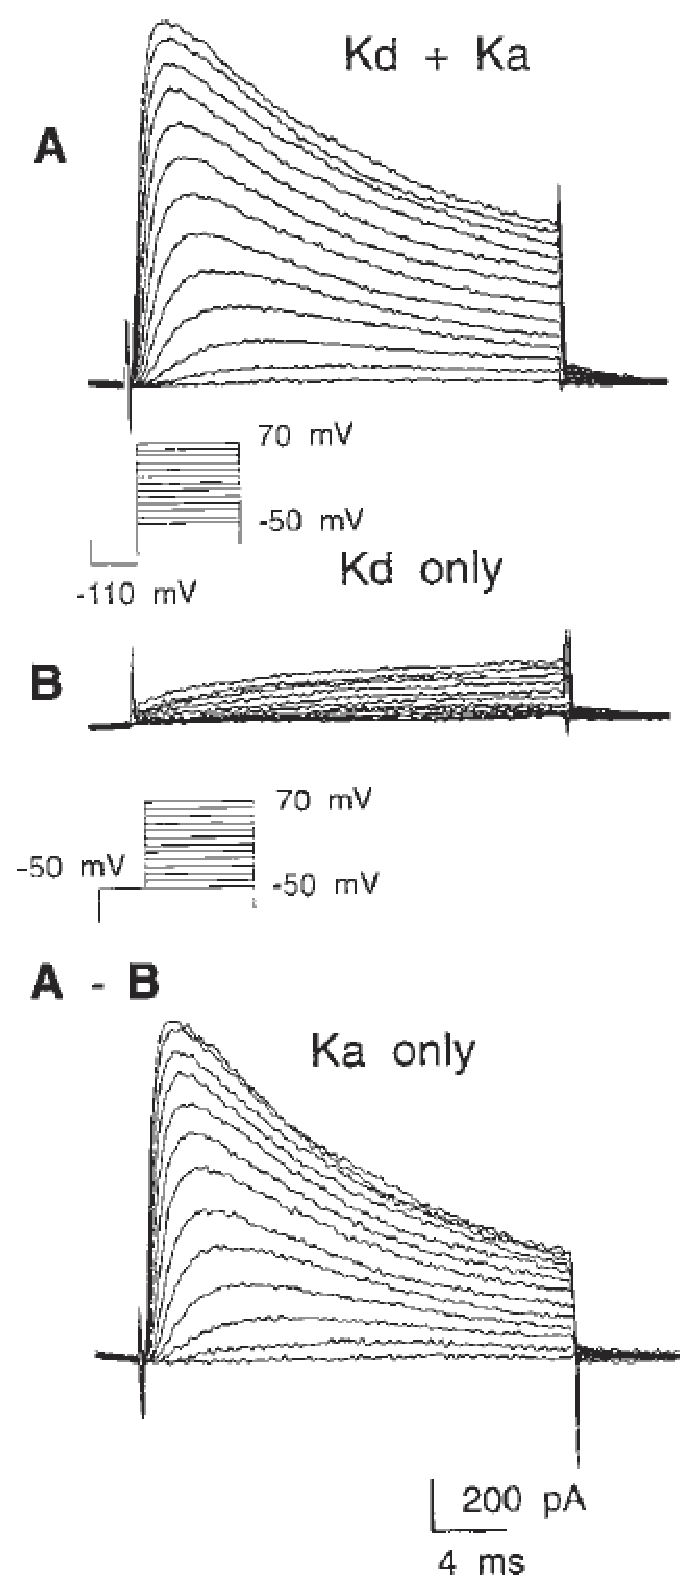
\includegraphics[height=6cm,
    angle=0]{./images/KA-current-Kdr-current.eps}}
  \caption{(A) Kdr (delayed-rectifier K+) + KA ('A'-type K+) recordings from
a spinal-cord astrocyte activated from holding potential -110 mV (step protocol
see inset); (B) same cell and same voltage-step
protocol but steps originated from a different holding potential -50mV (which
blocks KA current); (C) KA current is found by subtracting (B) from (A)}
\label{fig:KA-current-Kdr-current}
\end{figure}


Experimental studies have shown the many types of $\K$ channels, with many of
thems are present in almost every eukaryotic cells. However, they are different
in many ways, e.g. voltage-dependency, pharmacology, single-channel conductance
and other properties. \ce{K+} channels play critical roles in defining action
potential frequency and duration (in cardiac cells), and repetitive firing
properties (in nerve cells). Dysfunctions of particular \ce{K+} channels have
been implicated in epilepsy, ataxias, and various cardiac arrhythmias.

At normal condition, the concentration of $[\K]$ is much higher inside vs.
extracellular. This outward gradient makes the $\K$ to move outward easier than
inward. The early discovered $\K$ channel is the outward transient $\K$ current.
% To produce the depolarizing signals, the inward current via $\Na$ channels
% and/or $\Ca$ channels needs to overcome the outward \ce{K+} channels.
As a matter of fact, when $\K$ current was first incorporated into an
electrophysiological model by \citep{hodgkin1952ap} for the squid giant axon,
this current was shown to be responsible for the repolarization of the AP, and
was called outward delayed rectifier $I_\Kdr$. The onset of AP is the result of
the inward of $\Na$ and/or $\Ca$ across the sarcolemma. The repolarization of
$V_m$ required the extrusion of ions, which is controlled by 3 types of $\K$
channels, Fig.\ref{fig:Kcurrent_all} \citep{sanguinetti1997}.

However, due to the complexity in $\K$ current as we mentioned earlier, there is
inward $\K$ current as well. The inward rectifier $\K$ current discovered later
was then given the name {\it anomalous current}. Now, we introduce the role of
different types of $\K$ channels during an AP.
The APD in nerve and skeletal cells is short, while it's longer in cardiac
ventricular myocytes (several hundred of milliseconds), depending on species and
depending on the regions (endo- side or epi-side) on the ventricular wall.
This prolonged (plateau) phase is essential for normal EC-coupling in the heart.
This long AP is the result of many types of $\K$ channels either activate
slowly, inactivate rapidly, or conduct less current at positive potentials. This
leads to the net effect in that the outward current is small soon after the
initiation but incomplete phase of repolarization.


\section{In Neurons}

There are different voltage-gated potassium channels residing on central
neurons. However, it is more important to focus on potassium channels on
dendritic spines - neuronal locus of plasticity, where short-term alterations in
synaptic strength are assumed to be converted to long-lasting memories that are
embedded in stable morphological changes.

Previous studies revealed the expression of the voltagegated K+ channel subunits
Kv$\alpha$1.2, Kv$\alpha$1.4 Kv$\alpha$2.1, Kv$\beta$1.1 and Kv$\beta$2.1 in L5
neocortical pyramidal neurones (Sheng et al. 1994; Rhodes et al. 1995, 1996).
Also, Kv$\alpha$4.2 and Kv$\alpha$4.3 subunits were detected in L5 neocortical
pyramidal neurones (Tsaur et al. 1997; Serodio \& Rudy, 1998). This suggested a
$\K$ channel is a heteroners, containing probably both $\alpha$ and $\beta$
subunits.

Dendritic spines: \citep{sala2014}
\begin{enumerate}
  \item Kv4.2 channels - carries transient $I_A$ current (Sect.\ref{sec:A-type-K+current})
  
  Distribution: distribute evenly on dendrites and spines, but with no
  preference to remote dendrites

 Factors: It was filamin doubles the
current density generated through the Kv4.2 channels in transfected
cell lines. However, a recent mapping study could not
localize filamin within dendritic spines of cultured hippocampal
neurons.
 
  \item voltage-independent/calcium-dependent potassium SK2 (small potassium)
  channels - 
  
  Distribution: resides at high concentrations
near postsynaptic density within dendritic spines
  
  Factor: it is activated by a rise in intracellular calcium, is
selectively blocked by apamin. Blockade of SK channels or their genetic deletion
increases excitability of dendrites and spines and enhances their ability to
undergo LTP. This channel is subject to modulation by the M1 muscarinic receptor
(reduces the sensitivity of this channel to intracellular calcium concentration,
increase in the size of the excitatory postsynaptic potential (EPSP), and may
underlie the effects of muscarinic drugs on learning and memory). Interestingly,
the channel is activated by an influx of calcium through the NMDA receptor

In the process of LTP, SK2 channel is assumed to be removed
from the plasma membrane, and thus increase excitability of
the dendritic spine

   \item GIRK: voltage-insensitive potassium channel assumed to be
selectively associated with the postsynaptic density is the G
protein-coupled K channel.

It complexes with protein kinase A, protein kinase C and phospholipase C, as
well as protein phosphatase 1, protein phosphatase 2A, and regulators of G
protein signaling, all of which modulate its activity.

It is assumed to be activated by the metabotropic
GABA receptor (GABA-B) and by serotonin to hyperpolarize
the spine membrane and cause depotentiation of the excitatory
synapse. Interestingly, morphine enhances GIRK channel
activity in the hippocampus.

While GIRK channels are not assumed to selectively localize in dendritic spines,
their interactions with excitatory neurotransmission has important implications
for dendritic spine plasticity.
\end{enumerate}

\section{In cardiac}

The cardiac inward-rectifier $\K$ channels (2TM-1P subunits) regulate the
resting membrane potential, the frequency of pacemaker cells and the shape and
duration of the cardiac action potential \citep{tamargo2004}.

For voltage-gated potassium currents (6TM-1P subunits), cardiac cells typically
display at least one transient outward current and several delayed rectifiers to
control the duration of the action potential. The molecular basis for each of
these currents is formed by subunits that belong to different Kvx.y subfamilies
and alternative splicing can contribute further to the diversity in native
cells.

Additional subunits have evolved by concatenation of two 2Tm-1P subunits
(4Tm-2P); dimers of such subunits yield voltage-independent leak channels.

A special class of 6TM-1P subunits encodes the 'funny' pacemaker current which
activates upon hyperpolarization and carries both Na and K ions.

\begin{enumerate}
  \item $V_m$-gated $\K$ channels: 
  \begin{itemize}
    \item rapidly-activating and inactivating transient outward current
    $I_{\to1}$
    \item ultrarapid $I_\Kur$
    \item rapid $I_\Kr$ and slow $I_\Ks$ components of the delayed rectifier
    current
    \item inward rectifier $I_{\k,1}$
  \end{itemize}
  
  \item ligand-gated $\K$ channels:
  \begin{itemize}
    \item adenosine triphosphate-sensitive $I_\KATP$
    \item acetylcholine-activated $I_\KAch$
  \end{itemize}
  
  \item 
\end{enumerate}

Changes in the expression of K+ channels explain the regional variations in the
morphology and duration of the cardiac action potential among different cardiac
regions and are influenced by heart rate, intracellular signalling pathways,
drugs and cardiovascular disorders.

\begin{figure}[hbt]
  \centerline{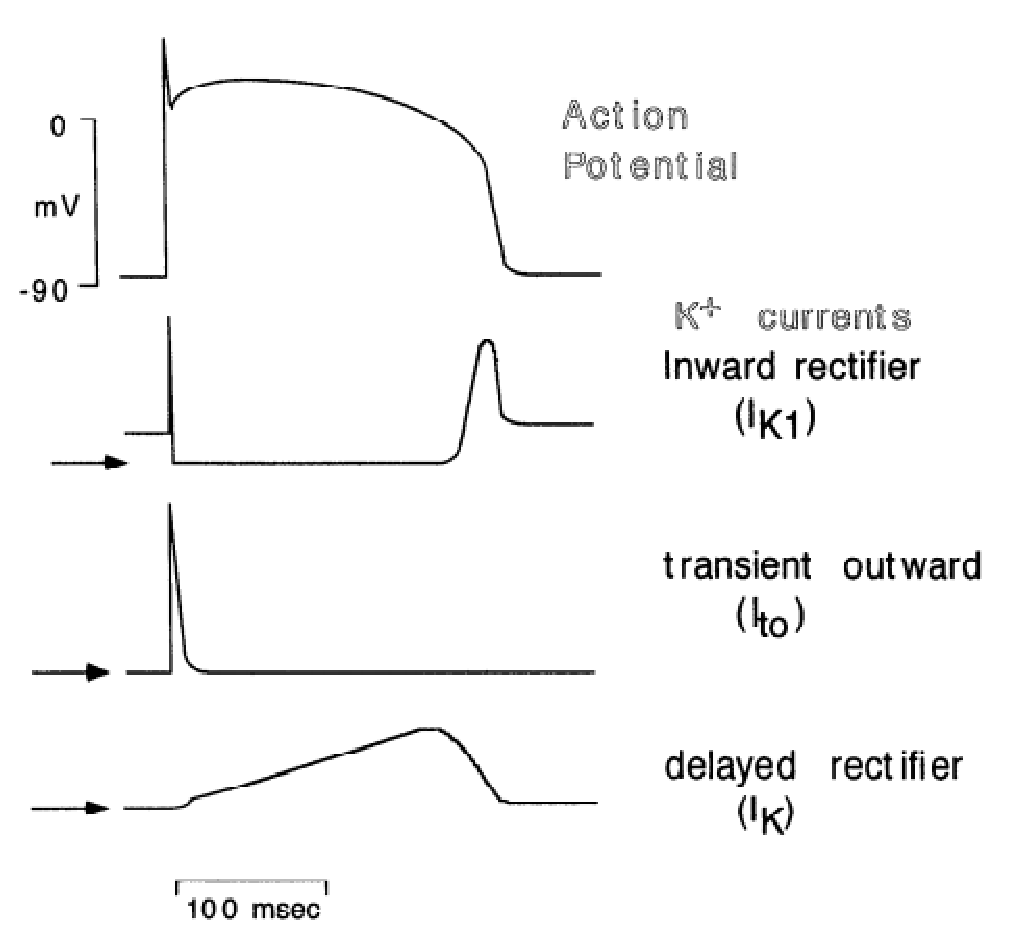
\includegraphics[height=5cm,
    angle=0]{./images/K_current_all.eps}}
  \caption{3 major types of $\K$ currents \citep{sanguinetti1997}}
\label{fig:Kcurrent_all}
\end{figure}

All types of potassium channels in a cardiac cell are shown in
Fig.\ref{fig:K_channel_all}.

\section{Summary}
\label{sec:summary-3}


The concentration of \ce{K+} ions are $10^{16}$ times more
concentrated than internal \ce{Ca^2+} ions. Thus, even if \ce{K+} ions
have a far lower permeability in \ce{Ca} channels than \ce{Ca^2+}
ions, they could still carry more outward current.  


Delayed rectifier $\Kv$ activates during the repolarization, and $\Kir$
involves in maintaining the resting potential (i.e.
$\Kir$ still active at resting potential). The name $\Kv$ only activate slowly
in response to the $V_m$ change during repolarization (repolarization-activated,
not depolarization-activated). [NOTE: {\bf rectification}  refers to the
property of non-linearity in conductance change and voltage \citep{hille1992mb}.
The polarity is called inward if the (positive) ions get into the cell through
channels more easily than they get out; and outward rectification if vice
versa.]

\begin{framed}

There can be different degree of rectification for inward or outward
rectification. Strong inward rectifier Potassium current K$_\ir$ is essential
for the stable resting membrane potential, and long plateau of AP in cardiac
myocytes. At $V_m$ to -40mV, there is very little K$_\ir$ flows outwardly to
avoid the short-circuit in the AP (thus minimizing ATP consumption for pumping
out Sodium and Calcium ions)\citep{tanaka1999}.

\end{framed}

In pancreatic beta cells, to avoid $\K$ leak due to hypoxic damage, a thid
family of $\K$ channel activate, which is ATP-sensitive $\K$ channel ($K_\ATP$).
We only add this to the model when ATP is added as a separate variable.

Like $\Na$ channel, transmembrane S4 segment is the $V_m$ sensor. S2 and S3 are
served to protect S4 from irrelevant charges of the lipid bilayer.

The time-independent $I_{K1}$ is improtant during fast phase-3 repolarization.
The time-dependent $I_\k$, $I_\to$ and possibly $I_\Kp$ are important at
late phase-2 (plateau) repolarization and in determining the shape and duration
of APD. NOTE: $I_\k$ is broken down into $I_\Kf$ and $I_\Ks$. 

In guinea-pig ventricular cells, $I_\k$, but not $I_\to$ is responsible for
plateau repolarization. 


\section{Mink-related peptide 2 (MiRP2) associated with Kv3.4}
\label{sec:Kv3.4-MiRP2}
\label{sec:MiRP2-Kv3.4}


MinK-related peptide 2 (MiRP2) assembles with the Shaw family isolate Kv3.4 to
form subthreshold K+ channels in skeletal muscle that set the resting membrane
potential and are associated in mutant form with inherited periodic paralysis.

% %% Local Variables:
% %% mode: latex %% TeX-master: "thermo-stat" %% End:

